% ----- document class and encoding -----%
\documentclass[12pt]{article}

\usepackage{newtxtext,newtxmath}

% ------ formatting ------%
\usepackage{graphicx}
\setkeys{Gin}{draft=false}

% Use US letter sized paper with 1 inch margins
\usepackage[letterpaper,margin=1in]{geometry}

% Double line spacing, including in captions
\linespread{1.5} % For some reason double spacing is 1.5, not 2.0!

% One space after each sentence
\frenchspacing

% Abstract formatting and spacing - no heading
\renewenvironment{abstract}
	{\quotation}
	{\endquotation}

% No date in the title section
\date{}

% Reference section heading
\renewcommand\refname{References and Notes}

% Figure and Table labels in bold
\makeatletter
\renewcommand{\fnum@figure}{\textbf{Figure \thefigure}}
\renewcommand{\fnum@table}{\textbf{Table \thetable}}
\makeatother

% Call the accompanying scicite.sty package.
% This formats citation numbers in Science style.
\usepackage{scicite}

% Provides the \url command, and fixes a crash if URLs or DOIs contain underscores
\usepackage{url}
\PassOptionsToPackage{hyphens}{url} % URL linebreaks

%%%%%%%%%%%% CUSTOM COMMANDS AND PACKAGES %%%%%%%%%%%%

% Authors can define simple custom commands e.g. as shortcuts to save on typing
% Use \newcommand (not \def) to avoid overwriting existing commands.
% Keep them as simple as possible and note the warning in the text below.
% Example:
\newcommand{\pcc}{\,cm$^{-3}$}	% per cm-cubed

%----- simon's modifications -----%
\clubpenalty = 10000
\widowpenalty = 10000 
\displaywidowpenalty = 10000

% Please DO NOT import additional external packages or .sty files.
% Those are unlikely to work with our conversion software and will cause problems later.
% Don't add any more \usepackage{} commands.
\usepackage{subcaption}
\usepackage{multicol}
\usepackage{multirow}
\usepackage{wrapfig}
\usepackage{tabularray}
\usepackage{booktabs}
\UseTblrLibrary{booktabs}
\usepackage{ragged2e}
\usepackage{float}
\usepackage{dcolumn}
\usepackage{rotating}
\usepackage[title,titletoc]{appendix}
\usepackage[colorlinks=false]{hyperref}
\PassOptionsToPackage{hyphens}{url} % URL linebreaks
\usepackage{pdflscape}
\usepackage{tabularx}
\usepackage[table]{xcolor}
\usepackage[export]{adjustbox}
\usepackage[normalem]{ulem}
\usepackage{setspace}

\urlstyle{rm}             % or: \urlstyle{same}
\renewcommand\UrlFont{\rmfamily}
\hypersetup{
    colorlinks=true,
    linkcolor=black,
    urlcolor=black,
    citecolor=black,
    pdfborder={0 0 0}     % remove link boxes
}

\usepackage{array}
\newcolumntype{L}{>{\RaggedRight\arraybackslash}X}
\newcolumntype{C}[1]{>{\centering\let\newline\\\arraybackslash\hspace{0pt}}m{- 1}}
\newcolumntype{R}[1]{>{\raggedleft\let\newline\\\arraybackslash\hspace{0pt}}m{- 1}}
\newcolumntype{T}{>{\raggedright\arraybackslash}m{8cm}}
\newcommand\LL[1]{\multicolumn{1}{c}{- 1}}
\newcommand\RR[1]{\multicolumn{1}{c|}{- 1}}
\newcommand\LR[1]{\multicolumn{1}{|c|}{- 1}}


%%%%%%%%%%%%%%%% TITLE AND AUTHORS %%%%%%%%%%%%%%%%

% Title of the paper.
% Keep it short and understandable by any reader of Science.
% Avoid acronyms or jargon. Use sentence case.
\def\scititle{
	Myside Bias Undermines Online Content Moderation
}
% Store the title in a variable for reuse in the supplement (otherwise \maketitle deletes it)
\title{\bfseries \boldmath \scititle}

% Author and institution list.
% Institution numbers etc. should be hard-coded, do *not* use the \footnote command.
\author{
    Simon~Munzert$^{1\ast}$,
    Julia~Ellingwood$^{2}$,
    Lisa~Oswald$^{3}$,
    Richard~Traunmüller$^{4}$\and
    \small$^{1}$Data Science Lab, Hertie School\and
    \small$^{2}$King's College London\and
    \small$^{3}$Centre for Critical Communication Studies, University of Frankfurt and
    \small$^{4}$University of Mannheim\and
    \small$^\ast$Corresponding author. Email: munzert@hertie-school.org
}
%%%%%%%%%%%%%%%%% END OF PREAMBLE %%%%%%%%%%%%%%%%

%%%%%%%%%%%%%%%% START OF MAIN TEXT %%%%%%%%%%%%%%%
\begin{document} 

% Insert the title and author list
\maketitle

% Abstract, in bold
% There are strict length limits, and not all formats have abstracts.
% Consult the journal instructions to authors for details.
% Do not cite any references in the abstract.

\newpage

\begin{abstract}

\hyphenpenalty=5000\emergencystretch=1em

\textbf{Online content moderation shapes what billions of people can say and see, yet the human judgments that train and evaluate moderation systems are themselves contested. Drawing on a pre-registered cross-national conjoint experiment with 19{,}172 respondents across 11 countries, we analyze over 150{,}000 moderation judgments of toxic social media posts. We find robust evidence of \emph{myside bias}: people are substantially more likely to classify speech as hateful and to support sanctions against it when the attacked target shares their position on the contested issue at hand. This pattern holds across countries, political camps, topics, and speech types, and is larger in magnitude than effects of gender, ideology, or ethnic identity. These results reveal a fundamental challenge for content moderation: systematic disagreement in moderation judgments is tied also to the \emph{content} of beliefs, not only to fixed annotator characteristics. This means that standard bias-correction approaches---which adjust for stable demographic or partisan attributes---cannot resolve the underlying disagreement, posing a structural challenge for the governance of automated enforcement in polarized environments.}

\end{abstract}

\noindent
Content moderation shapes what billions of people can say and see online, yet the judgments underpinning it are deeply contested~\cite{trujilloDSATransparencyDatabase2025}. 
Automated moderation systems face well-documented technical limits: harmful content slips through while benign speech is wrongly removed~\cite{hartmannLostModerationHow2025,faschingModelDependentModerationInconsistencies2025}. But these inconsistencies are not merely engineering failures. At their root, they reflect a more fundamental problem: judgments about what counts as hateful or legitimate speech are inherently subjective~\cite{plankProblemHumanLabel2022}, shaped by cultural norms~\cite{jiangUnderstandingInternationalPerceptions2021}, moral values~\cite{davaniDisentanglingPerceptionsOffensiveness2024}, racial attitudes~\cite{sapAnnotatorsAttitudesHow2022,waltersMoralDisengagementContent2025}, and group identity~\cite{dasInvestigatingAnnotatorBias2024,giorgiHumanLLMBiases2025,garg_handling_2023,wilhelmGenderedMoralityBacklash2019}. Modern AI systems inherit these tensions because they learn from human annotations---but when human annotators systematically disagree, there is no stable ground truth to learn from~\cite{plankProblemHumanLabel2022}.

% recent evidence
Research on moderation judgments has identified two main sources of systematic disagreement. The first is \emph{identity bias}: variation in how speech is classified depending on the demographic characteristics of the annotator or the target---such as gender, race, or religion~\cite{dasInvestigatingAnnotatorBias2024,giorgiHumanLLMBiases2025,sapAnnotatorsAttitudesHow2022,wilhelmGenderedMoralityBacklash2019}. The second is \emph{partisan bias}: the tendency to judge speech more harshly when it attacks one's own political camp~\cite{appelPartisanConflictContent2023,Lindner2009,munzertCitizenPreferencesOnline2025}. Evidence for both patterns exists in annotation studies and in survey experiments on public moderation preferences~\cite{pradelGenderDifferencesDemanding2024}, though findings on partisan bias in particular remain mixed: Munzert et al.~\cite{munzertCitizenPreferencesOnline2025} find indications of partisan in-group favoritism, while Pradel et al.~\cite{pradelGenderDifferencesDemanding2024} and Rasmussen et al.~\cite{rasmussenLimitedEffectsTarget2024} report little such evidence. A key limitation of this literature, however, is that partisan and identity-based accounts treat disagreement as a function of \emph{who} the annotator is---their party, gender, or ethnicity. This leaves open the possibility that a more dynamic, content-contingent form of bias is at work: one rooted not in stable personal characteristics but in what people \emph{believe}.

% what we do
Here, we suggest and test for another important source for disagreement on what offensive and hateful speech is and what should be done about it. In addition to identity bias, we show that perceptions and preferences are also the product of a self-serving cognitive \emph{myside bias}: people’s willingness to see speech as hateful—and to support sanctions against it—depends crucially on whether they agree or disagree with the political stance of the position being attacked~\cite{stanovichBiasThatDivides2021}. This bias not only undermines the reliability of training data, but also reinforces pressing normative questions: whose voices should content moderation algorithms amplify, and whose values should they represent~\cite{gordonJuryLearningIntegrating2022,webbwilliamsWhenConservativesSee2023}?

% our argument
As a specific form of motivated reasoning, the relevance of myside bias extends well beyond the phenomenon of ``mere'' partisan bias. Unlike more stable identity-based biases, which can often be documented and statistically adjusted for, myside bias is more fundamental: it reaches beyond partisans, can operate in non-political domains (e.g., reasoning about health choices, religion, or personal values), and is uncorrelated with intelligence or cognitive ability~\cite{stanovichNaturalMysideBias2007,stanovichFailureCognitiveAbility2008}. What further sets myside bias apart from identity- or partisan-based biases is that it is not a personal characteristic of individuals who hold beliefs, but a feature of the beliefs themselves and their specific content~\cite{stanovichBiasThatDivides2021}. 
It emerges dynamically, issue by issue, as individuals selectively interpret speech in light of their own convictions (see~\cite{roozenbeekSusceptibilityMisinformationConsistent2022} for parallels in the domain of misinformation). This makes it particularly difficult to correct for in both annotation and modeling, since no fixed adjustment can account for the shifting contours of political disagreement. 

% our contributions: identify myside bias and collecting lots of data
Our study expands the existing body of evidence in two important ways: First, we study moderation decisions at scale across a large set of topics and speech acts, balancing partisans stances, and measure participants' beliefs on a wide variety of topics, not just ideology. This allows us to disentangle myside from partisan bias. 

% what we do 2: collecting lots of data
Second, we examine preferences across a diverse set of eleven countries spanning both the Global North and South, representing more than a third of the world's population. Much of the existing evidence—often centered on the United States—suggests that conflict over content moderation is primarily driven by partisanship, that is, whether content benefits or harms one’s own party~\cite{appelPartisanConflictContent2023,solomonIllusoryInterpartyDisagreement2024,christopherstaubinMostAmericansFavor2023}. Yet the extreme polarization observed in the U.S. may not generalize to other contexts. Furthermore, judgments on speech might also vary across cultures shaped by distinct historical experiences and moral principles. Comparative evidence is therefore crucial to assess whether such patterns hold globally across different cultural contexts and norms of free expression. This also matters because online speech is moderated in a transnational environment: both exposure to content and the enforcement of moderation policies occur across national boundaries. If perceptions of what counts as harmful or legitimate speech diverge substantially across contexts, the legitimacy and effectiveness of current moderation practices are called into question.

%--- DESIGN ---%
\section*{Design and Data}

To estimate the role of myside bias relative to other sources of disagreement in content moderation, we embedded a conjoint experiment in a cross-sectional online survey fielded in eleven countries: Brazil, Colombia, Germany, India, Indonesia, Nigeria, the Philippines, Poland, Turkey, the United Kingdom, and the United States. Countries were selected to maximize regional diversity and variation in free speech norms~\cite{skaaningWhoCaresFree2021}, spanning democracies and hybrid regimes, the Global North and South, and contexts ranging from high to low political polarization. Full details on participant recruitment, experimental setup, measurement, and statistical analyses are provided in the Materials and Methods section.

\begin{figure}
  \centering
    % Subfigure A
  \begin{subfigure}[t]{1\textwidth}
  \centering
    \caption*{\textbf{A}} 
    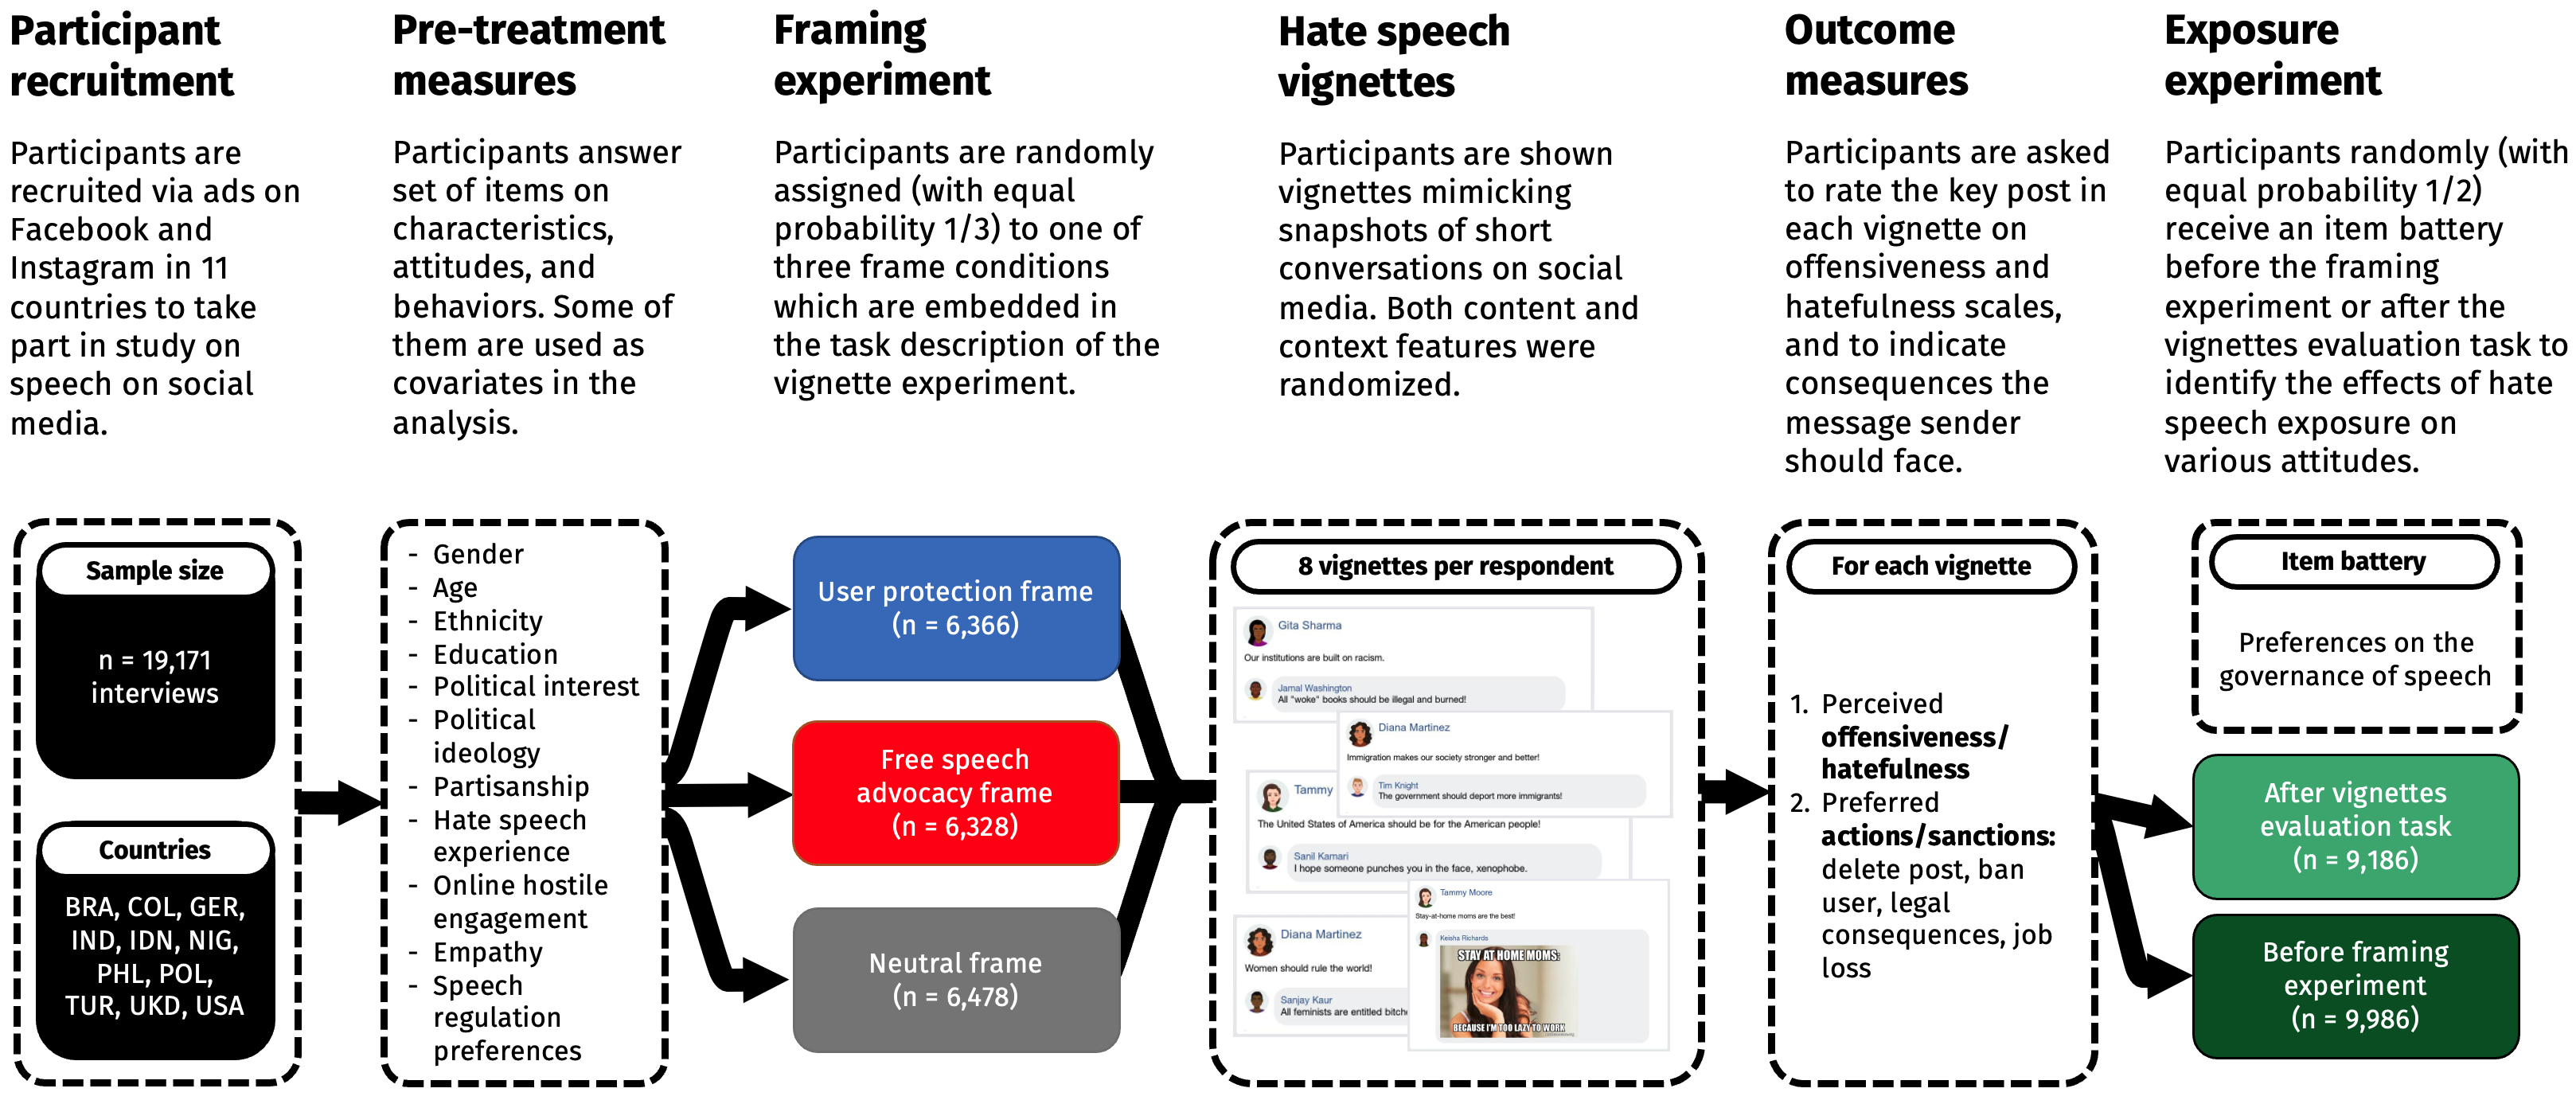
\includegraphics[width=1\linewidth]{figures/design-setup.png}
  \end{subfigure}
  \hfill
  % Subfigure B
  \begin{subfigure}[t]{.49\textwidth}
  \centering
    \caption*{\textbf{B}} 
    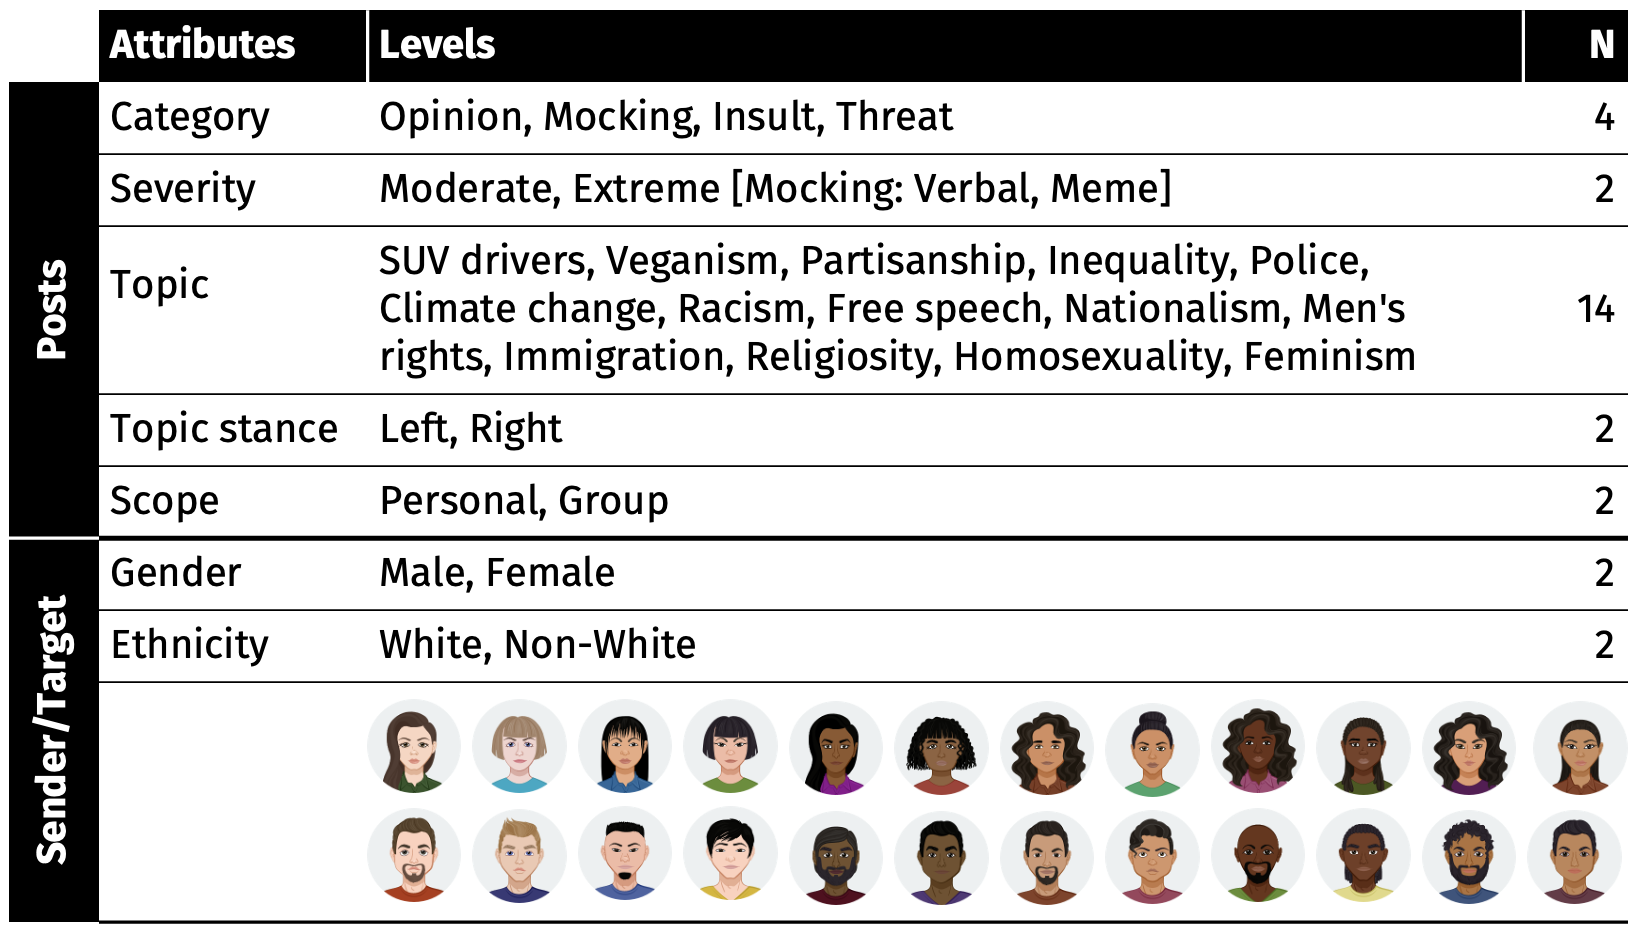
\includegraphics[width=1\linewidth]{figures/vignette-attributes-overview.png}
  \end{subfigure}
  \hfill
  % Subfigure C
  \begin{subfigure}[t]{.49\textwidth}
    \centering
    \caption*{\textbf{C}}
    \includegraphics[width=1\linewidth]{figures/vignette-examples-3.png}
  \end{subfigure}
\caption{\textbf{Study design overview.} \textbf{(A)} Participants from 11 countries were randomly assigned to one of three platform framing conditions before evaluating 8 speech vignettes in a moderation task. Placement of the moderation task within the survey was also randomized between subjects to assess short-term exposure effects. \textbf{(B)} Attributes and levels used to construct synthetic social media conversations, yielding $N_{\text{msg}} = 387$ unique sender messages and $N_{\text{vig}} = 31{,}484$ unique sender--target conversation pairs shown to respondents. \textbf{(C)} Two example conversations on the immigration topic, illustrating a left-leaning and a right-leaning target position and their associated attribute levels.}
\label{fig:design-overview}
\end{figure}

Respondents evaluated short, synthetic social media exchanges in which a sender responded to a target's post. The target's post expressed a clear stance on one of 14 politically contested issues; the sender's message varied in type and severity, from opinion statements and mockery to insults and explicit threats. Both sender and target were assigned fictitious names and cartoon avatars that signaled gender and ethnicity. Vignette attributes---including issue topic, target stance, sender message type and severity, and sender and target identity characteristics---were independently randomized, allowing us to isolate the contribution of each component to moderation judgments. Figure~\ref{fig:design-overview} provides an overview of the design and sample vignettes; a complete listing of all stimulus materials is provided in SI section~\ref{si:posts}.

By embedding realistic speech examples in a conversational social media format, the design offers greater ecological validity than abstract free-expression survey items while retaining full experimental control over the features we manipulate. In natural online environments, the identity of the speaker, the severity of the message, and the political content of the target's post are confounded; our design varies each independently, enabling clean identification of myside and identity bias effects.

Relative to prior vignette-based work on moderation preferences~\cite{munzertCitizenPreferencesOnline2025}, the present study extends the stimulus set in three ways. First, we include meme-based speech---visually enriched content that combines image and text---which poses distinctive challenges for automated moderation due to its multimodal nature and dependence on cultural context~\cite{kielaHatefulMemesChallenge2020}. Second, we cover 14 topics and ensure that each topic includes both left- and right-leaning target positions, so that any estimated myside effect cannot be an artifact of ideological imbalance in the vignette pool. Third, we field the design across eleven countries, allowing us to assess whether the pattern is global or context-specific.

For each of the eight vignettes each respondent evaluated, we measured six outcomes spanning perception and preferred action. For perception, respondents classified the sender's message as hate speech, offensive but not hate speech, or neither offensive nor hateful; we treat this as two binary dependent variables (hate speech vs. not; offensive-or-worse vs. neither). For preferred action, respondents indicated in binary format whether the post should be removed from the platform, whether the sender should be banned, whether the sender should face legal consequences, and whether the sender should face consequences from their employer. This yields 153,376 judgments across the pooled sample.

To measure myside bias, we surveyed respondents' agreement with the same issue statements that later appear as target positions in the vignettes, prior to the experiment. For each respondent-vignette pair, we derive a binary indicator of issue-stance alignment: whether the respondent agrees with the position the target is defending. Myside bias is then estimated as the effect of that alignment on moderation judgments (pre-registered hypothesis 1; SI section~\ref{si:pap}). Because alignment is measured at the issue level rather than the ideological level, this approach separates myside bias from general left-right partisanship: respondents who lean left may align with a target on climate policy but not on immigration, and the design captures both.

To estimate identity bias separately from myside bias, we also measure gender and ethnicity overlap between respondents and vignette characters. Early in the survey, respondents selected from the same set of cartoon avatars used in the vignettes the one they felt most closely resembled them, providing a direct measure of perceived in-group membership rooted in social identity~\cite{grantValueConflictGroup2003}. We use gender and ethnicity match between respondent and target (or sender) as the basis for testing in-group favoritism in moderation judgments (pre-registered hypotheses 2 and 3; SI section~\ref{si:pap}), focusing on these two characteristics because prior annotation research has shown them to systematically affect hate speech classifications~\cite{dasInvestigatingAnnotatorBias2024,giorgiHumanLLMBiases2025}. We note that stylized avatars provide a conservative and relatively weak operationalization of identity cues compared to photographs or named profiles; the identity bias estimates reported below should be interpreted accordingly.


\begin{figure}
  \centering
  % Subfigure A
  \begin{subfigure}[t]{1\textwidth}
  \centering
    \caption*{\textbf{A}} 
    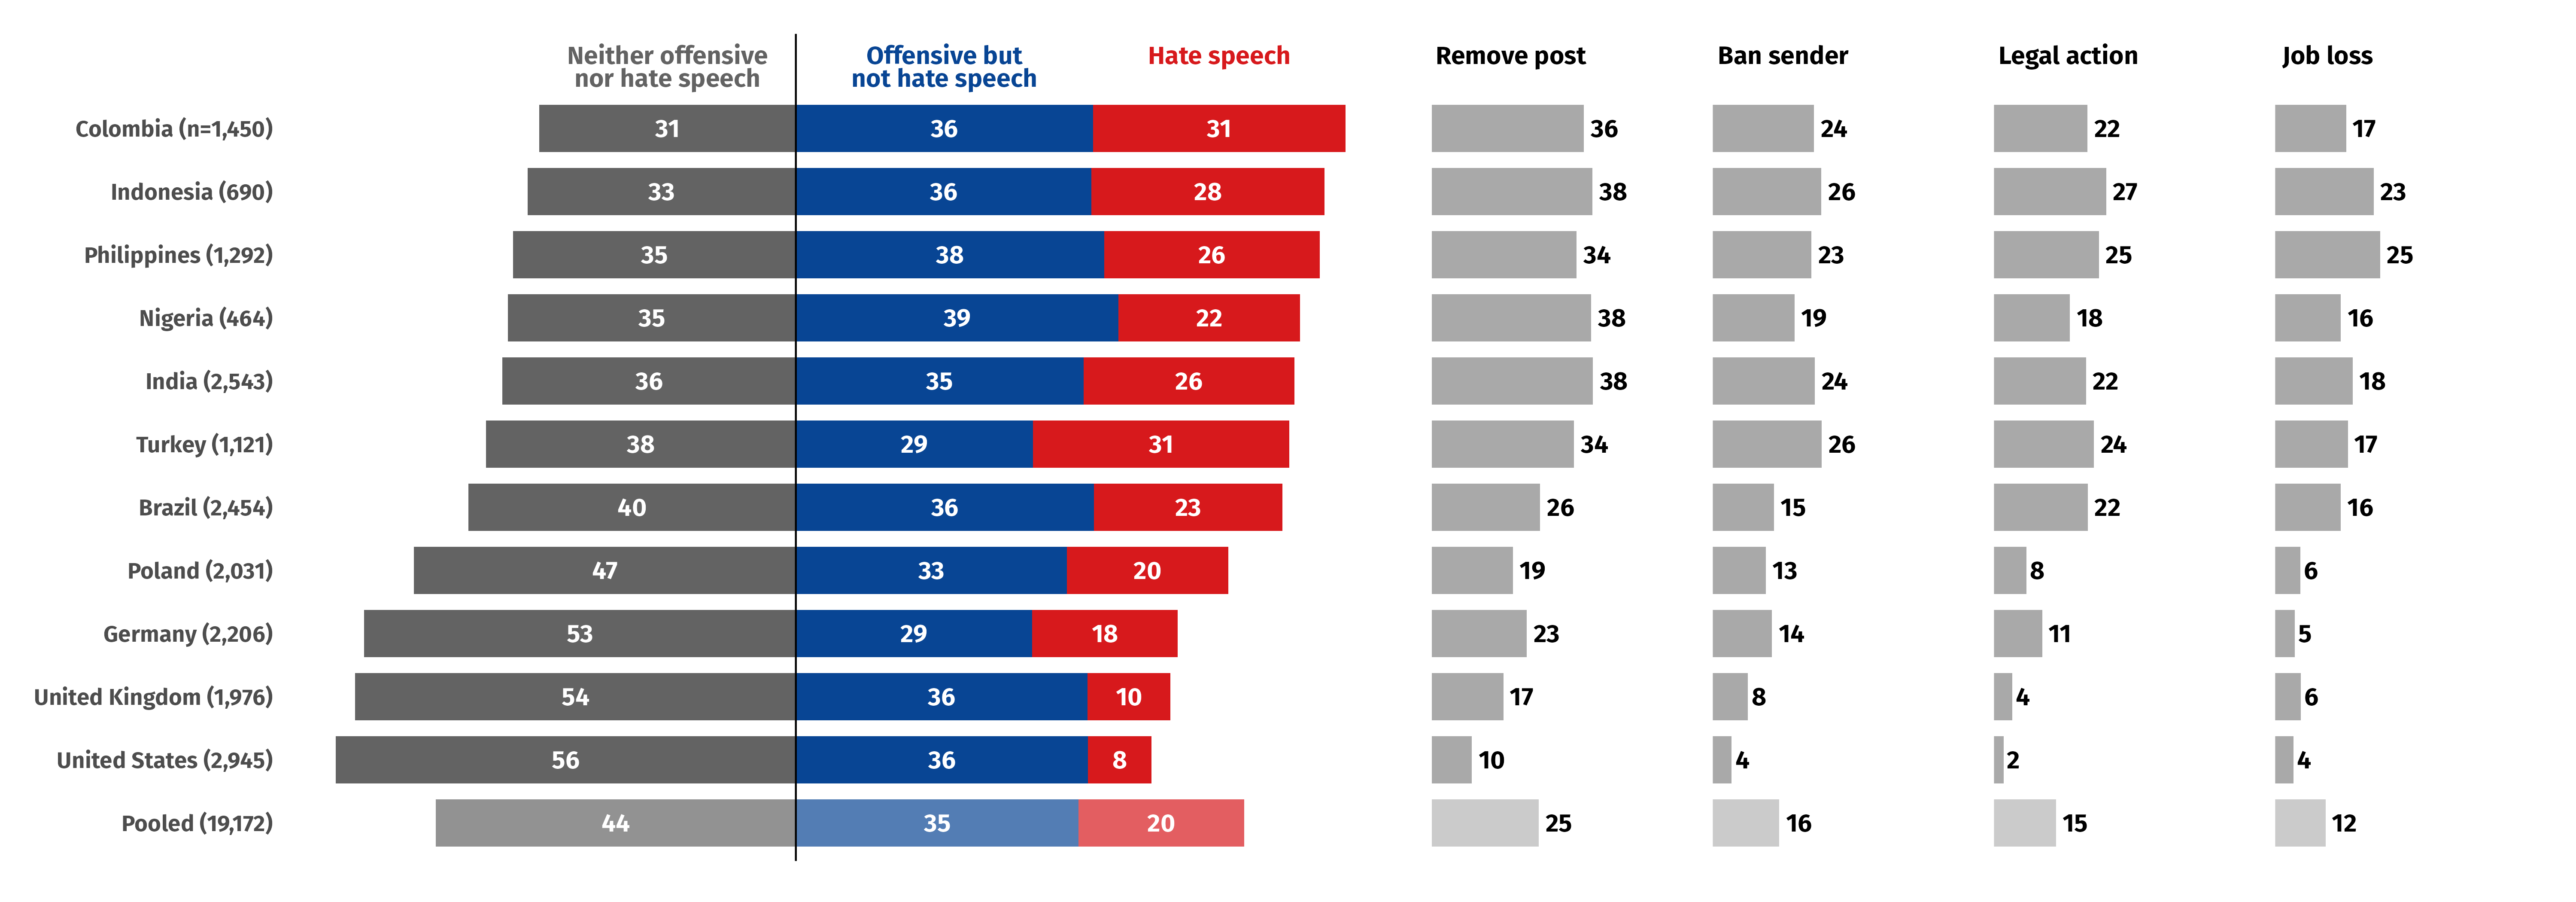
\includegraphics[width=1\linewidth]{figures/barplot-perceptions-actions-by-country.png}
  \end{subfigure}
  \hfill
  % Subfigure B
  \begin{subfigure}[t]{1\textwidth}
    \centering
    \caption*{\textbf{B}}
    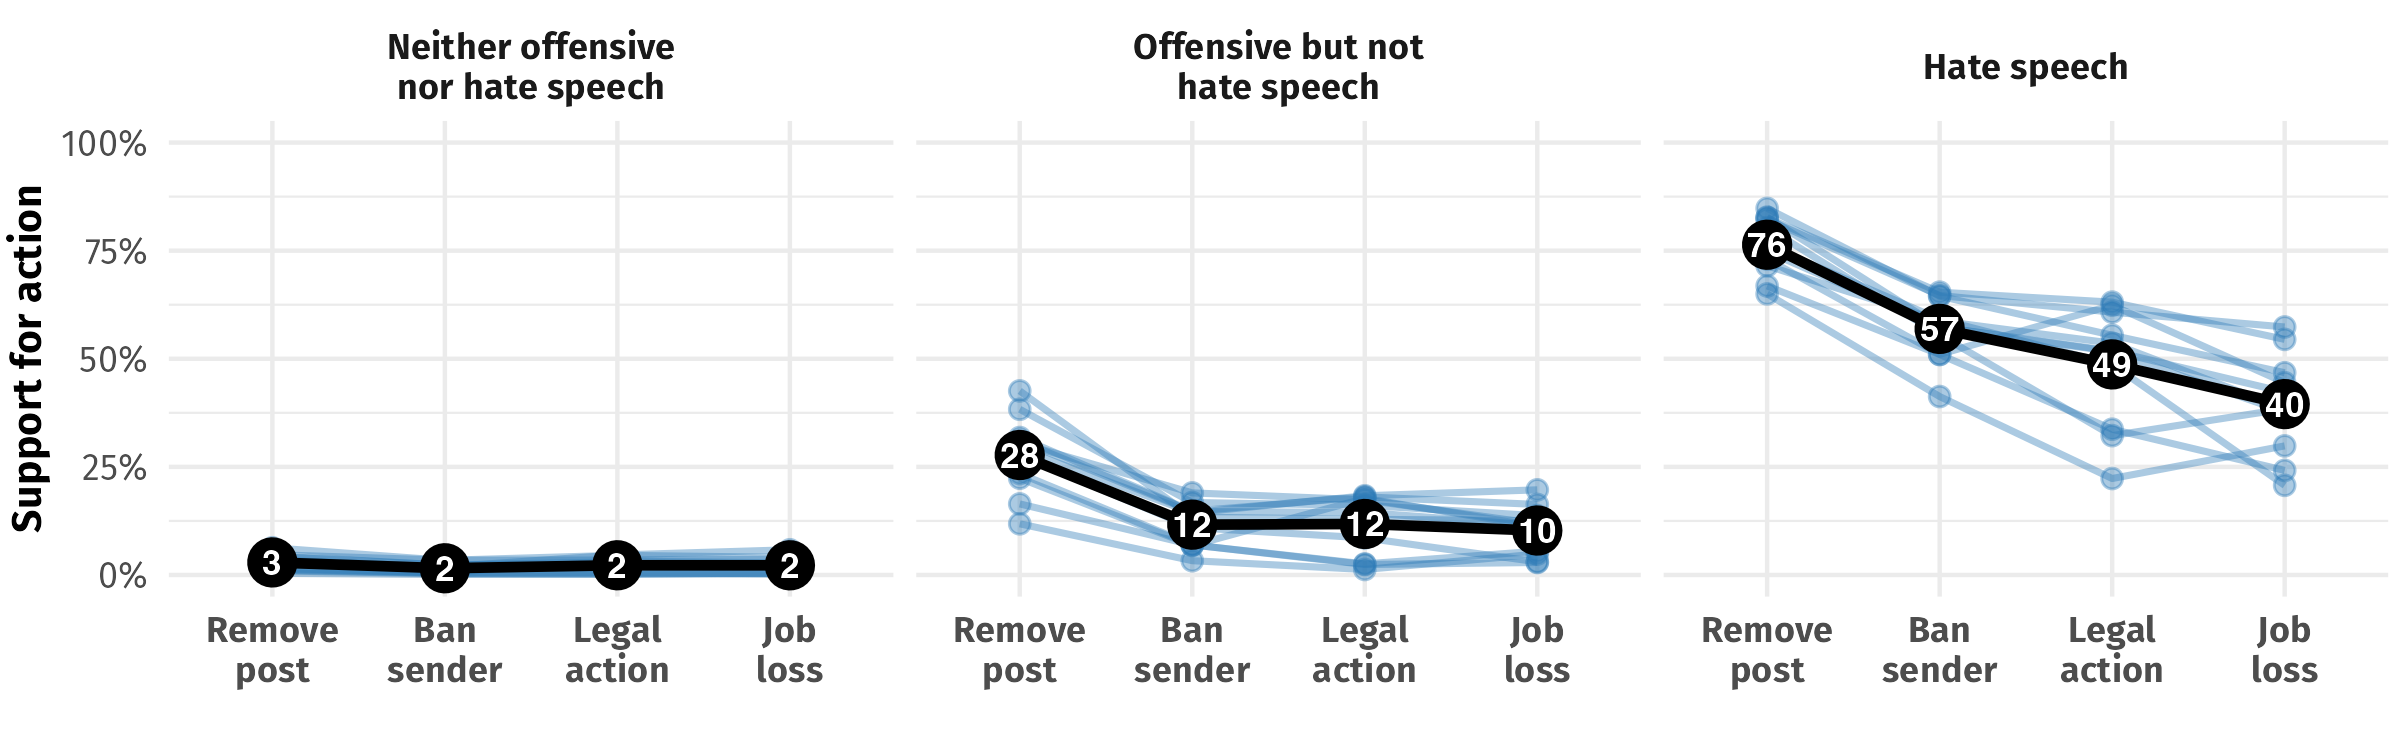
\includegraphics[width=1\linewidth]{figures/profileplot-actions-by-perceptions.png}
  \end{subfigure}
\caption{\textbf{Speech perceptions and sanctioning preferences across countries.} \textbf{(A)} Proportion of vignettes classified as hate speech, offensive speech, or neither, and proportion of respondents supporting each sanction type, by country. Country-level differences reflect both genuine cross-national variation in norms and potential differences in sample composition; see main text. \textbf{(B)} Sanctioning preferences conditional on speech perception. Lines show the share of respondents supporting each action for content classified as hate speech, offensive but not hate speech, or neither offensive nor hateful; black lines represent pooled estimates and blue lines represent country-specific estimates. Based on 153,376 judgments by 19,172 participants.}
\label{fig:profileplot-actions-by-perceptions}
\end{figure}

%--- RESULTS ---%
\section*{Results}

Our results reveal three main patterns. First, there is no universal standard for what qualifies as offensive or hateful speech: perceptions and sanctioning preferences vary substantially across countries and respondents, though a consistent hierarchy emerges in which perceived hate speech commands much broader support for removal (roughly three out of four or 76\% of all judged posts) and other sanctions than speech perceived as merely offensive (less than one in three posts or 28\%; Fig.~\ref{fig:profileplot-actions-by-perceptions}). Second, respondent characteristics shape moderation preferences to a modest degree---women and ideologically left-leaning respondents are generally more supportive of intervention (Fig.~\ref{fig:table-respmodels-pooled}). Third, and most consequentially, we find robust evidence of myside bias across all six outcomes, all eleven countries, both political camps, and all 14 topics: respondents who share a target's issue position are substantially more likely to classify attacks on that target as hateful and to support sanctions against the sender (Figs.~\ref{fig:effects-h1-3-coefplot-flipped} and~\ref{fig:effects-h1-coefplot-heterogeneity}). In contrast, we find no evidence of identity-based in-group favoritism as a function of gender or ethnicity overlap under the avatar-based operationalization used here. We elaborate each finding in turn.

Fig.~\ref{fig:profileplot-actions-by-perceptions} presents an overview of perceptions and sanctioning preferences across the pooled sample and by country. Panel A shows substantial cross-national variation in baseline classification rates: for instance, 31\% of cases in the Colombian sample were classified as hate speech compared to 8\% in the United States. These country-level differences reflect both genuine cross-national variation in norms and thresholds and potential differences in sample composition arising from platform-based recruitment; they should be interpreted as descriptive patterns rather than precise population estimates. Across all countries, pooled classification rates were 20\% hate speech and 35\% offensive speech. A consistent pattern across countries is that platform-based sanctions---post removal and user bans---command broader support than offline consequences such as legal action or job loss.

Panel B shows that perceptions of speech are closely tied to sanctioning preferences. Content classified as neither offensive nor hateful is almost universally left unsanctioned. Offensive-but-not-hateful speech draws limited intervention support, with some backing for removal but little for harsher measures. When content is perceived as hate speech, support for removal and sender-directed sanctions rises markedly, with considerable backing even for offline consequences such as legal proceedings or job loss. It is worth noting that our stimulus set deliberately skews toward contentious content---ranging from provocative policy opinions and mockery to explicit threats---rather than innocuous speech. Even so, many respondents decline to endorse sanctions against content they classify as hateful, underscoring a broadly tolerant baseline that makes the myside bias effects we report below all the more notable.

\paragraph{Content-level drivers of moderation preferences.}

The type and severity of the sender's message are the strongest content-level predictors of moderation judgments, replicating the hierarchy documented in prior vignette research~\cite{munzertCitizenPreferencesOnline2025,pradelToxicSpeechLimited2024,rasmussenLimitedEffectsTarget2024} and extending it to a broader range of speech types and countries (Figs.~\ref{fig:table-acme-pooled} and~\ref{fig:table-mm-pooled}). Threatening content elicits the harshest reactions; mocking, meme-based, and opinion speech is judged far less severely; insulting content falls in between. Topic also matters: speech targeting core identity issues such as gender, sexuality, or religion is sanctioned more heavily than speech on policy topics. By contrast, the demographic characteristics of the sender and target---their gender and apparent ethnicity---have no sizable effect on perceptions or sanctioning preferences. This absence of identity-feature effects on the content side is consistent across all six outcomes and all eleven country samples (Figs.~\ref{fig:table-acme-vig_perc_offensive2}--\ref{fig:table-acme-vig_perc_job}).

\paragraph{Respondent-level drivers of moderation preferences.}

Our rich respondent data allow us to examine how perceptions of the toxicity of online speech correlate with sociodemographic factors, political attitudes, relevant psychological constructs, and reported online behavior (see Fig.~\ref{fig:table-respmodels-pooled}). We highlight here only those findings that prove robust across most contexts (see also the country-level models in Fig.~\ref{fig:table-respmodels-vig_perc_offensive2} to~\ref{fig:table-respmodels-vig_job}). Women are more likely than men to perceive posts as offensive ($+5.3$ pp; $p < 0.01$) and to support removal ($+7.1$ pp; $p < 0.01$), a pattern consistent with prior work on gendered differences in toxicity judgments~\cite{munzertCitizenPreferencesOnline2025,sapAnnotatorsAttitudesHow2022}; effects of age and education are weaker and less consistent~\cite{orlikowskiEcologicalFallacyAnnotation2023}. Respondent ethnicity shows no consistent association with moderation preferences, adding to mixed prior evidence~\cite{rottgerTwoContrastingData2022,jiangUnderstandingInternationalPerceptions2021} and providing a further indication that identity-based effects in this domain are modest. Politically right-leaning respondents support removal less often than left-leaning respondents ($-4.0$ pp; $p < 0.01$)~\cite{sapAnnotatorsAttitudesHow2022,webbwilliamsWhenConservativesSee2023}. Among behavioral predictors, prior targets of toxic speech are more sensitive to hateful content, while respondents who report hostile online engagement are less so, consistent with exposure-based desensitization accounts~\cite{meersonTooMuchWhat2025}.

\begin{figure}
  \centering
    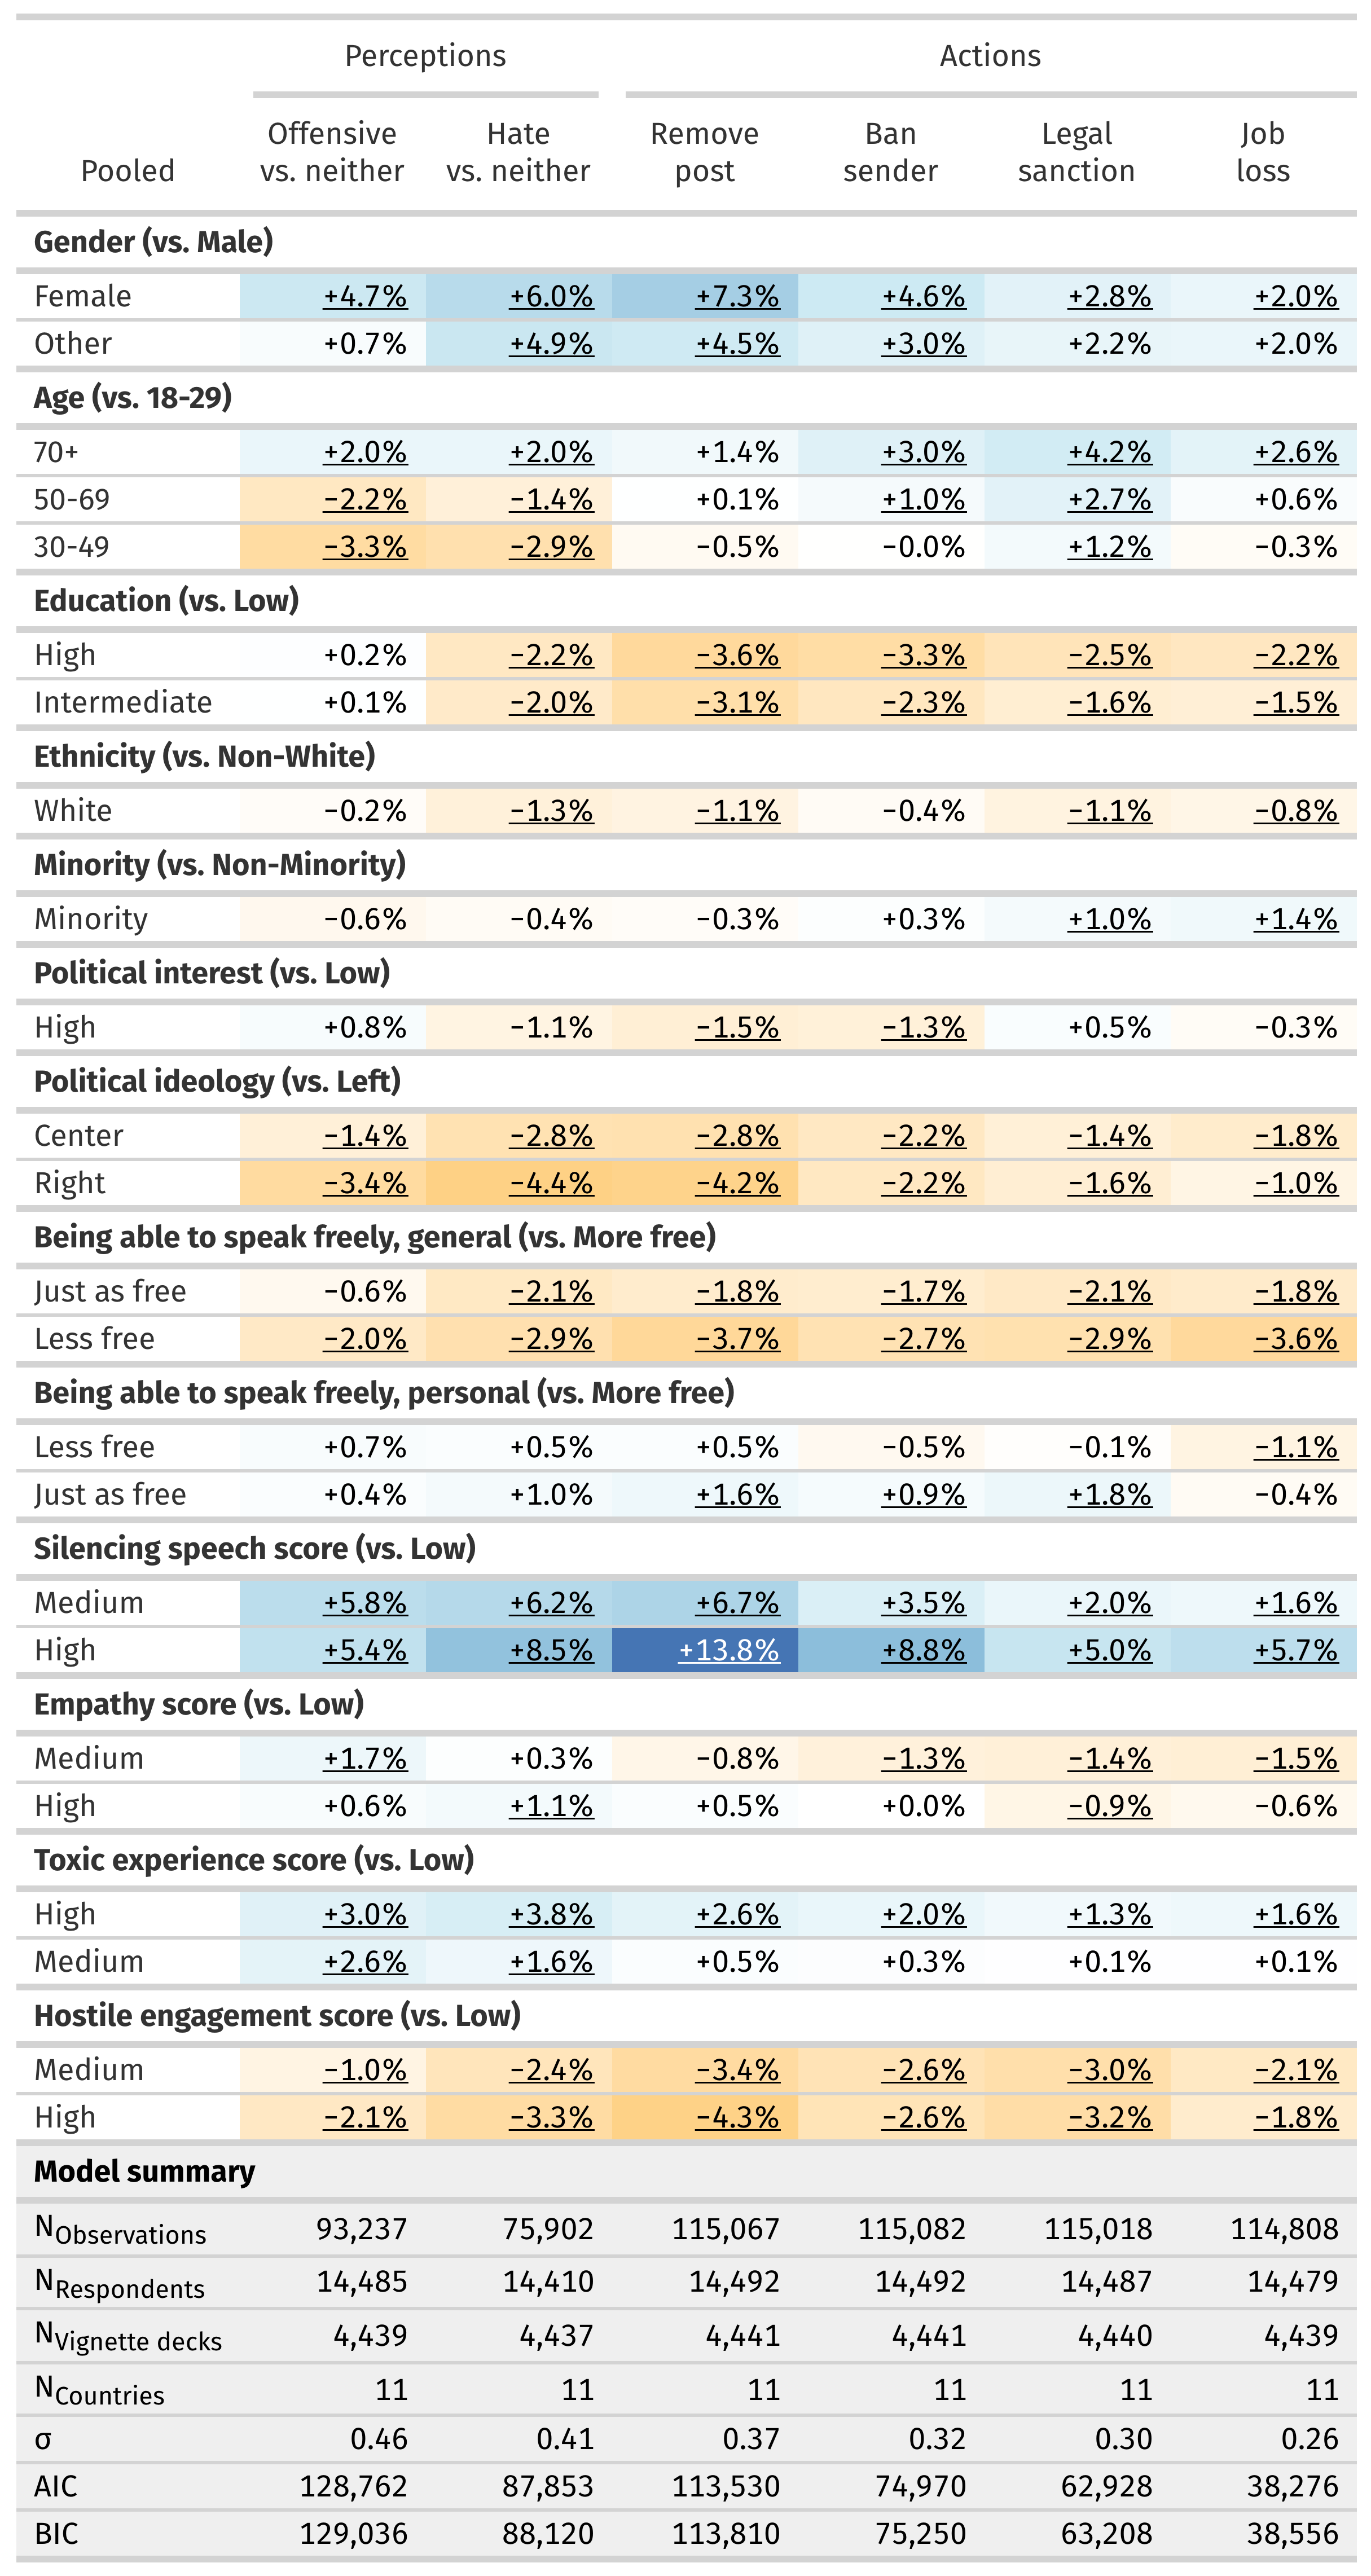
\includegraphics[width=.7\linewidth]{figures/table-respmodels-pooled.png}
\caption{\textbf{Respondent characteristics as predictors of moderation judgments.} Estimated from hierarchical linear probability models with respondent, vignette deck, and country random effects. All outcomes are binary. Estimates represent percentage-point differences in outcome probabilities relative to the reference category; underlined estimates are statistically significant at $p < 0.05$. Color shading indicates effect size. Country-specific results are shown in SI Figs.~\ref{fig:table-respmodels-vig_perc_offensive2}--\ref{fig:table-respmodels-vig_job}.}
\label{fig:table-respmodels-pooled}
\end{figure}

\paragraph{Strong evidence for my-side bias, no evidence for identity bias.} 

Issue-stance alignment between respondent and target is a strong and consistent predictor of moderation judgments across all six outcomes (Fig.~\ref{fig:effects-h1-3-coefplot-flipped}, column 1). Respondents who agree with the attacked target's position are more likely to classify the sender's message as offensive ($+7.3$ pp), as hate speech ($+6.0$ pp), and to support post removal ($+6.4$ pp), user bans ($+5.2$ pp), legal consequences ($+3.9$ pp), and job loss ($+3.9$ pp; all $p < 0.01$). These effects are almost uniformly positive and statistically significant across country samples. To convey practical magnitude: the predicted probability of supporting removal is $31.7$ pp when the respondent agrees with the target's issue position, compared to $25.4$ pp when they disagree---a difference larger than most respondent-level main effects including gender and ideology.

\begin{figure}
  \centering
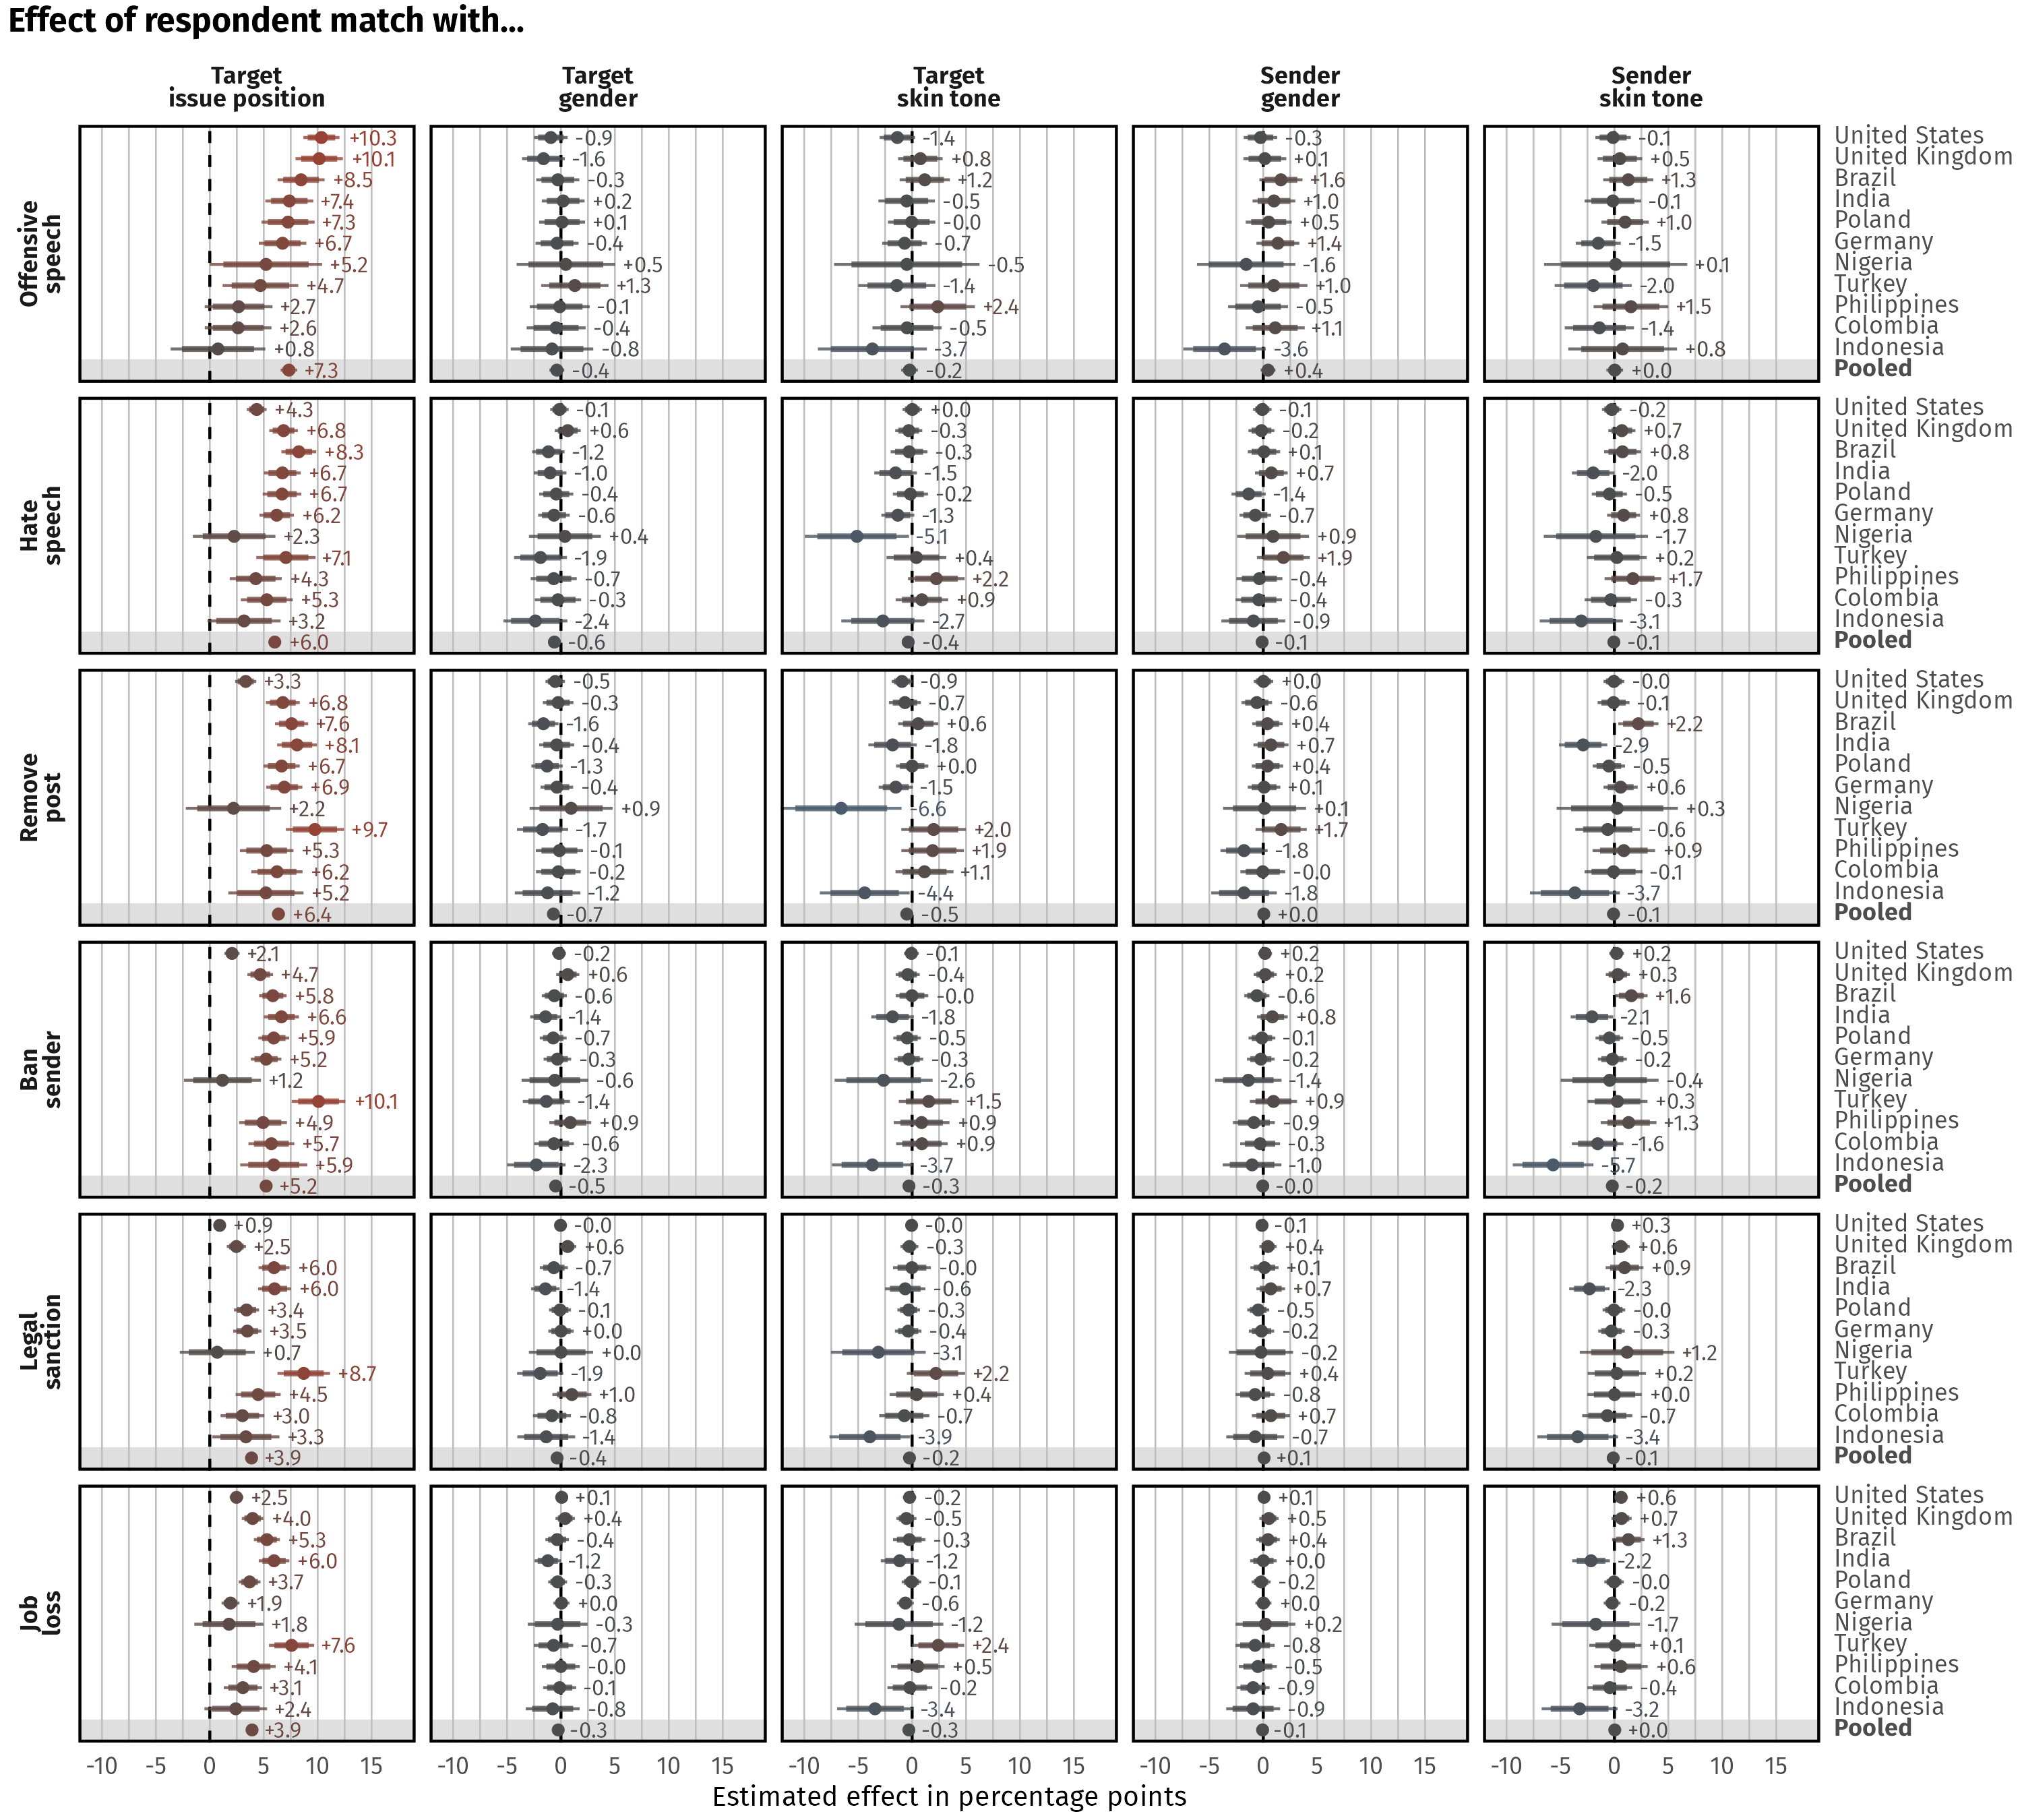
\includegraphics[width=1\linewidth]{figures/effects-h1-3-coefplot-flipped.png}
\caption{\textbf{Myside bias and identity bias in moderation judgments.} Estimates from pooled hierarchical linear probability models with respondent, vignette deck, and country random effects. Each point represents the percentage-point difference in outcome probability when respondent and target share the relevant characteristic (issue stance, gender, or skin tone) compared to when they do not. Column 1 shows myside bias (issue-stance alignment between respondent and target); columns 2--3 show gender and skin-tone alignment with the target; columns 4--5 show gender and skin-tone alignment with the sender. All outcomes are binary. Horizontal lines show 95\% and 99\% confidence intervals.}
\label{fig:effects-h1-3-coefplot-flipped}
\end{figure}

By contrast, gender and skin-tone alignment with the target or sender show no consistent association with moderation judgments under the avatar-based operationalization used here (Fig.~\ref{fig:effects-h1-3-coefplot-flipped}, columns 2--5). Most pooled estimates are close to zero and precisely estimated.

Heterogeneity analyses show that myside bias is robust across contexts but varies in intensity (Fig.~\ref{fig:effects-h1-coefplot-heterogeneity}). The bias in perceiving messages as offensive is attenuated when speech is more extreme---insults and threats trigger strong reactions regardless of stance alignment---but hate speech classifications and sanctioning preferences remain strongly shaped by alignment even as message severity increases. Among topics, the largest myside effects are observed for homosexuality, where stance alignment substantially amplifies differences across all outcome measures, likely reflecting the high attitudinal polarization on this issue across our country samples.

Among respondent characteristics, gender shows no consistent association with the strength of myside bias. Political orientation, however, reveals a pattern: left-leaning respondents show moderately stronger myside bias than centrist or right-leaning respondents, particularly for removal preferences ($+8.6$ pp vs. $+5.0$ pp; difference significant at $p < 0.01$). Also, respondents who strongly endorse the idea that offensive voices should be silenced are not only more supportive of content moderation overall, but also apply myside bias more forcefully than others, indicating stronger double standards.

Taken together, the results establish myside bias as a pervasive feature of content moderation judgments. No subgroup or content type is immune: across all 14 topics, all speech types, all 11 countries, and both political camps, alignment with the attacked target reliably increases perceived offensiveness and support for sanctions. The magnitude of the effect varies---attenuated when speech is extreme, amplified by attitudinal predispositions toward silencing---but the direction is uniform. Crucially, moderation preferences are shaped more by respondents' agreement with the political content of the post than by the demographic identity of those involved. Because myside bias shifts dynamically across issues rather than tracking stable annotator characteristics, it cannot easily be addressed by demographic debiasing or partisan-balance adjustments.

\begin{figure}
  \centering
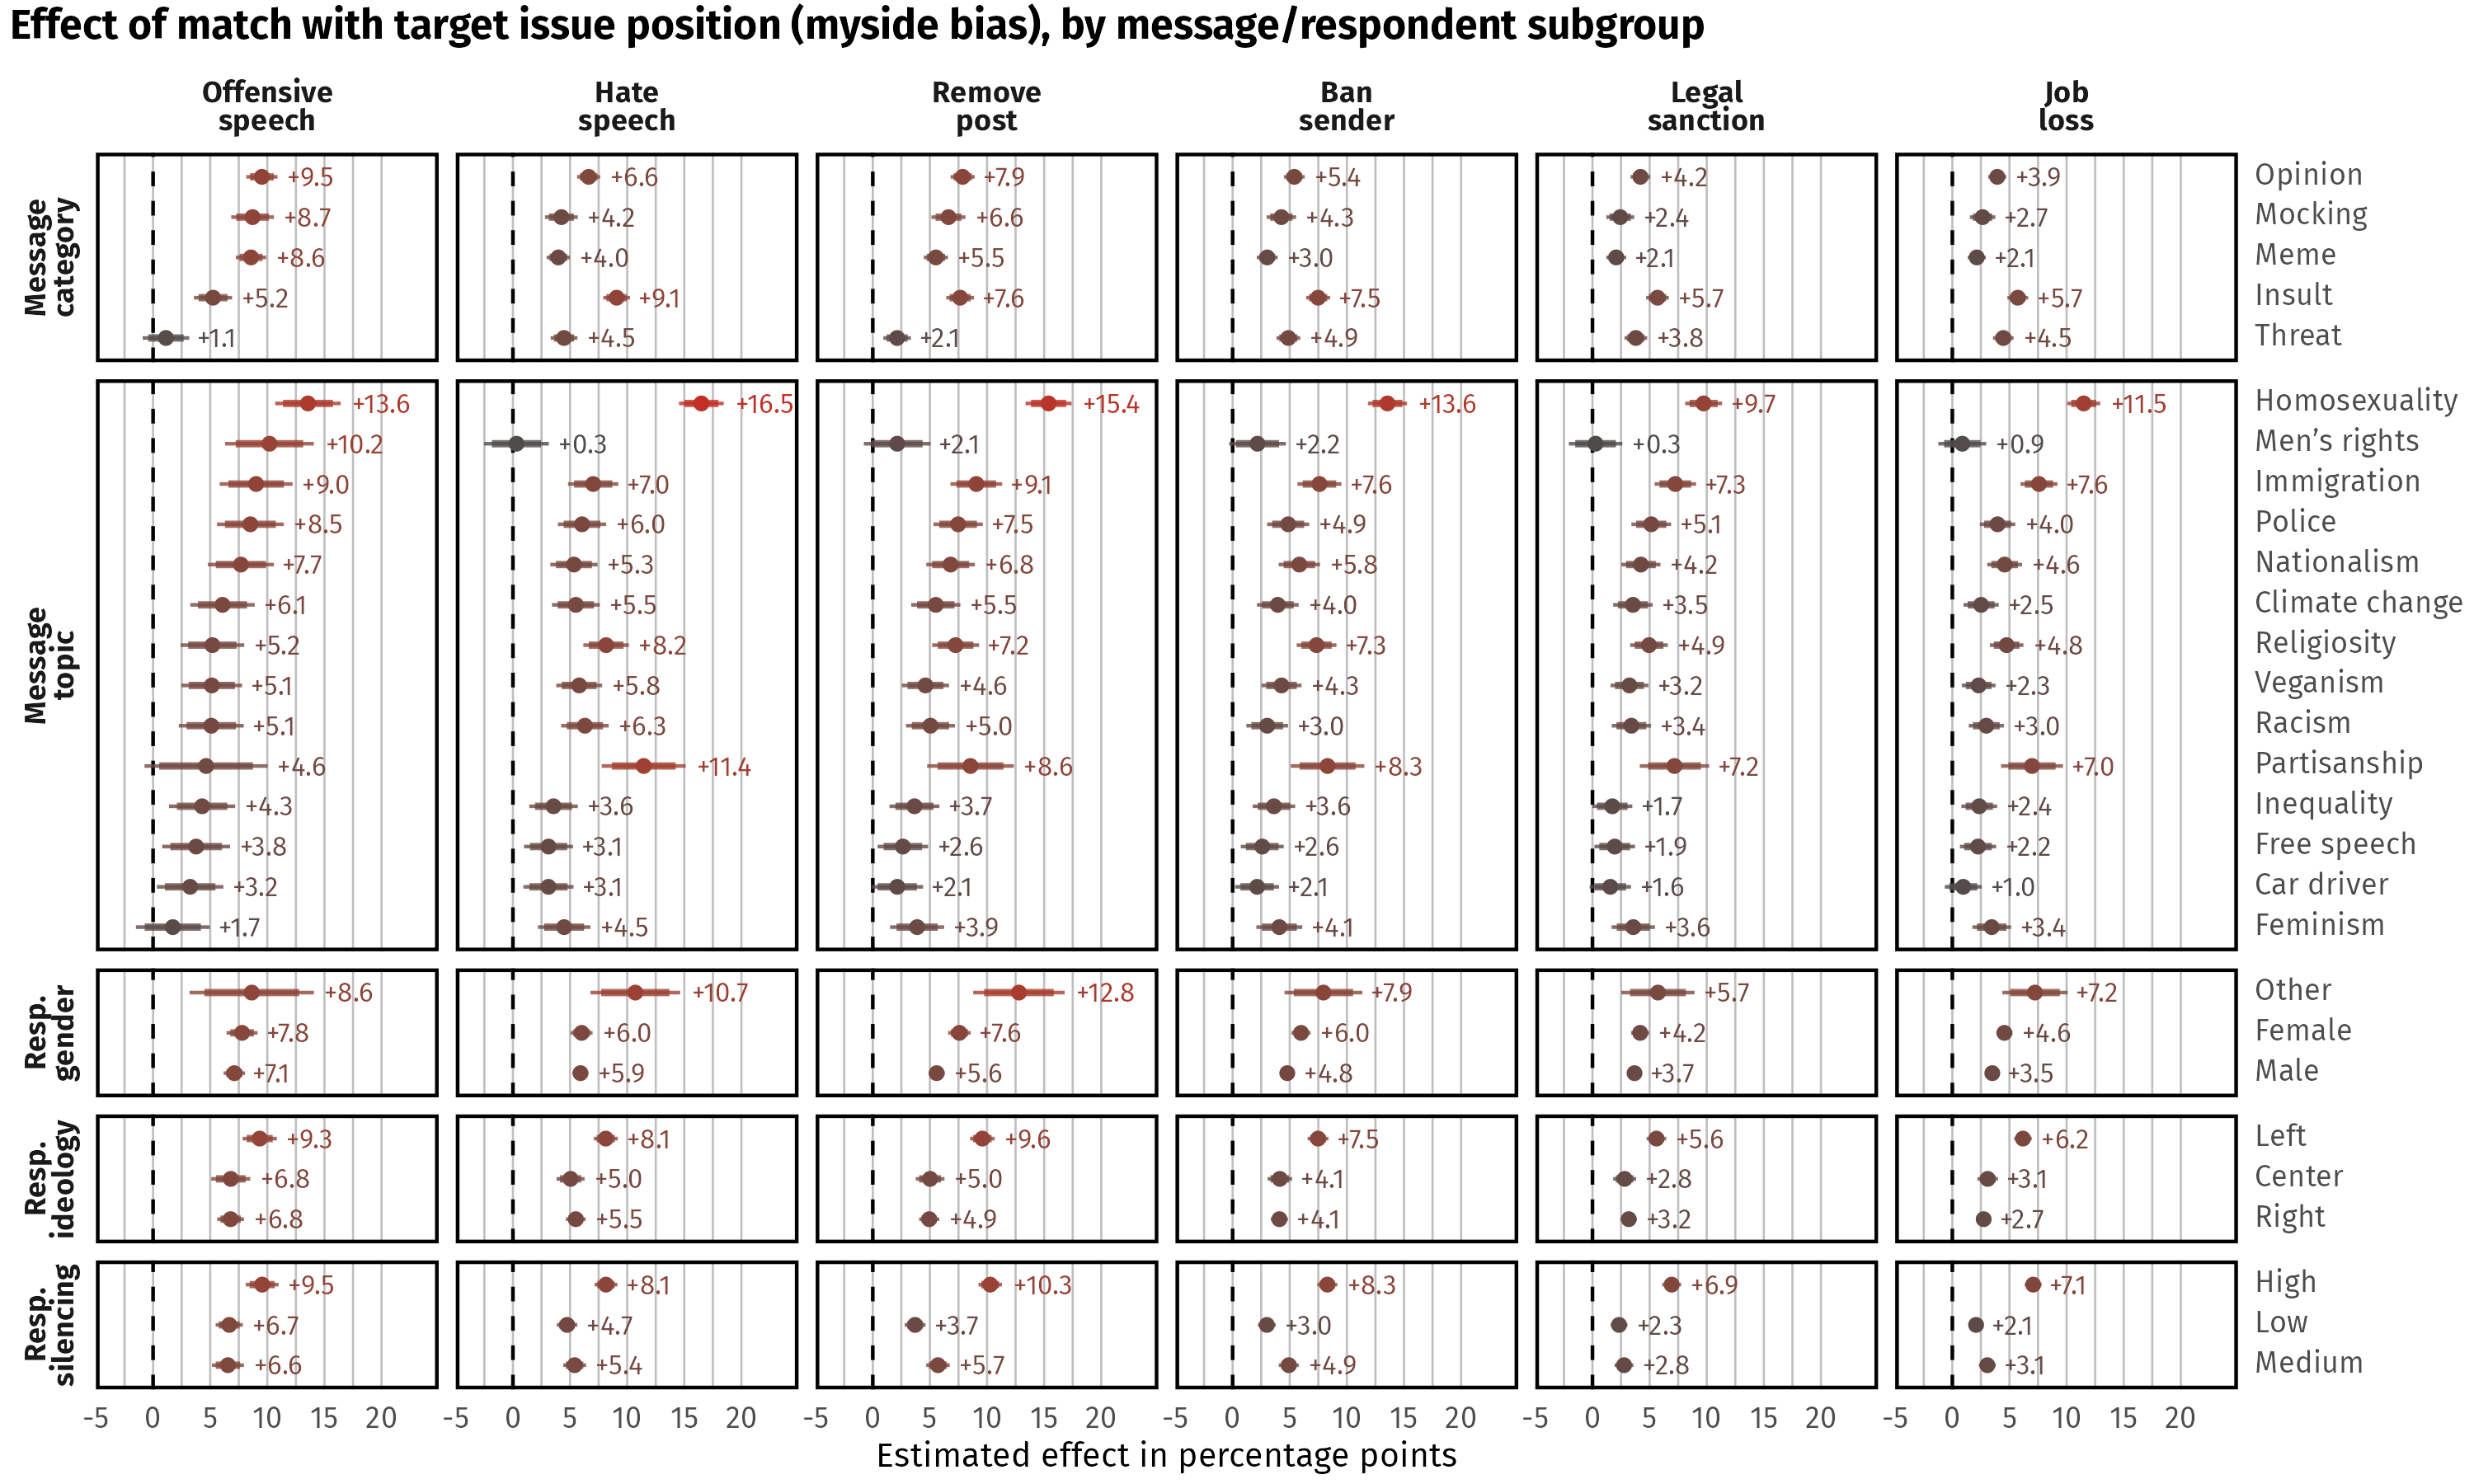
\includegraphics[width=1\linewidth]{figures/effects-h1-coefplot-heterogeneity.png}
\caption{\textbf{Variation in myside bias across speech types and respondent characteristics.} Estimates from hierarchical linear probability models with respondent, vignette deck, and country random effects. Each point represents the percentage-point difference in outcome probability for issue-stance alignment with the target compared to misalignment, estimated separately by message type or severity (left panels) and respondent subgroup (right panels). Respondent subgroup analyses are exploratory. Horizontal lines show 95\% and 99\% confidence intervals.}
\label{fig:effects-h1-coefplot-heterogeneity}
\end{figure}

%---------- DISCUSSION ------------%
\section*{Discussion}

% theoretical contribution
Our results establish myside bias as a structurally distinct and particularly intractable source of disagreement in content moderation. Prior work has documented that demographic characteristics of annotators---their gender, ethnicity, and partisanship---shape how they classify toxic speech~\cite{sapAnnotatorsAttitudesHow2022,dasInvestigatingAnnotatorBias2024,appelPartisanConflictContent2023}. Our findings extend this picture in a consequential direction: the strongest and most consistent predictor of moderation judgments is not who the moderator is but what they believe. This pattern is not confined to one political camp---respondents on both the left and the right are affected---and it holds for platform sanctions and offline consequences alike, as well as for both perception of offensiveness and willingness to sanction. These findings are consistent with motivated reasoning accounts of myside bias~\cite{stanovichBiasThatDivides2021,stanovichNaturalMysideBias2007}, though we acknowledge that the design cannot distinguish between motivated cognitive distortion and genuine normative disagreement about harm: respondents who share a target's position may genuinely believe attacks on it are more harmful, not merely perceive them as such for self-serving reasons. The practical implication for moderation systems, however, is the same under either account, and we return to this below.

% link to other research
Our results also confirm a finding from prior experimental work~\cite{munzertCitizenPreferencesOnline2025,pradelToxicSpeechLimited2024}: perceptions of speech and preferences for sanctions, while correlated, are distinct. Support for removing non-hateful content is low across all countries, and even threatening content fails to yield consensus for removal. This tolerance for contentious speech is a substantively important finding that sits alongside the myside bias result: people do not simply endorse broad censorship, but they do apply asymmetric standards depending on whose side is being attacked.

% limitations of aggregation-based approaches
A central implication of these findings concerns the limits of aggregation-based approaches to content moderation. Systems like Community Notes are designed around a bridging algorithm that requires cross-ideological agreement before a note is displayed, explicitly to guard against partisan bias~\cite{allenBirdsFeatherDont2022}. Recent evidence suggests these systems struggle with politically contentious content~\cite{renaultRepublicansAreFlagged2025,bouchaudAlgorithmicResolutionCrowdsourced2025}. Our results offer a specific mechanism: myside bias is not a function of partisan identity but of issue-stance alignment, which shifts dynamically across topics. A note criticizing an anti-immigration post may achieve cross-ideological consensus among respondents who happen to agree on that particular issue, while a note on a climate post fails for a differently configured set of reasons. Because the contours of disagreement vary issue by issue rather than tracking stable partisan or demographic fault lines, no fixed correction factor---demographic reweighting, annotator balance, or cross-ideological aggregation---can fully account for it. This does not mean that aggregation approaches are without value; it means that their effectiveness will be uneven across topics and contexts in ways that are difficult to predict or audit. Standard debiasing approaches calibrated on demographic or partisan dimensions will systematically miss the content-contingent component of disagreement that myside bias produces.

% policy implications
These findings suggest several concrete directions for platforms, regulators, and researchers. First, audits of annotation pipelines and model outputs should extend beyond demographic and partisan disparities to include myside-sensitive variation---assessing whether classification rates shift systematically with the political content of the speech being evaluated~\cite{sapAnnotatorsAttitudesHow2022,webbwilliamsWhenConservativesSee2023}. Second, majority-vote labeling schemes should be replaced or supplemented with disagreement-aware approaches that surface rather than suppress annotator disagreement, such as composite labels that encode the distribution of human judgments rather than collapsing it to a single ground-truth category~\cite{gordonJuryLearningIntegrating2022,webbwilliamsWhenConservativesSee2023}. Third, enforcement thresholds should be calibrated to the actual distribution of public tolerance across contexts rather than presuming uniform support for removal~\cite{atrejaRemoveReduceInform2023}; our results show that even for speech classified as hateful, many respondents decline to endorse sanctions, and this pattern varies substantially across countries and topics. Fourth, moderation policies should be localized to the cultural and legal contexts in which they operate, given that perceptions of harm and offensiveness demonstrably diverge across the countries we studied~\cite{jiangUnderstandingInternationalPerceptions2021,davaniDisentanglingPerceptionsOffensiveness2024}. These adjustments do not resolve the underlying normative question---whose values content moderation algorithms should represent and whose voices they should amplify~\cite{gordonJuryLearningIntegrating2022,webbwilliamsWhenConservativesSee2023}---but they shift the design of these systems from one that assumes a single objective standard toward one that acknowledges and accommodates the pluralism that our data reveal.

% limitations
Several limitations warrant caution. Our stimulus set, while broader than most prior work, does not fully represent the range of toxic speech that circulates on live platforms; for ethical reasons, we excluded the most extreme dehumanizing content, and our sample skews toward contentious rather than innocuous speech. The cross-national comparisons of baseline classification rates should be interpreted as descriptive rather than precise population estimates, given that our platform-recruited samples are non-probability samples that overrepresent younger, more educated, and more online-engaged respondents relative to national populations---a pattern that may be especially consequential for outcomes adjacent to the recruitment topic. Our measure of identity bias relies on stylized cartoon avatars, which provide weaker identity signals than photographs or named profiles; the null findings for gender and ethnicity overlap should be understood as null findings under this conservative operationalization rather than as evidence that identity bias is entirely absent in real moderation contexts. Finally, the heterogeneity findings---particularly the pattern of somewhat stronger myside bias among left-leaning respondents---are exploratory and should be interpreted with appropriate caution given the challenges of comparing ideological self-placement across eleven politically diverse countries. Future work should address these limitations with richer identity cues, anchoring vignettes to support cross-national comparisons, and platform-based field experiments that test whether the disagreement-aware interventions we recommend actually reduce myside-sensitive inconsistency in practice.

% closing
Content moderation at scale requires human judgment, and human judgment about contested speech is inescapably tied to what people believe. Treating this as a technical calibration problem---to be solved by better classifiers or larger annotation pools---misses the point. The challenge is political: it concerns whose standards of harm should govern shared online spaces. Acknowledging that challenge explicitly, and building moderation systems that surface disagreement rather than papering over it, is a more honest and ultimately more legitimate path forward.


%%%%%%%%%%%%%%%% MAIN TEXT FIGURES %%%%%%%%%%%%%%%


\section*{Materials and Methods}

This research was approved by the Research Ethics Committee at the Hertie School (application no. 2022-10-24-04) and pre-registered at OSF prior to data collection on November 16, 2022 (\url{https://osf.io/2ec8m}). Pre-registered hypotheses and all deviations from the pre-analysis plan are documented in SI section~\ref{si:pap}.

\subsection*{Participants}

Between November 21 and December 30, 2022, we recruited participants in 11 countries: Brazil, Colombia, Germany, India, Indonesia, Nigeria, the Philippines, Poland, Turkey, the United Kingdom, and the United States. Participants were recruited via targeted advertisements on Facebook and Instagram, following established practices for platform-based survey recruitment~\cite{neundorfHowImproveRepresentativeness2023}. This approach yields non-probability samples that overrepresent younger, more educated, and more online-engaged respondents relative to national populations; sample composition by country is documented in SI section~\ref{si:recruitment}. We excluded respondents who completed the survey in under five minutes (pre-registered exclusion rule; median completion time: 19.5 minutes), leaving a final sample of 19,172 participants. Speeder exclusion rates did not differ meaningfully across experimental conditions, supporting the assumption that the exclusion was non-differential with respect to treatment assignment (SI section~\ref{si:recruitment}).

The survey was translated into the official languages of each country by native speakers familiar with the respective country contexts. In addition to an English version, we fielded a Hindi version in India and a Filipino version in the Philippines. Links to all questionnaires are provided in SI section~\ref{si:questionnaire}.

Participants provided informed consent at the start of the survey. Before the vignette task, they received a content warning and were given the option to skip any items that might be distressing.

\subsection*{Experimental setup}

The survey design comprised three independently randomized components. The primary component was the vignette-based conjoint experiment. After completing background questions about their characteristics, attitudes, and behaviors, respondents evaluated eight synthetic social media conversations sequentially, each paired with the outcome measures described below.

Each conversation depicted a sender responding to a target's post. Vignette attributes spanned target and sender characteristics (gender, apparent ethnicity, and --- for the target --- issue stance) and message features (topic, speech type, and severity). All attribute levels were independently randomized. Each respondent was assigned one of 400 pre-constructed vignette decks, balanced so that each deck contained equal numbers of left- and right-leaning target positions, equal numbers of male and female senders and targets, and a representative spread of speech types and severity levels. Sender and target ethnicity were oversampled to match the modal ethnicity in each country sample. All vignette stimuli were generated by the research team and adapted to country context by supervised native-speaker translators; full stimulus materials are provided in SI section~\ref{si:vig-construction}.

The two additional pre-registered experimental components---a framing experiment varying the platform context in which the moderation task was presented, and a question-order experiment testing short-term effects of toxic speech exposure on governance preferences---are described and their results reported in SI sections~\ref{si:exp-setup} and~\ref{si:addresults}.

\subsection*{Outcome measures}

For each vignette, respondents evaluated the sender's message on six binary outcomes. The perception item asked whether the message constituted hate speech, offensive-but-not-hate speech, or neither; we treat this trichotomy as two binary outcomes (hate speech vs. not; offensive-or-worse vs. neither). The four action items asked, in binary format, whether the post should be removed from the platform, whether the sender should be banned, whether the sender should face legal consequences such as a fine, and whether the sender should face consequences from their employer such as being fired. Exact item wording and survey screenshots are provided in SI section~\ref{si:measurement}.

\subsection*{Covariates and indices}

We measured respondent characteristics across four domains: sociodemographics (gender, age, education, ethnicity, minority status); political orientations (political interest, left-right ideology); psychological dispositions (empathy, belief in the importance of silencing others); and self-reported online behavior (exposure to toxic speech, hostile engagement online, speech regulation attitudes). Partisanship was measured but could not be harmonized across country samples and was therefore excluded from the models, as documented in the pre-analysis plan deviations (SI section~\ref{si:pap}). Multi-item constructs were reduced to composite scores via principal components analysis; variable processing and index construction are detailed in SI section~\ref{si:measurement}.

\subsection*{Statistical analyses}

We analyzed the vignette experiment using hierarchical linear probability models with random intercepts for respondents, vignette decks, and countries (in pooled analyses). Respondent-level random intercepts account for the nesting of eight vignette evaluations within each respondent; vignette-deck random intercepts adjust for deck-specific variation. Linear probability models allow coefficients to be interpreted directly as percentage-point differences in outcome probabilities.

A formal power analysis using the formula of~\cite{schuesslerPowerAnalysisConjoint2020} indicates that, given this sample size, we can detect average marginal component effects as small as 5 percentage points with power of 1.0 at $\alpha = 0.05$. Myside bias is estimated as an interaction between issue-stance alignment and vignette attributes, which requires greater power; we can nonetheless detect interaction effects of 4 percentage points with power of 0.84 at $\alpha = 0.05$ in the pooled sample. Country-specific samples are less well powered for interaction detection, particularly Nigeria; country-level interaction estimates should be interpreted with appropriate caution (SI section~\ref{si:power}).

All analyses follow the pre-registered analysis plan. We use two-tailed tests and a significance threshold of $p < .05$. Missing values are handled by model-specific listwise deletion. In line with the pre-analysis plan, we report results from several additional analyses in SI section~\ref{si:addresults}, including exploratory heterogeneity analyses. These include models that are run only using content moderation decisions for which respondents spent at least 5 seconds on the respective page as well as country-specific results of the main models. Furthermore, we report results from the two additional experiments that were pre-registered. We do not apply population weights for experimental effect estimates, as random assignment protects internal validity under modest demographic imbalance~\cite{miratrixWorthWeightingHow2018,gerber_green_2012}. For descriptive statistics reported in the SI, we apply country-specific weights that post-stratify on sex-by-age distributions and rake to national education marginals.






%%%%%%%%%%%%%%%% REFERENCES %%%%%%%%%%%%%%%

\clearpage % Clear all remaining figures and tables then start a new page

% The list of references goes after the main text and before the acknowledgements
% When preparing an initial submission, we recommend you use BibTeX, like this:
%
\bibliography{references.bib} % for a file named science_template.bib
\bibliographystyle{sciencemag}



%%%%%%%%%%%%%%%% ACKNOWLEDGEMENTS %%%%%%%%%%%%%%%

% --------------------------------- %
\section*{Acknowledgments}

We thank the participants of our study for their engagement. We are grateful to our translators, and to Sebastian Ramirez Ruiz for their research assistance. We also thank participants of the Political Economy Lunch Seminar at the Hertie School, the Workshop on Content Moderation, Free Speech and Platform Governance at Royal Holloway, University of London, and the CIVICA Youth Gender Polarization and Digital Fragmentation Conference at the European University Institute for their helpful suggestions. We acknowledge the support of this project through an unrestricted gift by Facebook Core research.

\paragraph*{Funding:} 
This research was funded by Facebook Core Research as part of the Content Governance Request for Proposals 2019 (S.M.). The funder had no role in study design, data collection and analysis, decision to publish, or preparation of the manuscript. Conclusions, or recommendations presented in this material are solely those of the authors and do not necessarily represent the views of the funder.

\paragraph*{Author contributions:} 
Conceptualization and study design: S.M., J.E., L.O., R.T.; Methodology: S.M., R.T.; Data collection: S.M., J.E., L.O.; Data analysis: S.M.; Funding acquisition: S.M., R.T.; Project administration: S.M., J.E., L.O.; Supervision: S.M.; Writing – original draft: S.M.; Writing – review and editing: S.M., J.E., L.O., R.T.

\paragraph*{Competing interests:} 
The authors declare no competing interests.

\paragraph*{Data and materials availability:}
The preregistration, study materials, R scripts, and anonymized replication data are publicly accessible through the Open Science Framework (OSF) at \url{https://osf.io/2ec8m}.

%%%%%%%%%%%%%%%% END OF MAIN TEXT %%%%%%%%%%%%%%%

\newpage

%%%%%%%%%%%%%%%% START OF SUPPLEMENT %%%%%%%%%%%%%%%

\clearpage
\normalsize
\onecolumn

\begin{appendices}
  \renewcommand\thetable{\thesection\arabic{table}}
  \renewcommand\thefigure{\thesection\arabic{figure}}
 \setcounter{figure}{0}  
 \setcounter{table}{0}
 \setcounter{page}{1}
\thispagestyle{plain}


\begin{center}
\section*{Supplementary Materials for\\ \scititle}

% Author list for the supplement
% Indicate the corresponding authors, but do NOT include institutions here
% It would be nice if the template auto-generated this, but doing so is complicated...
Simon Munzert$^{\ast}$,
Julia Ellingwood,
Lisa Oswald,
Richard Traunmüller\\ % we're not in a \author{} environment this time, so use \\ for a new line
	\small$^\ast$Corresponding author. Email: munzert@hertie-school.org\\
\end{center}

\setstretch{1.1} 
\tableofcontents
\setstretch{1.1} 

%%%%%%%%%%%%%%%% MATERIALS AND METHODS %%%%%%%%%%%%%%%

\clearpage

% --------------------------------- %
\clearpage
\section{Supplementary Text}


\subsection{Pre-Analysis Plan and Deviations}\label{si:pap}

The study was pre-registered at OSF prior to data collection on November 16, 2022. The pre-registration and pre-analysis plan is available here: \url{https://osf.io/2ec8m}.

\subsubsection{Hypotheses}

\begin{enumerate}
    \item \textbf{Speech-respondent interactions (issue-based myside bias and in-group identity bias)}
    \begin{itemize}
        \item \textbf{H1:} Respondents who agree (vs. disagree) with the issue position of the target are more likely to perceive messages as being hate speech and offensive speech, and to prefer platform, legal, and employer action against the message/sender.
     \item \textbf{H2:} Respondents who share gender or ethnicity with the target are more likely to perceive messages as being hate speech and offensive speech, and to prefer platform, legal, and employer action against the message/sender.
        \item \textbf{H3:} Respondents who share gender or ethnicity with the sender are less likely to perceive messages as being hate speech and offensive speech, and to prefer platform, legal, and employer action against the message/sender.
    \end{itemize}
    \item \textbf{Framing experiment (sensitivity of moderation in different contexts)}
    \begin{itemize}
        \item \textbf{H4:} If the vignette evaluation is framed as a moderation task for a platform that promotes free speech and takes a critical stance against any form of censorship (vs. a neutral frame), respondents are less likely to prefer platform action against the message sender but are as likely to perceive messages as being hate speech and offensive speech, and to prefer legal action against the message/sender.
        \item \textbf{H5:} If the vignette evaluation is framed as a moderation task for a platform that vows to protect vulnerable users from hate speech and takes an aggressive stance against hateful content on their pages (vs. a neutral frame), respondents are more likely to prefer platform action against the message sender but are as likely to perceive messages as being hate speech and offensive speech, and to prefer legal action against the message/sender.
    \end{itemize}
    \item \textbf{Question order experiment (exposure effects of toxic speech)}
    \begin{itemize}
    \item \textbf{H6:} If respondents are exposed to the vignette evaluation task before (vs. after) they get to answer questions about governance of speech, they are more willing to have speech restricted, and see more responsibility for action against hate speech in the hands of online services, lawmakers, the justice system, and employers.
    \end{itemize}
\end{enumerate}


\subsubsection{Deviations}

Although the results we present here are based on the pre-analysis plan we registered prior to obtaining the data (see details at \url{https://osf.io/2ec8m}), there were a few areas in which we had to deviate from the plan. For the sake of transparency, we report each of these deviations here:

\begin{enumerate}
    \item \textbf{Recruitment:} The pre-registration of this study specified a target of at least 1,500 respondents per country. This target was not met for a subset of countries (see SI section~\ref{si:recruitment}). However, this shortfall was offset by relatively higher numbers of respondents in a few other countries, resulting in an average of approximately 1,740 respondents per country.
    \item \textbf{Recruitment:} The pre-registration stated: “We will use targeting based on age (18–40 and 41–65+), sex (male, female), and education (below college, at least college education) where necessary to attain a sample that is balanced on the marginals across those categories.” In practice, we only targeted two age groups within each country. 
    \item \textbf{Measurement:} We operationalized ethnicity as \emph{white/non-white} by pooling all non-white avatar categories. The avatars were designed to signal broad ethnic appearance through skin tone and facial features, but respondents' avatar selections did not reliably correspond to the ethnic category the research team had assigned to each avatar---a pattern that was especially pronounced in non-Western samples where the ``Arabic'' and ``South Asian'' avatar sets were selected by respondents across multiple countries in ways that did not match national majority groups (see SI section~\ref{si:vig-construction}). Skin tone therefore served as the more operationally reliable basis for defining ethnic in-group membership, and we classified only the four lightest-skinned avatars as ``white.'' This operationalization represents a conservative and imperfect proxy for ethnic identity; the null findings for ethnicity overlap should be interpreted accordingly.
    \item \textbf{Measurement:} Political partisanship was not included as a covariate in the models because it could not be harmonized across country samples.
    \item \textbf{Measurement:} For the construction of the \emph{experience of online hate} and \emph{hostile engagement online} measures, continuous scores were divided into three categories—Low, Medium, and High—based on tertiles of the score distribution (0–33rd, 34th–66th, and 67th–100th percentiles). This deviates from the pre-analysis plan, which had specified the use of average scores across items. We opted for the categorical specification to maintain consistency with other covariates.
    \item \textbf{Modeling:} We included vignette position as a control variable in all models. We did so because vignette position demonstrably affects moderation preferences, and controlling for it helps to reduce noise in the models.
    \item \textbf{Modeling:} For the analyses of the framing and the exposure experiments, we decided not to include the covariate adjustment based on \cite{linAgnosticNotesRegression2013}, even though it was pre-registered, because the adjustment did not materially change the results and added unnecessary model complexity. Given that randomization was successful and covariates were balanced across conditions, the unadjusted estimates provide a clear presentation of the treatment effect without affecting inference.
    \item \textbf{Analysis:} We did not analyze the open-ended responses at the end of the survey for this study; those findings will be reported in a separate paper.
\end{enumerate}


% --------------------------------- %
\clearpage
\subsection{Participant Recruitment}\label{si:recruitment}

\subsubsection{Recruitment strategy}

Between November 21 and December 30, 2022, we recruited participants in 11 countries: Brazil, Colombia, Germany, India, Indonesia, Nigeria, the Philippines, Poland, Turkey, the United Kingdom, and the United States. We selected those countries to capture broad global variation in cultural, political, and socio-technical contexts relevant to online speech and content moderation. These countries collectively represent major world regions, different stages of economic development, and a wide range of internet governance regimes and democratic institutions. Prior work shows that perceptions of harmful or offensive content vary substantially across cultural and moral contexts \cite{davaniDisentanglingPerceptionsOffensiveness2024} and that moderation norms are shaped by local political and legal traditions \cite{jiangUnderstandingInternationalPerceptions2021,aroraDetectingHarmfulContent2023a}. The country set covers high- and middle-income democracies (e.g., the U.S., U.K., Germany, Brazil, India) and emerging markets with large online populations (e.g., Indonesia, Nigeria, the Philippines), thereby balancing cultural diversity and practical relevance for global platforms. Platform-based recruitment via Meta Ads produces non-probability samples that systematically overrepresent users who are younger, more educated, more politically engaged, and more active online than national adult populations. The demographic composition of each country sample relative to population benchmarks is documented in the Sample Demographics subsection below. For experimental contrasts, these imbalances do not threaten internal validity because treatment was randomized; for descriptive cross-national comparisons, they should be treated as a source of potential confounding.


Participants were recruited using Meta Ads delivered on both Facebook and Instagram. We used targeting based on age (18-40 and 41-65+ years). We promoted ads as posts of public profiles ``The Digital Citizen Lab” (Facebook) ``digitalcitizenlab'' (Instagram), both created and managed by us. Following recommendations of \cite{neundorfHowImproveRepresentativeness2023}, we optimized ad delivery on respondents completing the survey. We selected ``highest volume'' as campaign bid strategy and used Advantage+ placements. The audiences consisted of people living in the respective country, speaking the language to which the survey and ad had been translated.

\subsubsection{Translation}

The questionnaire was first developed in English and then translated into the main languages spoken in the participating countries to ensure clarity and cultural appropriateness. In India, the survey was administered in both English and Hindi, while in the Philippines it was available in English and Filipino. The translation process followed a collaborative and iterative approach: native speakers from each country worked closely with the research team to produce accurate and contextually appropriate translations. These translations were then checked through a back-translation procedure, in which independent bilingual speakers retranslated the materials into English to verify semantic consistency and resolve discrepancies. This process helped ensure that all versions of the questionnaire conveyed the same meaning across languages and cultural contexts. Links to all questionnaires are provided in SI section~\ref{si:questionnaire}.

\subsubsection{Ad design}

We used two different ad versions (see Fig.~\ref{fig:fb-ads}). The neutral ad consisting of the text ``Do you want to participate in our survey? Hertie School researchers want to hear your opinions." and a neutral image of two pencils. A second ad consisted of the text ``What should people be allowed to say on social media? Hertie School researchers want to hear your opinions." and an image of a stop signaling hand in front of face (ad texts were translated for non-English audiences). The images used are in the public domain (published under the free \href{https://unsplash.com/license}{Unsplash license}, which is broadly equivalent in scope to the Creative Commons Zero (CC0) license) and were kept constant during the entire time of the campaign. Once participants clicked on the ``learn more" action button in the advertisement, they were directed to our survey, hosted on a Qualtrics page. 

\begin{figure}[t!]
\begin{center}
\includegraphics[width=0.49\textwidth]{figures/facebook-ad-neutral.png}
    \includegraphics[width=0.49\textwidth]{figures/facebook-ad-topic.png}
\caption{\textbf{Recruitment ads.} Neutral ad (left) was headed by the statement ``Hertie School researchers want to hear your opinions! Do you want to participate in our survey?" whereas the topic-specific ad (right) was headed by the statement ``Hertie School researchers want to hear your opinions! What should people be allowed to say on social media?".}
\label{fig:fb-ads}
\end{center}
\end{figure}

The ads were favored very differently by the targeting algorithm. The topic-specific version was more effective in attracting people to the survey for both targeted age demographics (see Table~\ref{tab:survey-adtype-pooled}). about 82\% of all completed interviews were recruited via the topic ads. The topic ad was the more popular one in all countries (see Table~\ref{tab:survey-adtype}), although the shares vary between 51\% (Colombia) and 96\% (United Kingdom). 

\input{figures/survey-adtype-pooled.tex}

\input{figures/survey-adtype.tex}


\subsubsection{Data collection}

Data was collected from November 24, 2022 to December 30, 2022. Before starting the survey, participants were informed about the length, objectives, and risks of the survey and asked to provide explicit informed consent. Furthermore, participants were debriefed at the end of the survey. Following the pre-analysis plan, we excluded speeders from the analyses, whom we defined as participants who spent less than five minutes on the entire survey (the median survey taking time was 19.5 minutes; see Table~\ref{tab:survey-completion-times}). This left us with a sample of 19,172 participants.

\input{figures/survey-completion-times.tex}

Recruitment success varied across countries. For some, the targeted sample size of 1,500 per country was reached quickly, whereas for others that target was not reached by the end of the field period (i.e. when the budget ran out). Figure~\ref{fig:lineplot-recruitment-respondents} provides an overview of the cumulative number of survey respondents over time, by country. In the middle of the campaign, we started to prioritize countries with low completion totals, which were also the more costly interviews. 

Completion rates varied significantly, from less than 18\% (Philippines) to over 67\% (see Table~\ref{tab:survey-attrition}). We count as completed every respondent who gave consent, spent at least 5 minutes on the interview, and completed more than 93\% of the interview, which covered all substantively relevant questions. The completion rate is computed as the share of completed interviews among all who clicked the survey link and landed on the Qualtrics server. 

Low completion rates are correlated with higher costs per interview (see Table~\ref{tab:survey-costs}). The budget spent on each country sample varied significantly, as did the costs per completed interview (CPI). The cheapest interviews were realized in the United Kingdom (EUR 0.93), the most expensive ones in Nigeria (EUR 6.15). 

\begin{figure}[t!]
\begin{center}
\includegraphics[width=1\textwidth]{figures/lineplot-recruitment-respondents.png}
\caption{\textbf{Cumulative number of survey respondents over time, by country.} Number of completed interviews reported. Field time: November 24, 2022 to December 30, 2022.}
\label{fig:lineplot-recruitment-respondents}
\end{center}
\end{figure}

\input{figures/survey-attrition.tex}

\input{figures/survey-costs.tex}

Country targeting appears to have been largely successful. Based on geolocated IP addresses automatically provided by the survey software, the vast majority of respondents are located in the intended target country (see Fig.~\ref{fig:map-respondent-locations}).

\begin{figure}[t!]
\begin{center}
\includegraphics[width=1\textwidth]{figures/map-respondent-locations.png}
\caption{\textbf{Respondent locations based on geolocations of device IPs}}
\label{fig:map-respondent-locations}
\end{center}
\end{figure}


\clearpage
\subsubsection{Sample demographics}

We summarize here the basic demographics of our survey samples and compare them to corresponding population benchmarks. Population statistics on sex–age distributions are taken from the United Nations World Population Prospects 2022 dataset \cite{desa2022united}. Population statistics on educational attainment were gathered from the UNESCO Institute for Statistics and World Bank Education Data \cite{unesco_uis_api} and harmonized with our three-level education classification. 

Across all country samples, we observe substantial deviations from population marginals (see Fig.~\ref{fig:demographics-set1} and~\ref{fig:demographics-set2}). Respondents in our surveys tend to be disproportionately male, younger, and more highly educated than the general adult population—a pattern consistent with well-documented selection effects in online recruitment, including those observed for Meta/Facebook Ads samples \cite{neundorfHowImproveRepresentativeness2023,zhangQuotaSamplingUsing2020}. These imbalances should be kept in mind when interpreting descriptive statistics, as they may shape raw point estimates. Beyond descriptive baselines, the recruitment method may also affect experimental effect sizes if the sample systematically overrepresents respondents with strong prior attitudes toward online speech moderation---a group that is plausibly more likely to respond to platform-based speech-related advertising. The direction and magnitude of any such bias is unknown; we flag it as a limitation rather than a correction.

For our experimental analyses, we follow our pre-analysis plan and do not apply population weights. Random assignment protects the internal validity of experimental contrasts, and demographic imbalance does not generally bias treatment effect estimates when treatment is randomized \cite{miratrixWorthWeightingHow2018,gerber_green_2012,deaton_cartwright_2018}. We therefore expect limited substantive impact of sample–population deviations on the causal quantities of interest.

For descriptive evidence reported in the supplementary materials, we construct demographic population weights in two steps. Full post-stratification is not feasible because sex × age × education joint distributions are unavailable for many contexts. Therefore, we first post-stratify on sex–age cells using UN population figures. We align age categories with those for which internationally comparable benchmarks are available. Second, we apply iterative proportional fitting (raking) to match national marginals of the ISCED education brackets.


\begin{figure}[htb]
\centering
% --- Row 1 ---
\begin{subfigure}{0.44\textwidth}
  \centering
  \includegraphics[width=\linewidth]{figures/demographics-bra.png}
  \caption{\centering Brazil}
\end{subfigure}
\hfill
\begin{subfigure}{0.44\textwidth}
  \centering
  \includegraphics[width=\linewidth]{figures/demographics-col.png}
  \caption{\centering Colombia}
\end{subfigure}
% --- Row 2 ---
\begin{subfigure}{0.44\textwidth}
  \centering
  \includegraphics[width=\linewidth]{figures/demographics-ger.png}
  \caption{\centering Germany}
\end{subfigure}
\hfill
\begin{subfigure}{0.44\textwidth}
  \centering
  \includegraphics[width=\linewidth]{figures/demographics-gbr.png}
  \caption{\centering Great Britain}
\end{subfigure}
% --- Row 3 ---
\begin{subfigure}{0.44\textwidth}
  \centering
  \includegraphics[width=\linewidth]{figures/demographics-ind.png}
  \caption{\centering India}
\end{subfigure}
\hfill
\begin{subfigure}{0.44\textwidth}
  \centering
  \includegraphics[width=\linewidth]{figures/demographics-idn.png}
  \caption{\centering Indonesia}
\end{subfigure}
\caption{\textbf{Sample vs. population demographics}}
\label{fig:demographics-set1}
\end{figure}


\begin{figure}[htb]
\centering
% --- Row 1 ---
\begin{subfigure}{0.44\textwidth}
  \centering
  \includegraphics[width=\linewidth]{figures/demographics-nig.png}
  \caption{\centering Nigeria}
\end{subfigure}
\hfill
\begin{subfigure}{0.44\textwidth}
  \centering
  \includegraphics[width=\linewidth]{figures/demographics-phl.png}
  \caption{\centering Philippines}
\end{subfigure}
% --- Row 2 ---
\begin{subfigure}{0.44\textwidth}
  \centering
  \includegraphics[width=\linewidth]{figures/demographics-pol.png}
  \caption{\centering Poland}
\end{subfigure}
\hfill
\begin{subfigure}{0.44\textwidth}
  \centering
  \includegraphics[width=\linewidth]{figures/demographics-tur.png}
  \caption{\centering Turkey}
\end{subfigure}
% --- Row 3 ---
\begin{subfigure}{0.44\textwidth}
  \centering
  \includegraphics[width=\linewidth]{figures/demographics-usa.png}
  \caption{\centering United States}
\end{subfigure}
\hfill
\begin{subfigure}{0.44\textwidth}
  \centering
  \vspace{1.2cm}
  \caption*{}
\end{subfigure}
\caption{\textbf{Sample vs. population demographics}, \emph{continued}}
\label{fig:demographics-set2}
\end{figure}





% --------------------------------- %
\clearpage
\subsection{Construction of social media posts}\label{si:vig-construction}

\subsubsection{Vignette design and attributes}

At the core of our experiment, respondents evaluate brief social media conversations between a target and a sender who comments on the target’s post. This section describes how those conversations were constructed. Importantly, all content elements were generated by us to ensure full control over every feature.

The social media posts were designed to closely resemble exchanges on a popular social media platform (in this case, Facebook). Irrelevant interface elements such as timestamps, likes, or sharing options were omitted. Only features representing relevant vignette attributes were retained. These attributes capture issue content, as well as characteristics of the sender and target, and features of both the sender’s and target’s messages. Figure~\ref{fig:design-overview} in the main text provided an overview of the attributes that were used to generate the fictitious  conversations. The materials corresponding to the various attributes and levels are documented in detail in Section~\ref{si:posts}.

In the following, we outline the rationale behind creating the different parts, including the target posts, the sender responses, and both sender and target characteristics.

Furthermore, we provide an online interface through which all messages from all country samples can be interactively explored: \url{digital-citizen-lab.com/myside-bias-vignettes}.

\paragraph{Target message.} 
The target message constitutes the starting point of each vignette and is defined by two key dimensions: the issue under debate and the stance that the target expresses on that issue. Table~\ref{tab:target-messages} in SI Section~\ref{si:posts:targetmessages} provides a comprehensive overview of all target messages, organized by issue and stance category.

The target’s issue position serves as the central cue in our design, as it allows us to identify stance-based (``myside'') bias in participants’ moderation judgments. The set of 14 issues was selected to encompass a broad range of socially and politically salient topics that are, at least in some contexts, potentially polarizing or contentious. Each target statement was deliberately worded in a clear and pointed manner to minimize ambiguity regarding the expressed stance. 

As demonstrated by differences in support for these statements between left- and right-leaning respondents (see Fig.~\ref{fig:desc-issue-positions}), the messages effectively differentiate between ideological camps. This confirms that the vignettes capture attitudinal divides that are both realistic and theoretically meaningful, providing a strong foundation for studying how respondents evaluate and moderate content across political lines.

\paragraph{Sender message.}

The sender message lies at the heart of the moderation task: it is the component on which respondents are asked to focus when reporting their perceptions and moderation preferences. Most of the attributes included in our conjoint design refer specifically to variations in these messages. 

Table~\ref{tab:message-content-scheme} illustrates the rationale behind the different types of speech we employed to generate the content. In our design we distinguished four categories of speech acts: opinion/policy position, incivility/insult, threat/violence, mocking/sarcasm (including meme-based attacks). Each category (with the exception of mocking/sarcasm) was subdivided into two levels of severity—moderate and extreme. For the mocking/sarcasm category, we operationalized the two levels as distinct forms: a verbal mocking form and a visual meme-based form.

The selection of these four speech types is grounded in the literature on toxic language and hate speech, and reflects typologies commonly used in computational and social science research. 

First, \textit{opinion or policy positions} are included because much of the debate around hate speech and online toxicity revolves around the blurred line between expressing controversial opinions and promoting harmful ideologies. Such opinion expressions can serve as precursors or gateways to more explicit hostility, as noted in analyses of normative advocacy and ideological toxicity \cite{tirrellToxicSpeechEpidemiology2017}. Including these statements allows us to examine how participants respond not only to overt harassment but also to value-laden normative assertions that underpin polarized discourse.

Second, \textit{incivility and insult} form a foundational dimension of abusive online communication. Ad hominem attacks, name-calling, and ridicule are among the most frequent forms of interpersonal hostility observed on social media, undermining deliberative discourse and contributing to a hostile online climate. The pervasiveness of such incivility has made it a core category in toxic speech annotation taxonomies and moderation frameworks \cite{fortunaToxicHatefulOffensive2020}.

Third, \textit{threats and violent language} represent the most severe form of toxic speech, directly invoking or wishing physical harm. These expressions not only violate most platform policies but also overlap with legally recognized “true threats” in offline jurisprudence. In computational studies, threat language has been identified as a key linguistic marker of ``othering" and group-based hostility \cite{hartvigsen2022toxigen}.

Finally, \textit{mocking, sarcasm, and memes} capture the increasingly multimodal and indirect expressions of toxicity in online settings. Sarcasm and irony can mask aggression under humor, while memes—combining image and text—enable veiled and viral forms of hate speech that often evade detection \cite{martinezpandianiToxicMemesSurvey2025}. As \cite{martinezpandianiToxicMemesSurvey2025} argues, memes have become a distinctive communicative vehicle for the spread of ideological content. Here, this means that they are also used to circulate demeaning stereotypes or celebrate violence through ostensibly humorous content. Memes are not inherently tied to any single speech category, as they primarily describe a form of expression rather than a specific type of content. In our design, however, we restrict their use to content that falls within the category of \textit{mocking}.

Together, these four categories correspond to established taxonomies of hate and toxic speech that distinguish between normative, interpersonal, and threatening forms of communication \cite{kennedyIntroducingGabHate2022,mansurTwitterHateSpeech2023,pachingerDisambiguatingDefinitionsAbusive2023}. By systematically varying the type and severity of these speech acts, our design captures key facets of contemporary online hostility while preserving theoretical relevance and ecological validity.

To make levels of severity roughly comparable across categories and across topics, we specified for each category what “moderate” versus “extreme” would entail (see column ``Description") in Table~\ref{tab:message-content-scheme}. Furthermore, the speech acts were tailored toward each topic in order to increase ecological validity: we sought naturalistic phrasing that would plausibly appear in everyday social media conversations. At the same time, we recognize that this tailoring implies that perceptions of offensiveness or hatefulness may be influenced not only by the general features of the speech act but also by topic-specific content: for instance, a moderate insult targeted at a pro-immigration target might be perceived quite differently than one aimed at a pro-veganism target. Because our interest lies primarily in the effects of the other conjoint attributes (rather than topic-specific effects per se), we regard it as a strength of our design that we operationalized a wide variety of speech‐act types within and across topics.

We also made efforts to ensure comparability between group- and person-directed attacks within each category. Thus for example we might include “Stay-at-home moms are leeches on the system!” as a group attack, and “You are a leech on the system!” as a person-directed attack. As far as possible, attacks were exclusive in their categorization: that is, a threat/violence message avoided also using a clearly insulting slur, so as not to inadvertently mix categories (for instance, avoiding “Dirty immigrants should be punched in the face” which combines insult + threat). Finally, recognizing that some attacks only make sense when specific gender or race signifiers are used, we included gender-specific personal attacks for certain target groups (e.g., women, stay-at-home moms, weak men, toxic men) and race-specific attacks for others (e.g., racists as target group). 

An overview of sender messages and memes used in our experiment is given in SI sections~\ref{si:posts:sendermessages} and~\ref{si:posts:sendermemes}.

\begin{landscape}
\input{figures/message-content-scheme.tex}
\end{landscape}


\paragraph{Sender and target characteristics.}

To create the sender and target characters, we used thumbnail-style cartoon profile pictures, all following a consistent visual design. For each gender and ethnic group, we selected two thumbnails to introduce slight variation, primarily in hairstyle. The images were generated using the avatar generator \url{avatarmaker.com}.  

We deliberately opted for stylized cartoon avatars rather than realistic photographs. This choice ensured that all visual features—aside from gender and ethnicity cues—remained constant across profiles, thereby minimizing potential confounds related to attractiveness, age, or facial expression. In addition, the stylized format enabled us to assess in-group dynamics more systematically: earlier in the survey, respondents were asked to select from the same set of profile images the one that most closely resembled themselves, providing a direct measure of perceived in-group membership.

We note, however, that respondents' avatar selections did not always correspond to the ethnic category the research team had intended each avatar to represent. This misalignment was especially pronounced in non-Western samples: for instance, the ``Arabic'' avatar set was most commonly selected by respondents in both India and Indonesia, while the ``South Asian'' set was most popular in Turkey (see Table~\ref{tab:avatar-ethnicity-by-country}). This limits the precision of ethnicity-based in-group matching and is one reason we operationalize ethnic in-group membership on the reduced White/Non-White dimension rather than at the level of specific ethnic groups. The identity bias estimates should be interpreted as a lower bound given this conservative operationalization.

First and last names were drawn from lists of the most common female and male names in each respective country sample to ensure cultural plausibility and familiarity. We also aimed to avoid names that strongly signal membership in a minority group incongruent with the ethnic phenotype of the avatar. Our team of translators screened our selected names, providing feedback on plausibility and possible minority signaling.  

An overview of all sender and target profiles, including profile pictures and names, is provided in SI Section~\ref{si:posts:profiles}.

\subsubsection{Construction of vignette universe}

To construct the vignette universe—the pool from which vignette decks are later sampled—we generated a data frame containing all possible combinations of the attribute levels. Certain constraints were applied, such as ensuring that the sender and target are always different individuals and that some messages are gender-specific (e.g., ``You’re a whipped beta cuck!" for male targets and ``You entitled bitch!" for female targets). In total, this process produced a universe of 216,384 unique vignettes per country sample.

\subsubsection{Construction of vignette decks}

In the next step, we construct the vignette decks, which consist of eight individual vignettes each. The goal is to achieve approximate balance of all attribute levels in the sample of vignettes used in the surveys, to avoid repeated use of persons in individual decks as often as possible, and to maximize variation of attribute levels in individual decks. To that end, we define the a priori distribution of features within single decks (``stratification"). The a priori distribution is: 

\begin{itemize}
    \item \textbf{Topics:} 8 out of 14 topics covered per deck
    \item \textbf{Target topic stance:} 4 left- and 4 right-leaning target issue positions
    \item \textbf{Speech category:} 2x opinion, 2x meme, 1x mocking, 1x insult, 1x threat, 1x(threat|insult)
    \item \textbf{Scope:} opinion has to be group, the rest is randomly assigned (3x personal, 3x group)
    \item \textbf{Severity:} meme and mocking has to be ``moderate", other categories get a 50\% higher chance for ``extreme" vs. ``moderate" 
    \item \textbf{Target and sender gender:} 4x male, 4x female each
    \item \textbf{Target and sender ethnicity:}  country sample-specific group oversampled (see description)
\end{itemize}

Following this scheme ensures that shown vignettes are approximately balanced on topics and exactly balanced on target position, target gender, and sender gender. For target and sender ethnicity, we oversample prevalent ethnicity in the respective country samples to make ethnicity overlap with the respondent more likely. For the different country samples, the oversampled ethnicities are: 

\begin{itemize}
    \item \textbf{White:} United States, Germany, United Kingdom, Poland
    \item \textbf{Latino:} Brazil, Colombia
    \item \textbf{Black:} Nigeria
    \item \textbf{Arabic:} Turkey
    \item \textbf{South Asian:} India
    \item \textbf{East Asian:} Philippines
\end{itemize}

Those oversampled ethnicities occurred with a relative frequency of 37.5\%, compared to 12.5\% for all other ethnicities within the respective country sample. That oversampling did not always match the avatars that the modal respondent of that sample would select. For instance, the ``Arabic" avatars were the post popular in both India and Indonesia, whereas the ``South Asian" avatars were most popular in Turkey (see Fig.~\ref{fig:respondents-avatars-by-country} and Table~\ref{tab:avatar-ethnicity-by-country}). This is of minor relevance to the mechanics of our experiment, as the construction of gender and ethnicity identity in-groups are based on a reduced White/Non-White match. More importantly, less than 5\% of respondents on average did not select an avatar that would match them most closely.

Based on this feature distribution, we sampled actual patterns of vignette sets. In the next step, we randomly drew vignettes from the vignette universe that matched these sampled patterns. These rules did not yet guarantee minimal duplication of sender or target characters within individual decks. Therefore, we generated a gross sample of vignette decks and retained only those with at least 13 (out of 16) unique characters among senders and targets. 

In total, we retained 400 balanced vignette decks comprising $400 \times 8 = 3{,}200$ vignettes. Overall, this procedure yielded a largely balanced representation of attribute levels in the vignette sample. Figure~\ref{fig:table-attributes-summary-pooled} presents summary statistics of attribute-level prevalence across all vignettes delivered in the survey.

When delivering vignette decks to respondents, each participant was randomly assigned one of the 400 decks. Figure~\ref{fig:table-attributes-summary-pooled} shows statistics on the frequency of unique message and vignette configurations within and across country samples. A unique message configuration represents a distinct combination of all message characteristics. For example, a message attacking a (1) left stance on (2) veganism with an (3) insult at the (4) personal level and of (5) moderate severity would constitute such a unique configuration. Each configuration was shown, on average, 396 times in the pooled sample and between 10 and 61 times at the country level. This highlights the strong empirical foundation of the dataset—we obtain multiple annotations per message compared to typical annotation studies (and likely more than those used for training toxic speech detection models). In principle, this allows for detailed message-level analyses of human judgments. At the vignette or conversation level, the numbers are lower because these include sender and target characteristics. Still, we obtain an average of four evaluations per conversation in the pooled sample and between two and seven at the country level.

\begin{figure}[t!]
\centering
\begin{minipage}[t]{0.48\textwidth}
  \raisebox{0pt}[\dimexpr\height][0pt]{\includegraphics[width=\textwidth]{figures/table-attributes-summary-pooled-a.png}}
\end{minipage}\hfill
\begin{minipage}[t]{0.48\textwidth}
  \raisebox{0pt}[\dimexpr\height][0pt]{\includegraphics[width=\textwidth]{figures/table-attributes-summary-pooled-b.png}}
\end{minipage}
\caption{\textbf{Summary statistics of attribute-level prevalence across all vignettes included in the survey.} Data pooled across all country samples.}
\label{fig:table-attributes-summary-pooled}
\end{figure}



% --------------------------------- %
\clearpage
\subsection{Experimental Setup}\label{si:exp-setup}

The experimental setup is comprised of three components with independent random assignment. Figure~\ref{fig:design-overview} illustrates the setup of the entire design. After surveying them about characteristics, attitudes, and behaviors, respondents were introduced to the moderation task. Each respondent was then sequentially shown eight vignettes in combination with the outcome scales. The details of the moderation experiment have been described in the main text. In the following sections, we provide more details on the framing and the exposure experiment. 

\subsubsection{Framing experiment}\label{si:exp-setup-framing}

In the framing experiment, we replicate the design of \cite{munzertCitizenPreferencesOnline2025} to examine how sensitive respondents are to different contextual conditions of the moderation task \cite{chongFramingPublicOpinion2007}. Participants were randomly assigned to one of three framing conditions—a free speech advocacy frame, a user protection frame, or a neutral frame—that served to introduce the evaluation task.

The underlying assumption is that respondents’ perceptions of speech and their preferred regulatory approach are influenced by the normative principles that frame the issue and its implications for hate speech regulation. Two opposing principles lie at the core of this debate \cite{Bleich2011a}. The first, rooted in the liberal tradition, stresses the protection of free expression against state interference. The second contends that free speech must be balanced against other values and may be justifiably restricted when it undermines the equal dignity of others.

We derive two major expectations from our setup, as expressed in Hypotheses 4 and 5: 

\begin{itemize}
    \item \textbf{H4:} If the vignette evaluation is framed as a moderation task for a platform that promotes free speech and takes a critical stance against any form of censorship (vs. a neutral frame), respondents are less likely to prefer platform action against the message sender but are as likely to perceive messages as being hate speech and offensive speech, and to prefer legal action against the message/sender.
    \item \textbf{H5:} If the vignette evaluation is framed as a moderation task for a platform that vows to protect vulnerable users from hate speech and takes an aggressive stance against hateful content on their pages (vs. a neutral frame), respondents are more likely to prefer platform action against the message sender but are as likely to perceive messages as being hate speech and offensive speech, and to prefer legal action against the message/sender.
\end{itemize}

Respondents were assigned one of three frames of the evaluation task with equal probability (1/3). They read as follows:

\begin{itemize}
    \item \textbf{Neutral frame:} ``You will now see different examples of conversations that could typically be found on social media. Many of these conversations contain controversial language and content. How would you act if you had to decide what happens with the messages?"
    \item \textbf{Free speech promotion frame:} ``You will now see different examples of conversations that could typically be found on social media. Many of these conversations contain controversial language and content. Imagine you were a content moderator for a social platform that vows to promote free speech and takes a critical stance against any form of censorship. How would you act if you had to decide what happens with the messages?"
    \item \textbf{User protection frame:} ``You will now see different examples of conversations that could typically be found on social media. Many of these conversations contain controversial language and content. Imagine you were a content moderator for a social platform that vows to protect their users from hate speech and takes a committed stance against hateful content on their pages. How would you act if you had to decide what happens with the messages?"
\end{itemize}

The framing was followed with further instructions which were kept constant across all frame conditions. In addition, respondents were informed about the potentially unpleasant or repugnant nature of the content, and made aware of the opportunity to skip questions without answering (see Fig.~\ref{fig:frames} for screenshots of the instructions under different framing conditions). An image was included on all instruction pages to capture attention and direct focus toward the following text.

The hypotheses are tested by regressing the evaluation outcomes on the treatment group indicators (free speech vs. neutral frame, protect users vs. neutral frame) and vignette attributes.

Furthermore, we included a manipulation check after the vignette evaluation task (see Fig.~\ref{fig:survey-manipcheck}). That is used to estimate, in addition to a model using the full sample, a model that is run only using treated respondents who answered the manipulation check question in accordance with their treatment condition, and all respondents in the neutral condition irrespective of how they answered the manipulation check question. The response time measure on the vignette task frame is used to report, in addition to a model using the full sample, a model that is run only using treated respondents who spent at least 10 seconds on the survey page providing the frame.


\begin{landscape}
\begin{figure*}[t!hb]
  \centering
  \setlength{\fboxsep}{2pt}
  \begin{subfigure}[c]{0.3\linewidth}
  \fbox{
    \includegraphics[width=\linewidth]{figures/survey-screenshots-usa/framing-neutral-USA.png}
    }
    \caption{Neutral frame.\label{fig:frame-neutral}}
  \end{subfigure}
  \hfill
    \begin{subfigure}[c]{0.3\linewidth}
  \fbox{
    \includegraphics[width=\linewidth]{figures/survey-screenshots-usa/framing-freespeech-USA.png}
    }
    \caption{Free speech frame.\label{fig:frame-freespeech}}
  \end{subfigure}
    \hfill
    \begin{subfigure}[c]{0.3\linewidth}
  \fbox{
    \includegraphics[width=\linewidth]{figures/survey-screenshots-usa/framing-protect-USA.png}
    }
    \caption{User protection frame.\label{fig:frame-protect}}
  \end{subfigure}
  \caption{\textbf{Framing experiment: three different frames.} Screenshots from U.S. survey.\label{fig:frames}}
\end{figure*}
\end{landscape}


\subsubsection{Exposure experiment}\label{si:exp-setup-exposure}

In the exposure experiment, we replicate the final study of \cite{munzertCitizenPreferencesOnline2025} to investigate the consequences of hate speech exposure. A central concern surrounding exposure to toxic speech is its potential to inflict psychological harm and stress on victims \cite{hindujaOfflineConsequencesOnline2007,sahaPrevalencePsychologicalEffects2019} and to incite offline hate crimes among perpetrators \cite{chanInternetRacialHate2016,mullerFanningFlamesHate2021,williamsHateMachineAntiBlack2020}. Moreover, repeated exposure may lead to desensitization, altering perceptions of hateful content and influencing preferences for its regulation \cite{Soral2017Exposure}.

Unlike endogenous exposure to hate speech in real-world environments, our experimental design allows us to examine the short-term effects of exogenous exposure to hateful content under controlled conditions. A key limitation of this induced exposure is that it occurs within a moderation-style task, where participants act as judges rather than as targets. This context may shape both their perceptions of and their tolerance toward such speech. We pre-registered the following hypothesis:

\begin{itemize}
    \item \textbf{H6:} If respondents are exposed to the vignette evaluation task before (vs. after) they get to answer questions about governance of speech, they are more willing to have speech restricted, and see more responsibility for action against hate speech in the hands of online services, lawmakers, the justice system, and employers.
\end{itemize}

As done in \cite{munzertCitizenPreferencesOnline2025}, we employ a question order experiment that randomizes the placement of outcome measures either before or after the vignette evaluation task. Each respondent had an equal probability (1/2) of viewing the outcome items prior to or following the evaluation task. 

The hypothesis is tested by regressing the governance-of-speech preference outcomes on a binary pre/post treatment indicator.



% --------------------------------- %
\clearpage
\subsection{Measurement}\label{si:measurement}

In this section, we describe the specifications of the variables we used for our analysis. To see the full wording of the survey items, see Section~\ref{si:questionnaire}.

\subsubsection{Outcome measures}

For each of the eight presented conversations, participants were asked to evaluate the second post (the sender's message) using five items yielding six binary outcome variables (see Fig.~\ref{fig:outcome-measures-1} for an example). Regarding perception, we asked whether the message was perceived as \emph{hate speech}, \emph{offensive but not hate speech}, or \emph{neither offensive nor hate speech}. With respect to moderation preferences, we asked (in binary format) whether the post should be removed, the person banned from the platform, or whether the sender should face legal consequences or employer-related consequences, such as being fired.

\begin{figure*}[b!ht]
  \centering
    \includegraphics[width=.6\linewidth]{figures/survey-screenshots-usa/vignette_pt1_text.png} \\
    \includegraphics[width=.6\linewidth]{figures/survey-screenshots-usa/vignette_pt2.png} \\
    \includegraphics[width=.6\linewidth]{figures/survey-screenshots-usa/vignette_pt3.png}
\caption{\textbf{Speech moderation task with outcome measures.} Example screenshot of U.S. survey.\label{fig:outcome-measures-1}}
\end{figure*}

Accordingly, six binary outcome variables were derived for each vignette: perceived offensiveness (offensive-or-worse vs. neither), perceived hate speech (hate speech vs. not), preference for message removal, preference for banning the sender, preference for legal action against the sender, and preference for employer action against the sender. The exact wording of the items is as follows:

\begin{itemize}
    \item Do you think that the flagged post is hate speech, offensive speech, or neither of them? (Hate speech, Offensive but not hate speech, Neither offensive nor hate speech)
    \item \textit{Do you think the flagged post should be removed from the platform or not?} (Post should be removed, Post should not be removed) 
    \item \textit{Do you think the sender of the flagged post should be banned from the platform or not?} (Person should be banned, Person should not be banned) 
    \item \textit{Do you think that the sender of the flagged post should face legal consequences, such as a fine?} (Person should face legal consequences, Person should not face legal consequences) 
    \item \textit{Do you think that the sender should face consequences from their employer, such as being fired?} (Person should face consequences by employer, Person should not face consequences by employer) 
\end{itemize}

For the exposure experiment, several additional outcome measures were taken (placed either just before or after the vignettes evaluation task): 

\begin{itemize}
    \item \textbf{Speech regulation trade-offs}, three items (see Fig.~\ref{fig:survey-tradeoffs})
    \item \textbf{Group-specific responsibility to act against online hate speech}, six groups (see Fig.~\ref{fig:survey-responsibility})
    \item \textbf{Platform-regulation preferences (governments and/or companies)}, four answers (see Fig.~\ref{fig:survey-regulation})
\end{itemize}

\subsubsection{Covariate measures}

In the following, we briefly describe how further covariates that are used in the models as well as for descriptives are generated. Those procedures were generally pre-registered unless noted otherwise.

\begin{itemize}
    \item \textbf{Age} is measured as year of birth and then derived as 2022 - YOB. We collapse age into four categories (18--29 years, 30--49 years, 50--59 years, 60+ years). See Fig.~\ref{fig:survey-gender-yob-edu}.
    \item \textbf{Gender} is measured in three categories (male, female, other). See Fig.~\ref{fig:survey-gender-yob-edu}.
    \item \textbf{Education} is measured as highest level of school completed using country-specific categories and then collapsed into three levels (low/intermediate/high). See Fig.~\ref{fig:survey-gender-yob-edu}.
    \item \textbf{Minority status} is measured as binary variable (yes/no), with the question text being: ``Are you considering yourself being part of a minority in your country because of your ethnicity or race, religion, gender, sexual orientation, political belief, or another aspect of your identity?" See Fig.~\ref{fig:survey-minority}.
    \item \textbf{Visual self-identification with ethnicities} is measured using a visual avatar selection task matching avatars used in the vignettes. Depending on their gender, they get to see 12 female, 12 male, or 24 female and male avatars (if their stated gender is ``other"). For the identity-based in-group measure, the selected avatars are compared to the sender avatars. A match is then defined on the reduced White/Non-White set. See Fig.~\ref{fig:survey-avatar}.
    \item \textbf{Political interest} is measured with four levels and collapsed into two (low/high). See Fig.~\ref{fig:survey-polinterest}.
    \item \textbf{Political ideology} is measured on an 11-point scale and collapsed into three levels (1-5 = left; 6 = center; 7-11 = right). See Fig.~\ref{fig:survey-leftright}.
    \item \textbf{Being able to speak freely now and then, generally and personally} is measured with three levels (more free/less free/about the same). See Fig.~\ref{fig:survey-lessmorefree} and Fig.~\ref{fig:survey-lessmorefree2}.
    \item \textbf{Issue statement agreement} is measured with three levels (tend to agree/tend to disagree/unsure). Those measures are used to operationalize issue stance alignment with the targets in the moderation task; vignette-respondent pairs where the respondent answered ``unsure'' are excluded from the myside bias analysis. See Fig.~\ref{fig:survey-issues1} and Fig.~\ref{fig:survey-issues2} for item wording. The frequency of ``unsure'' responses varies across topics and countries and is documented in Fig.~\ref{fig:desc-issue-positions}.
\end{itemize}

Finally, composite indices were derived from a subset of survey items.

We measured respondents’ \textbf{belief in the importance of silencing others} \cite{tsfatiSilencingFellowCitizens2018} by conducting a principal components analysis (PCA) of their responses to two topic-specific items and taking the first principal component. The component explains 83\% of the variance (see Tab.~\ref{tab:pca-silencing}). Higher values on the scale indicate higher belief in the importance of silencing others. See Fig.~\ref{fig:survey-silencing} for the original wording of the items.

\begin{table}[h!]
\caption{\textbf{PCA loadings: Belief in the importance of silencing others.} Standardized loadings for first (only) principal component based upon correlation matrix (with varimax rotation). First principal component explains 83\% of the variance on all 2 items.\label{tab:pca-silencing}}
\begin{tabular}[t]{p{13cm}r}
\hline
Survey item & Loading C1 \\
\hline
We must not let people saying unacceptable things be heard. We must act against them.   & 0.91 \\
Sometimes even in a democracy harmful views need to be silenced.
  & 0.91 \\
\hline
\end{tabular}
\end{table}

We measured respondents’ \textbf{empathy} by conducting a principal components analysis (PCA) of their responses to three topic-specific items and taking the first principal component. The component explains 60\% of the variance (see Tab.~\ref{tab:pca-empathy}). Higher values on the scale indicate higher empathy. See Fig.~\ref{fig:survey-empathy} for the original wording of the items.

\begin{table}[h!]
\caption{\textbf{PCA loadings: empathy.} Standardized loadings for first (only) principal component based upon correlation matrix (with varimax rotation). First principal component explains 60\% of the variance on all 3 items.\label{tab:pca-empathy}}
\begin{tabular}[t]{p{13cm}r}
\hline
Survey item & Loading C1 \\
\hline
I am good at predicting how others feel.   & 0.79 \\
I am an empathetic person.  & 0.77 \\
I find it easy to take the perspective of others.  & 0.77 \\
\hline
\end{tabular}
\end{table}

Respondents’ \textbf{experience of online toxic speech} was measured using five survey items capturing how often they had (a) seen views they disagree with, (b) personally been offended or insulted, (c) seen views that made them angry, (d) personally been threatened, and (e) witnessed how someone else was offended, insulted, or threatened. Each item was measured on a four-point frequency scale (Never, Rarely, Sometimes, Often). See Fig.~\ref{fig:survey-hateexperience} for the original wording of the items.

An overall \textbf{experience of online hate} score was computed as the mean of these five items for each respondent, with higher values indicating greater exposure to or engagement with hateful content online. Missing values were excluded when calculating individual means.

For descriptive analyses, the continuous score was divided into three categories—Low, Medium, and High—based on tertiles of the score distribution (0–33rd, 34th–66th, and 67th–100th percentiles). This is a deviation from the pre-analysis plan, where we had specified to use the average score of the five items. We decided for the categorical specification to maintain consistency with other covariates.

Finally, respondents’ \textbf{hostile engagement online} was measured using three survey items capturing self-reported posting behavior. Specifically, participants were asked how often they had (a) posted or shared something they later regretted or felt ashamed of, (b) posted their opinion on a political issue, and (c) posted or shared something that could be seen as offensive. Each item was rated on a four-point frequency scale (Never, Rarely, Sometimes, Often). See Fig.~\ref{fig:survey-hostile} for the original wording of the items.

A hostile engagement online score was calculated as the mean of these three items for each respondent, with higher scores indicating greater engagement in potentially hostile or regrettable online behaviors. Missing values were excluded from the calculation of individual means.

For descriptive purposes, the continuous score was categorized into three groups—Low, Medium, and High—based on tertiles of the score distribution (0–33rd, 34th–66th, and 67th–100th percentiles). This is a deviation from the pre-analysis plan, where we had specified to use the average score of the three items. We decided for the categorical specification to maintain consistency with other covariates.


% --------------------------------- %
\clearpage
\subsection{Power analysis}\label{si:power}

\paragraph{Moderation Experiment.} To calculate the power of the content moderation experiment, the effective sample size is given by the number of respondents multiplied by the number of tasks, i.e., the number of vignettes per
respondent. In our vignette experiment, each respondent received 8 vignettes, yielding effective sample sizes of 19,632 for Brazil, 11,600 for Colombia, 17,648 for Germany, 20,344 for India, 5,520 for Indonesia, 3,712 for Nigeria, 10,336 for Philippines, 16,248 for Poland, 8,968 for Turkey, 15,808 for the UK, and 23,560 for the USA. The effective sample size for the pooled sample used in the main analysis and therefore the focus of our power analysis is 153,376.

To determine the power for a given AMCE, we rely on the formula provided by \cite{schuesslerPowerAnalysisConjoint2020}. In this context, the number of vignette attributes does not affect the power of a given AMCE, but the number of attribute levels does. The maximum number of levels in our vignette experiment is 14 (i.e., the message topic), and we use this upper benchmark for our power calculation. Fig.~\ref{fig:power_amce} plots the size of the AMCEs against the formally calculated power separately for each country sample and the pooled sample. The analysis suggests that, given our pooled sample size, we are able to detect AMCEs as small as 0.05 (that is, a 5 percentage point increase in choice probability) with a power of 1.0 at $\alpha = 0.05$ in the pooled analysis. Even for Nigeria, the country with the lowest effective sample size, we would be able to detect an AMCE of 0.10 with a power of 0.64 and an AMCE of 0.15 with a power of 0.94. Power for attributes with fewer levels is even higher. Thus, a priori, there is no reason to assume that we are underpowered.

\begin{figure*}[b!]
  \centering
\includegraphics[width=.85\linewidth]{figures/plot_power_amce_amcie.pdf}
\caption{Power analysis for AMCEs (left panel) and AMCIEs (right panel) in the content moderation experiment. The maximum number of attribute levels is 14 (message topic) and the moderator has 2 levels (issue agreement). Alpha is set to the conventional .05 level. Grey lines are the country-specific power curves.}
\label{fig:power_amce}
\end{figure*}

Detecting interactions between attribute levels and respondent characteristics (AMCIEs) is
more challenging. Again using 14 attribute levels as a benchmark and assessing their interaction with respondents’ issue agreement (which has 2 levels with an assumed agreement rate of .5 and is used to assess myside bias), we are still able to detect interaction effects which account for 4 percentage point differences with power of 0.84 and an alpha of 0.05 in the pooled sample. In the smallest country sample of Nigeria, we would be unable to find this or a smaller effect (power of 0.06) and we would only detect an interaction effect of 23 percentage point difference or larger with conventional levels of power. Thus, while the analyses based on the pooled sample will be well-powered, the country-specific samples should be viewed with more caution.

\paragraph{Framing Experiment.} Since the framing experiment was embedded in the vignette experiment, its treatment conditions can be simply thought of as just another vignette treatment. No additional power analysis is required. 

\paragraph{Exposure Experiment.} The exposure experiment follows a simple 1x2 between-subject design. A formal power analysis (for a two-sided t-test or, equivalently, bivariate regression) is therefore straightforward. Given conventional power of 0.8 and an alpha of 0.05, we are able to detect effects of Cohen’s d = 0.01 in the pooled sample (which corresponds to a tiny difference of 0.5 percentage points in the outcome variable). In the smallest country-specific sample, this effect would be detected with a power of .58, but already a Cohen's d = 0.02 would be detected with conventional levels of power. 



% --------------------------------- %
\clearpage
\subsection{Questionnaires}\label{si:questionnaire}

Table~\ref{tab:questionnaires} provides links to PDF exports of the different language versions of the questionnaire. Below, we provide screenshots of all questions used in the U.S. questionnaire except for the moderation task items, which are documented in section~\ref{si:exp-setup}.

\begin{table}[htbp]
\centering
\caption{Survey Questionnaires by Country}\label{tab:questionnaires}
\begin{tabular}{ll}
\hline
\textbf{Country} & \textbf{Questionnaire link} \\
\hline
Brazil & \href{https://raw.githack.com/digitalcitizenlab/digitalcitizenlab.github.io/main/studies/myside-bias-study/survey-questionnaires/survey-export-BRA.pdf}{Brazilian questionnaire (link)} \\
Colombia & \href{https://raw.githack.com/digitalcitizenlab/digitalcitizenlab.github.io/main/studies/myside-bias-study/survey-questionnaires/survey-export-COL.pdf}{Colombian questionnaire (link)} \\
Germany & \href{https://raw.githack.com/digitalcitizenlab/digitalcitizenlab.github.io/main/studies/myside-bias-study/survey-questionnaires/survey-export-GER.pdf}{German questionnaire (link)} \\
India (Hindi) & \href{https://raw.githack.com/digitalcitizenlab/digitalcitizenlab.github.io/main/studies/myside-bias-study/survey-questionnaires/survey-export-IND.pdf}{Indian questionnaire (Hindi) (link)} \\
India (English) & \href{https://raw.githack.com/digitalcitizenlab/digitalcitizenlab.github.io/main/studies/myside-bias-study/survey-questionnaires/survey-export-INDENG.pdf}{Indian questionnaire (English) (link)} \\
Indonesia & \href{https://raw.githack.com/digitalcitizenlab/digitalcitizenlab.github.io/main/studies/myside-bias-study/survey-questionnaires/survey-export-IDN.pdf}{Indonesian questionnaire (link)} \\
Nigeria & \href{https://raw.githack.com/digitalcitizenlab/digitalcitizenlab.github.io/main/studies/myside-bias-study/survey-questionnaires/survey-export-NIG.pdf}{Nigerian questionnaire (link)} \\
Philippines & \href{https://raw.githack.com/digitalcitizenlab/digitalcitizenlab.github.io/main/studies/myside-bias-study/survey-questionnaires/survey-export-PHL.pdf}{Philippine questionnaire (Filipino) (link)} \\
Philippines (English) & \href{https://raw.githack.com/digitalcitizenlab/digitalcitizenlab.github.io/main/studies/myside-bias-study/survey-questionnaires/survey-export-PHLENG.pdf}{Philippine questionnaire (English) (link)} \\
Poland & \href{https://raw.githack.com/digitalcitizenlab/digitalcitizenlab.github.io/main/studies/myside-bias-study/survey-questionnaires/survey-export-POL.pdf}{Polish questionnaire (link)} \\
Turkey & \href{https://raw.githack.com/digitalcitizenlab/digitalcitizenlab.github.io/main/studies/myside-bias-study/survey-questionnaires/survey-export-TUR.pdf}{Turkish questionnaire (link)} \\
United Kingdom & \href{https://raw.githack.com/digitalcitizenlab/digitalcitizenlab.github.io/main/studies/myside-bias-study/survey-questionnaires/survey-export-UKD.pdf}{UK questionnaire (link)} \\
United States & \href{https://raw.githack.com/digitalcitizenlab/digitalcitizenlab.github.io/main/studies/myside-bias-study/survey-questionnaires/survey-export-USA.pdf}{US questionnaire (link)} \\
\hline
\end{tabular}
\end{table}


%% SCREENSHOTS
\begin{figure*}[htb]
  \centering
  \setlength{\fboxsep}{2pt}% space between image and frame
  \fbox{
    \includegraphics[width=1\linewidth]{figures/survey-screenshots-usa/01-welcome.png}
    }
\caption{\textbf{Screenshot of U.S. survey.} Welcome screen}
\end{figure*}

\begin{figure*}[htb]
  \centering
  \setlength{\fboxsep}{2pt}    % padding between image and frame
  \fbox{%
    \begin{minipage}{.7\linewidth}
      \includegraphics[width=1\linewidth]{figures/survey-screenshots-usa/02-consent.png}\\[4pt]
      \includegraphics[width=1\linewidth]{figures/survey-screenshots-usa/02-consent-2.png}\\[4pt]
      \includegraphics[width=1\linewidth]{figures/survey-screenshots-usa/02-consent-3.png}
    \end{minipage}%
  }
  \caption{\textbf{Screenshot of U.S. survey.} Consent form}
\end{figure*}


\begin{figure*}[htb]
  \centering
  \setlength{\fboxsep}{2pt}    % padding between image and frame
  \fbox{%
    \begin{minipage}{.8\linewidth}
      \includegraphics[width=1\linewidth]{figures/survey-screenshots-usa/03-gender.png}\\[4pt]
      \includegraphics[width=1\linewidth]{figures/survey-screenshots-usa/03-yob.png}\\[4pt]
      \includegraphics[width=1\linewidth]{figures/survey-screenshots-usa/03-education.png}
    \end{minipage}%
  }
  \caption{\textbf{Screenshot of U.S. survey.} Gender, year of birth, education.\label{fig:survey-gender-yob-edu}}
\end{figure*}

\begin{figure*}[htb]
  \centering
  \setlength{\fboxsep}{2pt}% space between image and frame
  \fbox{
    \includegraphics[width=1\linewidth]{figures/survey-screenshots-usa/04-avatar.png}
    }
\caption{\textbf{Screenshot of U.S. survey.} Visual self-identification with ethnicities (respondent avatar choice, male respondents)\label{fig:survey-avatar}}
\end{figure*}

\begin{figure*}[htb]
  \centering
  \setlength{\fboxsep}{2pt}% space between image and frame
  \fbox{
    \includegraphics[width=1\linewidth]{figures/survey-screenshots-usa/05-minority.png}
    }
\caption{\textbf{Screenshot of U.S. survey.} Minority status\label{fig:survey-minority}}
\end{figure*}

\begin{figure*}[htb]
  \centering
  \setlength{\fboxsep}{2pt}    % padding between image and frame
  \fbox{%
    \begin{minipage}{.8\linewidth}
      \includegraphics[width=1\linewidth]{figures/survey-screenshots-usa/06-issue-statements-1a.png}\\[4pt]
      \includegraphics[width=1\linewidth]{figures/survey-screenshots-usa/06-issue-statements-1b.png}
    \end{minipage}%
  }
  \caption{\textbf{Screenshot of U.S. survey.} Issue statements I\label{fig:survey-issues1}}
\end{figure*}

\begin{figure*}[htb]
  \centering
  \setlength{\fboxsep}{2pt}% space between image and frame
  \fbox{
    \includegraphics[width=1\linewidth]{figures/survey-screenshots-usa/07-polinterest.png}
    }
\caption{\textbf{Screenshot of U.S. survey.} Political interest\label{fig:survey-polinterest}}
\end{figure*}

\begin{figure*}[htb]
  \centering
  \setlength{\fboxsep}{2pt}% space between image and frame
  \fbox{
    \includegraphics[width=1\linewidth]{figures/survey-screenshots-usa/08-lessmorefree.png}
    }
\caption{\textbf{Screenshot of U.S. survey.} Freedom of speech perception, general\label{fig:survey-lessmorefree}}
\end{figure*}

\begin{figure*}[htb]
  \centering
  \setlength{\fboxsep}{2pt}% space between image and frame
  \fbox{
    \includegraphics[width=1\linewidth]{figures/survey-screenshots-usa/09-leftright.png}
    }
\caption{\textbf{Screenshot of U.S. survey.} Left-right ideology\label{fig:survey-leftright}}
\end{figure*}

\begin{figure*}[htb]
  \centering
  \setlength{\fboxsep}{2pt}% space between image and frame
  \fbox{
    \includegraphics[width=1\linewidth]{figures/survey-screenshots-usa/10-partyid.png}
    }
\caption{\textbf{Screenshot of U.S. survey.} Party ID\label{fig:survey-party}}
\end{figure*}

\begin{figure*}[htb]
  \centering
  \setlength{\fboxsep}{2pt}    % padding between image and frame
  \fbox{%
    \begin{minipage}{.8\linewidth}
      \includegraphics[width=1\linewidth]{figures/survey-screenshots-usa/11-issue-statements-2a.png}\\[4pt]
      \includegraphics[width=1\linewidth]{figures/survey-screenshots-usa/11-issue-statements-2b.png}
    \end{minipage}%
  }
  \caption{\textbf{Screenshot of U.S. survey.} Issue statements II\label{fig:survey-issues2}}
\end{figure*}


\begin{figure*}[htb]
  \centering
  \setlength{\fboxsep}{2pt}% space between image and frame
  \fbox{
    \includegraphics[width=1\linewidth]{figures/survey-screenshots-usa/12-feelingthermometer.png}
    }
\caption{\textbf{Screenshot of U.S. survey.} Feeling thermometer, party and tech elites\label{fig:survey-feeling}}
\end{figure*}


\begin{figure*}[htb]
  \centering
  \setlength{\fboxsep}{2pt}% space between image and frame
  \fbox{
    \includegraphics[width=1\linewidth]{figures/survey-screenshots-usa/13-musk.png}
    }
\caption{\textbf{Screenshot of U.S. survey.} Musk: Twitter acquisition}
\end{figure*}

\begin{figure*}[htb]
  \centering
  \setlength{\fboxsep}{2pt}% space between image and frame
  \fbox{
    \includegraphics[width=1\linewidth]{figures/survey-screenshots-usa/14-musk-2.png}
    }
\caption{\textbf{Screenshot of U.S. survey.} Musk: Trump Twitter account reinstatement}
\end{figure*}

\begin{figure*}[htb]
  \centering
  \setlength{\fboxsep}{2pt}% space between image and frame
  \fbox{
    \includegraphics[width=1\linewidth]{figures/survey-screenshots-usa/15-speakyourmind.png}
    }
\caption{\textbf{Screenshot of U.S. survey.} Freedom of speech perception, personal\label{fig:survey-lessmorefree2}}
\end{figure*}

\begin{figure*}[htb]
  \centering
  \setlength{\fboxsep}{2pt}% space between image and frame
  \fbox{
    \includegraphics[width=1\linewidth]{figures/survey-screenshots-usa/16-silencing.png}
    }
\caption{\textbf{Screenshot of U.S. survey.} Silencing others\label{fig:survey-silencing}}
\end{figure*}

\begin{figure*}[htb]
  \centering
  \setlength{\fboxsep}{2pt}% space between image and frame
  \fbox{
    \includegraphics[width=1\linewidth]{figures/survey-screenshots-usa/17-empathy.png}
    }
\caption{\textbf{Screenshot of U.S. survey.} Empathy\label{fig:survey-empathy}}
\end{figure*}

\begin{figure*}[htb]
  \centering
  \setlength{\fboxsep}{2pt}% space between image and frame
  \fbox{
    \includegraphics[width=1\linewidth]{figures/survey-screenshots-usa/18-sm-experience-passive.png}
    }
\caption{\textbf{Screenshot of U.S. survey.} Experience with hate and offensive speech\label{fig:survey-hateexperience}}
\end{figure*}

\begin{figure*}[htb]
  \centering
  \setlength{\fboxsep}{2pt}% space between image and frame
  \fbox{
    \includegraphics[width=1\linewidth]{figures/survey-screenshots-usa/19-sm-experience-active.png}
    }
\caption{\textbf{Screenshot of U.S. survey.} Online hostile engagement\label{fig:survey-hostile}}
\end{figure*}

\begin{figure*}[htb]
  \centering
  \setlength{\fboxsep}{2pt}% space between image and frame
  \fbox{
    \includegraphics[width=1\linewidth]{figures/survey-screenshots-usa/20-tradeoffs.png}
    }
\caption{\textbf{Screenshot of U.S. survey.} Speech regulation trade-offs\label{fig:survey-tradeoffs}}
\end{figure*}

\begin{figure*}[htb]
  \centering
  \setlength{\fboxsep}{2pt}% space between image and frame
  \fbox{
    \includegraphics[width=1\linewidth]{figures/survey-screenshots-usa/21-responsibility.png}
    }
\caption{\textbf{Screenshot of U.S. survey.} Responsibility to act against hate speech\label{fig:survey-responsibility}}
\end{figure*}

\begin{figure*}[htb]
  \centering
  \setlength{\fboxsep}{2pt}% space between image and frame
  \fbox{
    \includegraphics[width=1\linewidth]{figures/survey-screenshots-usa/22-regulation.png}
    }
\caption{\textbf{Screenshot of U.S. survey.} Platform regulation preference\label{fig:survey-regulation}}
\end{figure*}

\begin{figure*}[htb]
  \centering
  \setlength{\fboxsep}{2pt}% space between image and frame
  \fbox{
    \includegraphics[width=1\linewidth]{figures/survey-screenshots-usa/23-manipulation-check.png}
    }
\caption{\textbf{Screenshot of U.S. survey.} Moderation task framing manipulation check}\label{fig:survey-manipcheck}
\end{figure*}

\begin{figure*}[htb]
  \centering
  \setlength{\fboxsep}{2pt}% space between image and frame
  \fbox{
    \includegraphics[width=1\linewidth]{figures/survey-screenshots-usa/24-openquestions.png}
    }
\caption{\textbf{Screenshot of U.S. survey.} Open questions}
\end{figure*}

\begin{figure*}[htb]
  \centering
  \setlength{\fboxsep}{2pt}% space between image and frame
  \fbox{
    \includegraphics[width=1\linewidth]{figures/survey-screenshots-usa/25-debriefing.png}
    }
\caption{\textbf{Screenshot of U.S. survey.} Debriefing}
\end{figure*}


% --------------------------------- %
\clearpage
\section{Supplementary Figures}\label{si:addresults}

\subsection{Descriptive statistics}\label{si:addresults:descriptives}

\begin{figure*}[h!]
  \centering
\includegraphics[width=.7\linewidth]{figures/respondents-avatars-by-country-weights.png}
\caption{\textbf{Avatar choice by country.} Distribution of selected avatars in response to the question, \emph{“Which character do you think most closely resembles you?”} Values represent rounded percentages. Estimates apply demographic population weights (gender, age, education).}
\label{fig:respondents-avatars-by-country}
\end{figure*}

\input{figures/avatar-ethnicity-by-country-weights.tex}

\begin{figure*}[h!]
  \centering
\includegraphics[width=.95\linewidth]{figures/barplot-polinterest-weights.png}
\caption{\textbf{Political interest, by country.} ``How interested in politics are you?" Values represent rounded percentages. Estimates apply demographic population weights (gender, age, education).}
\label{fig:desc-polinterest}
\end{figure*}

\begin{figure*}[h!]
  \centering
\includegraphics[width=.95\linewidth]{figures/barplot-leftright3-weights.png}
\caption{\textbf{Political ideology, by country.} ``In politics people often talk about the 'left' and the 'right'. On a scale between 1 (furthest left) and 11 (furthest right), where would you place yourself?" Values represent rounded percentages. Estimates apply demographic population weights (gender, age, education).}
\label{fig:desc-leftright}
\end{figure*}

\begin{figure*}[h!]
  \centering
\includegraphics[width=.95\linewidth]{figures/barplot-empathy-weights.png}
\caption{\textbf{Empathy items, by country.} ``To what extent do you agree with the following statements?" Values represent rounded percentages. Estimates apply demographic population weights (gender, age, education).}
\label{fig:desc-empathy}
\end{figure*}

\begin{figure*}[h!]
  \centering
\includegraphics[width=.95\linewidth]{figures/barplot-experiences-weights.png}
\caption{\textbf{Experience of online toxic speech, by country.} ``How often has the following happened to you on the internet, including social media?" Values represent rounded percentages. Estimates apply demographic population weights (gender, age, education).}
\label{fig:desc-experiences}
\end{figure*}

\begin{figure*}[h!]
  \centering
\includegraphics[width=.95\linewidth]{figures/barplot-hostile-engagement-weights.png}
\caption{\textbf{Hostile engagement online, by country.} ``How often has the following happened to you on the internet, including social media?" Values represent rounded percentages. Estimates apply demographic population weights (gender, age, education).}
\label{fig:desc-hostile-engagement}
\end{figure*}

\begin{figure*}[h!]
  \centering
\includegraphics[width=.95\linewidth]{figures/barplot-silencing-weights.png}
\caption{\textbf{Belief in the importance of silencing others.} ``To what extent do you agree with the following statements?" Values represent rounded percentages. Estimates apply demographic population weights (gender, age, education).}
\label{fig:desc-silencing}
\end{figure*}

\begin{figure*}[h!]
  \centering
\includegraphics[width=.95\linewidth]{figures/barplot-freetospeak-personal-weights.png}
\caption{\textbf{Freedom to speak sb.'s mind, personal.} ``Do you feel more or less free to speak your mind than you used to, or about the same?" Values represent rounded percentages. Estimates apply demographic population weights (gender, age, education).}
\label{fig:desc-freetospeak-personal}
\end{figure*}

\begin{figure*}[h!]
  \centering
\includegraphics[width=.95\linewidth]{figures/barplot-freetospeak-general-weights.png}
\caption{\textbf{Freedom to speak sb.'s mind, general.} ``Which of these statements comes closest to your opinion? - People in this country are [more free/just as free/less free] to say what they think than/as they used to." Values represent rounded percentages. Estimates apply demographic population weights (gender, age, education).}
\label{fig:desc-freetospeak-general}
\end{figure*}

\begin{figure*}[h!]
  \centering
\includegraphics[width=.95\linewidth]{figures/barplot-responsibility-weights.png}
\caption{\textbf{Responsibility to act against online hate speech.} ``To what extent, if at all, do you think each of the following groups have responsibility to act against online hate speech?" Values represent rounded percentages. Estimates apply demographic population weights (gender, age, education).}
\label{fig:desc-responsibility}
\end{figure*}

\begin{figure*}[h!]
  \centering
\includegraphics[width=.95\linewidth]{figures/barplot-tradeoffs-weights.png}
\caption{\textbf{Trade-offs in governing speech.} ``Which side do you agree with more?" Values represent rounded percentages. Estimates apply demographic population weights (gender, age, education).}
\label{fig:desc-tradeoffs}
\end{figure*}

\begin{figure*}[h!]
  \centering
\includegraphics[width=.95\linewidth]{figures/barplot-contentregulation-weights.png}
\caption{\textbf{Responsibility for social media content regulation.} ``Who - if any - should mainly be responsible for regulating content on social media platforms?" Values represent rounded percentages. Estimates apply demographic population weights (gender, age, education).}
\label{fig:desc-contentregulation}
\end{figure*}

\begin{figure*}[h!]
  \centering
\includegraphics[width=.95\linewidth]{figures/barplot-tp-leftright-weights.png}
\caption{\textbf{Issue positions, left and right stances.} ``Do you tend to agree or disagree with the following statements?" Values represent rounded percentages. Estimates apply demographic population weights (gender, age, education).}
\label{fig:desc-issue-positions}
\end{figure*}



% --------------------------------- %
\clearpage
\subsection{Moderation experiment}\label{si:addresults:moderation}

\begin{figure*}[h!]
  \centering
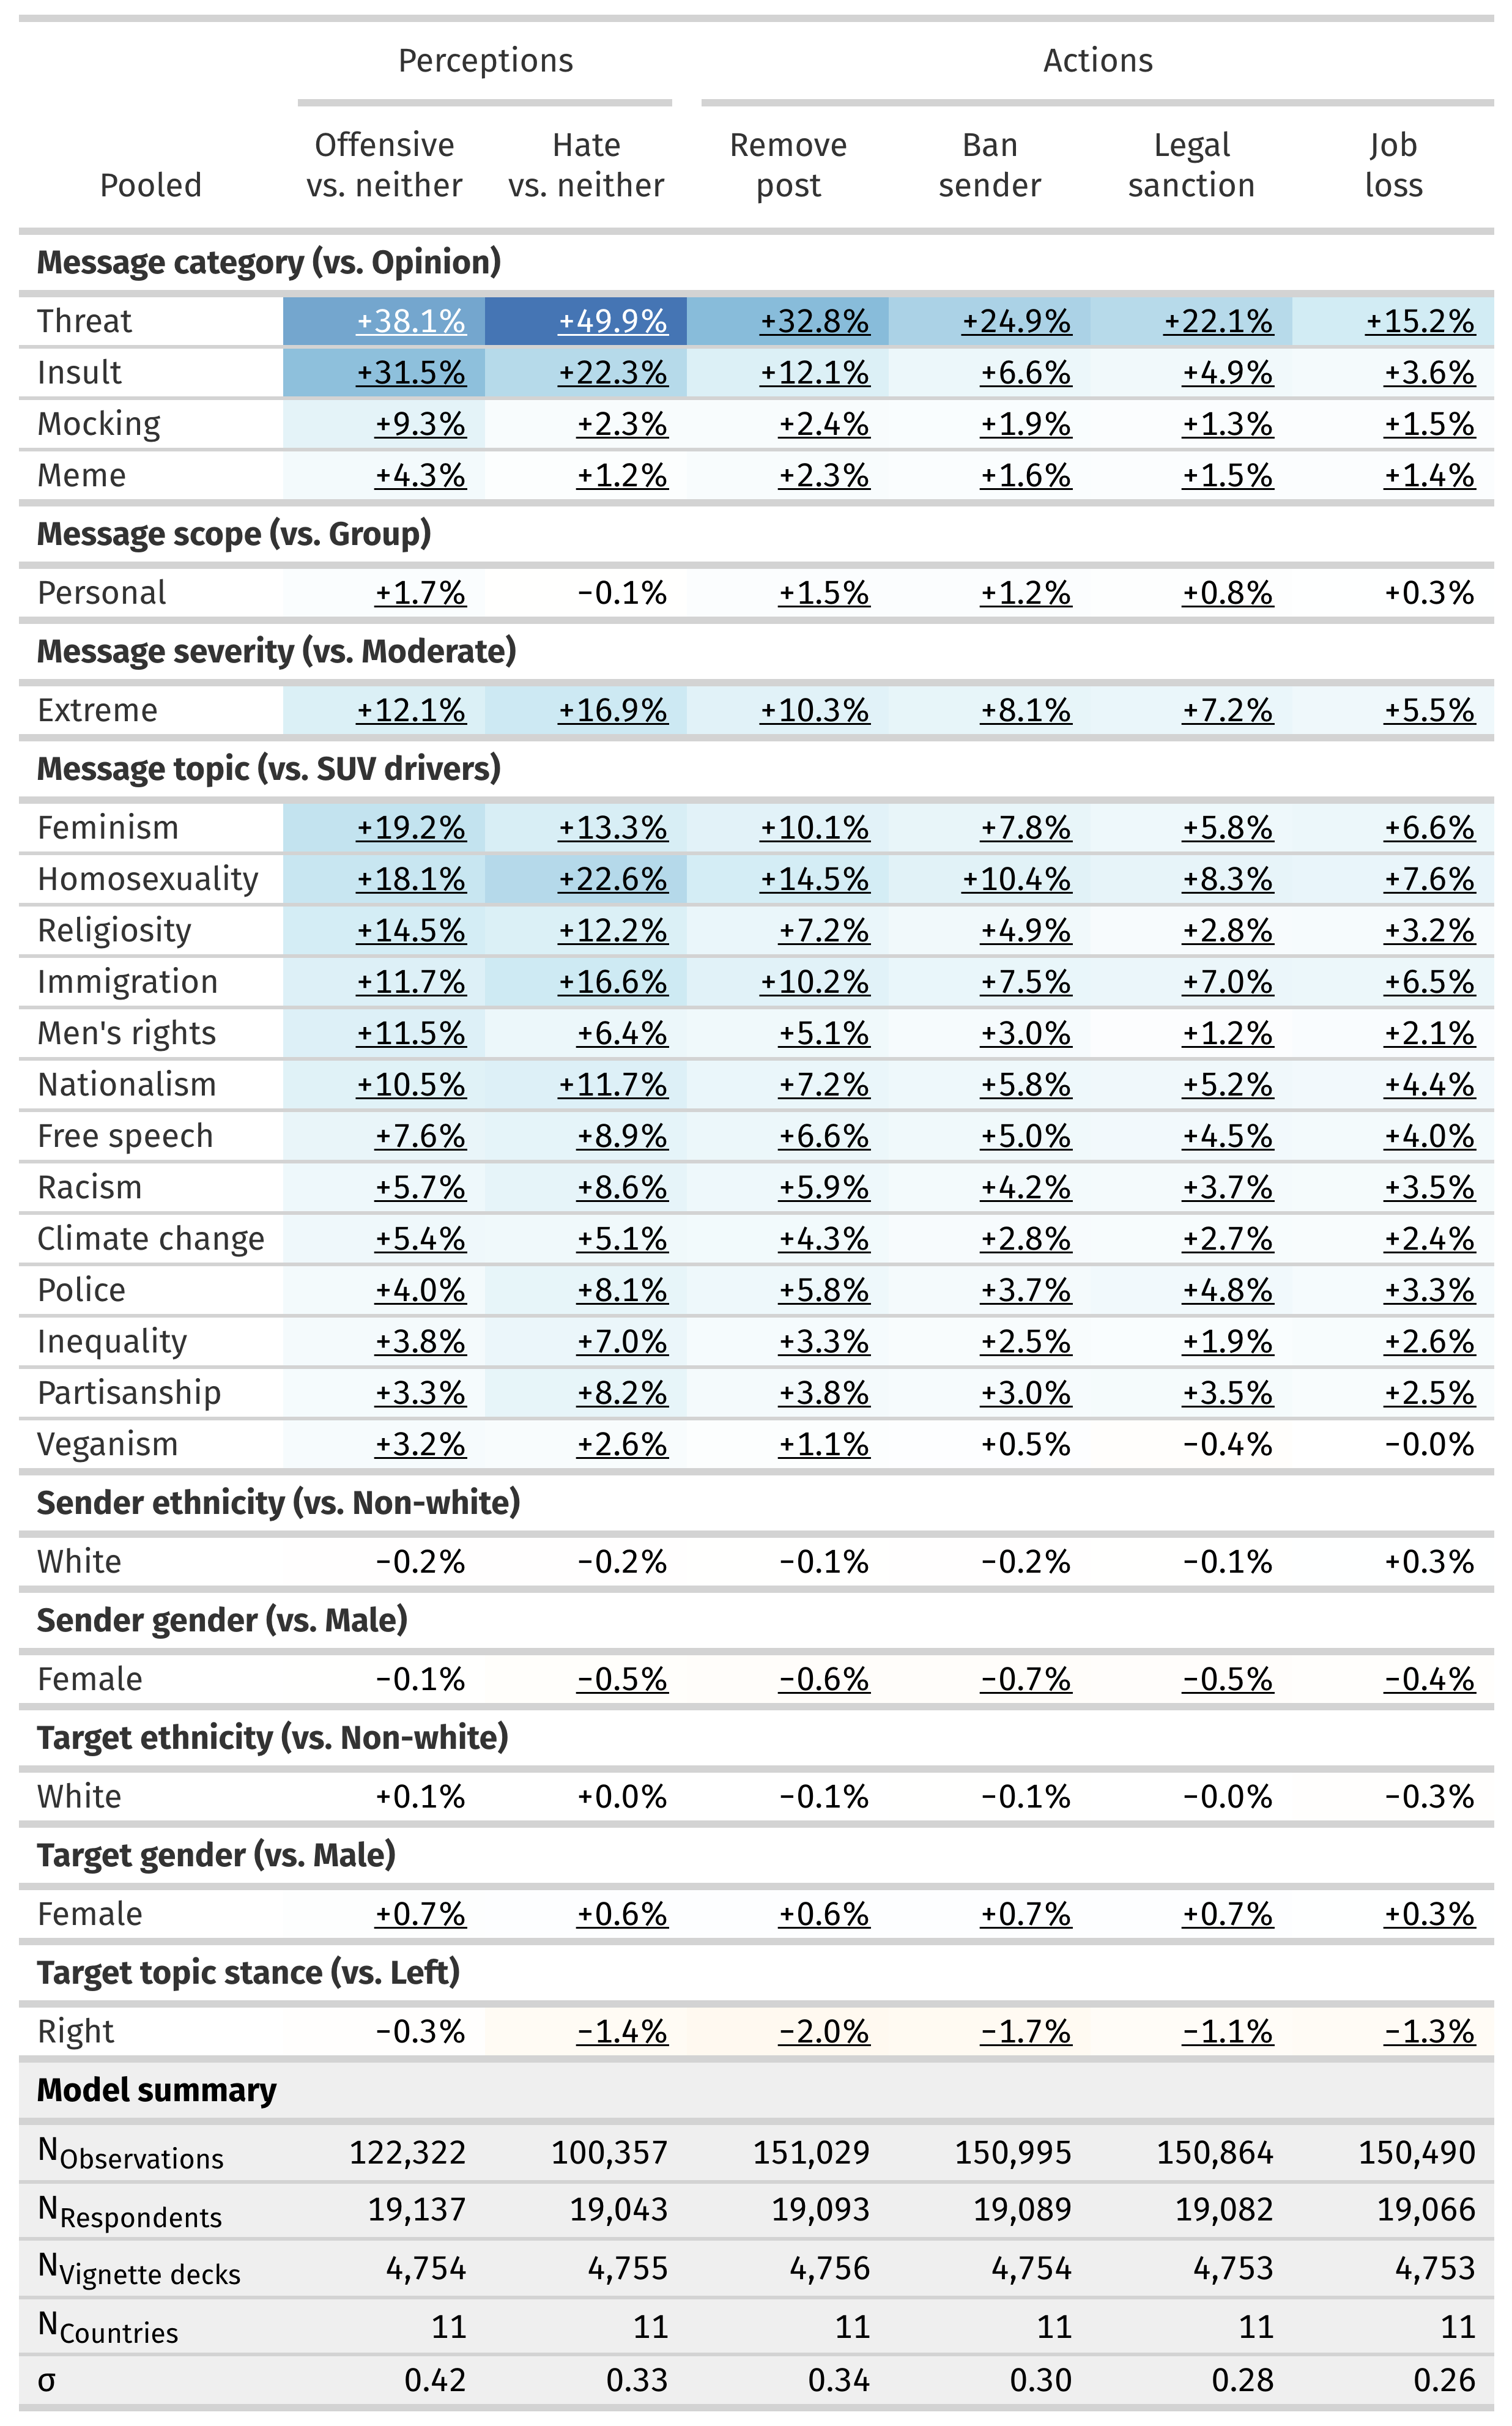
\includegraphics[width=.7\linewidth]{figures/table-acme-pooled.png}
\caption{\textbf{Average marginal component effects (AMCEs) of social media post characteristics on people's perceptions and preferred sanctions.\\} Estimated from hierarchical linear models with respondent, vignette deck, and country random effects. All outcomes are binary; Reported estimates represent percentage-point differences in choice probabilities compared to the respective baseline category. Underlined estimates are significantly different from 0 with $p<0.05$. The color shading highlights the effect sizes.}
\label{fig:table-acme-pooled}
\end{figure*}

\begin{figure*}[t!]
  \centering
\includegraphics[width=.7\linewidth]{figures/table-mm-pooled.png}
\caption{\textbf{Estimated marginal means of social media post characteristics on people's perceptions and preferred sanctions.\\} Estimated from hierarchical linear models with respondent, vignette deck, and country random effects. All outcomes are binary; reported estimates represent predicted choice probabilities for each category. The color shading highlights the marginal means.}
\label{fig:table-mm-pooled}
\end{figure*}

\begin{figure*}[t!]
  \centering
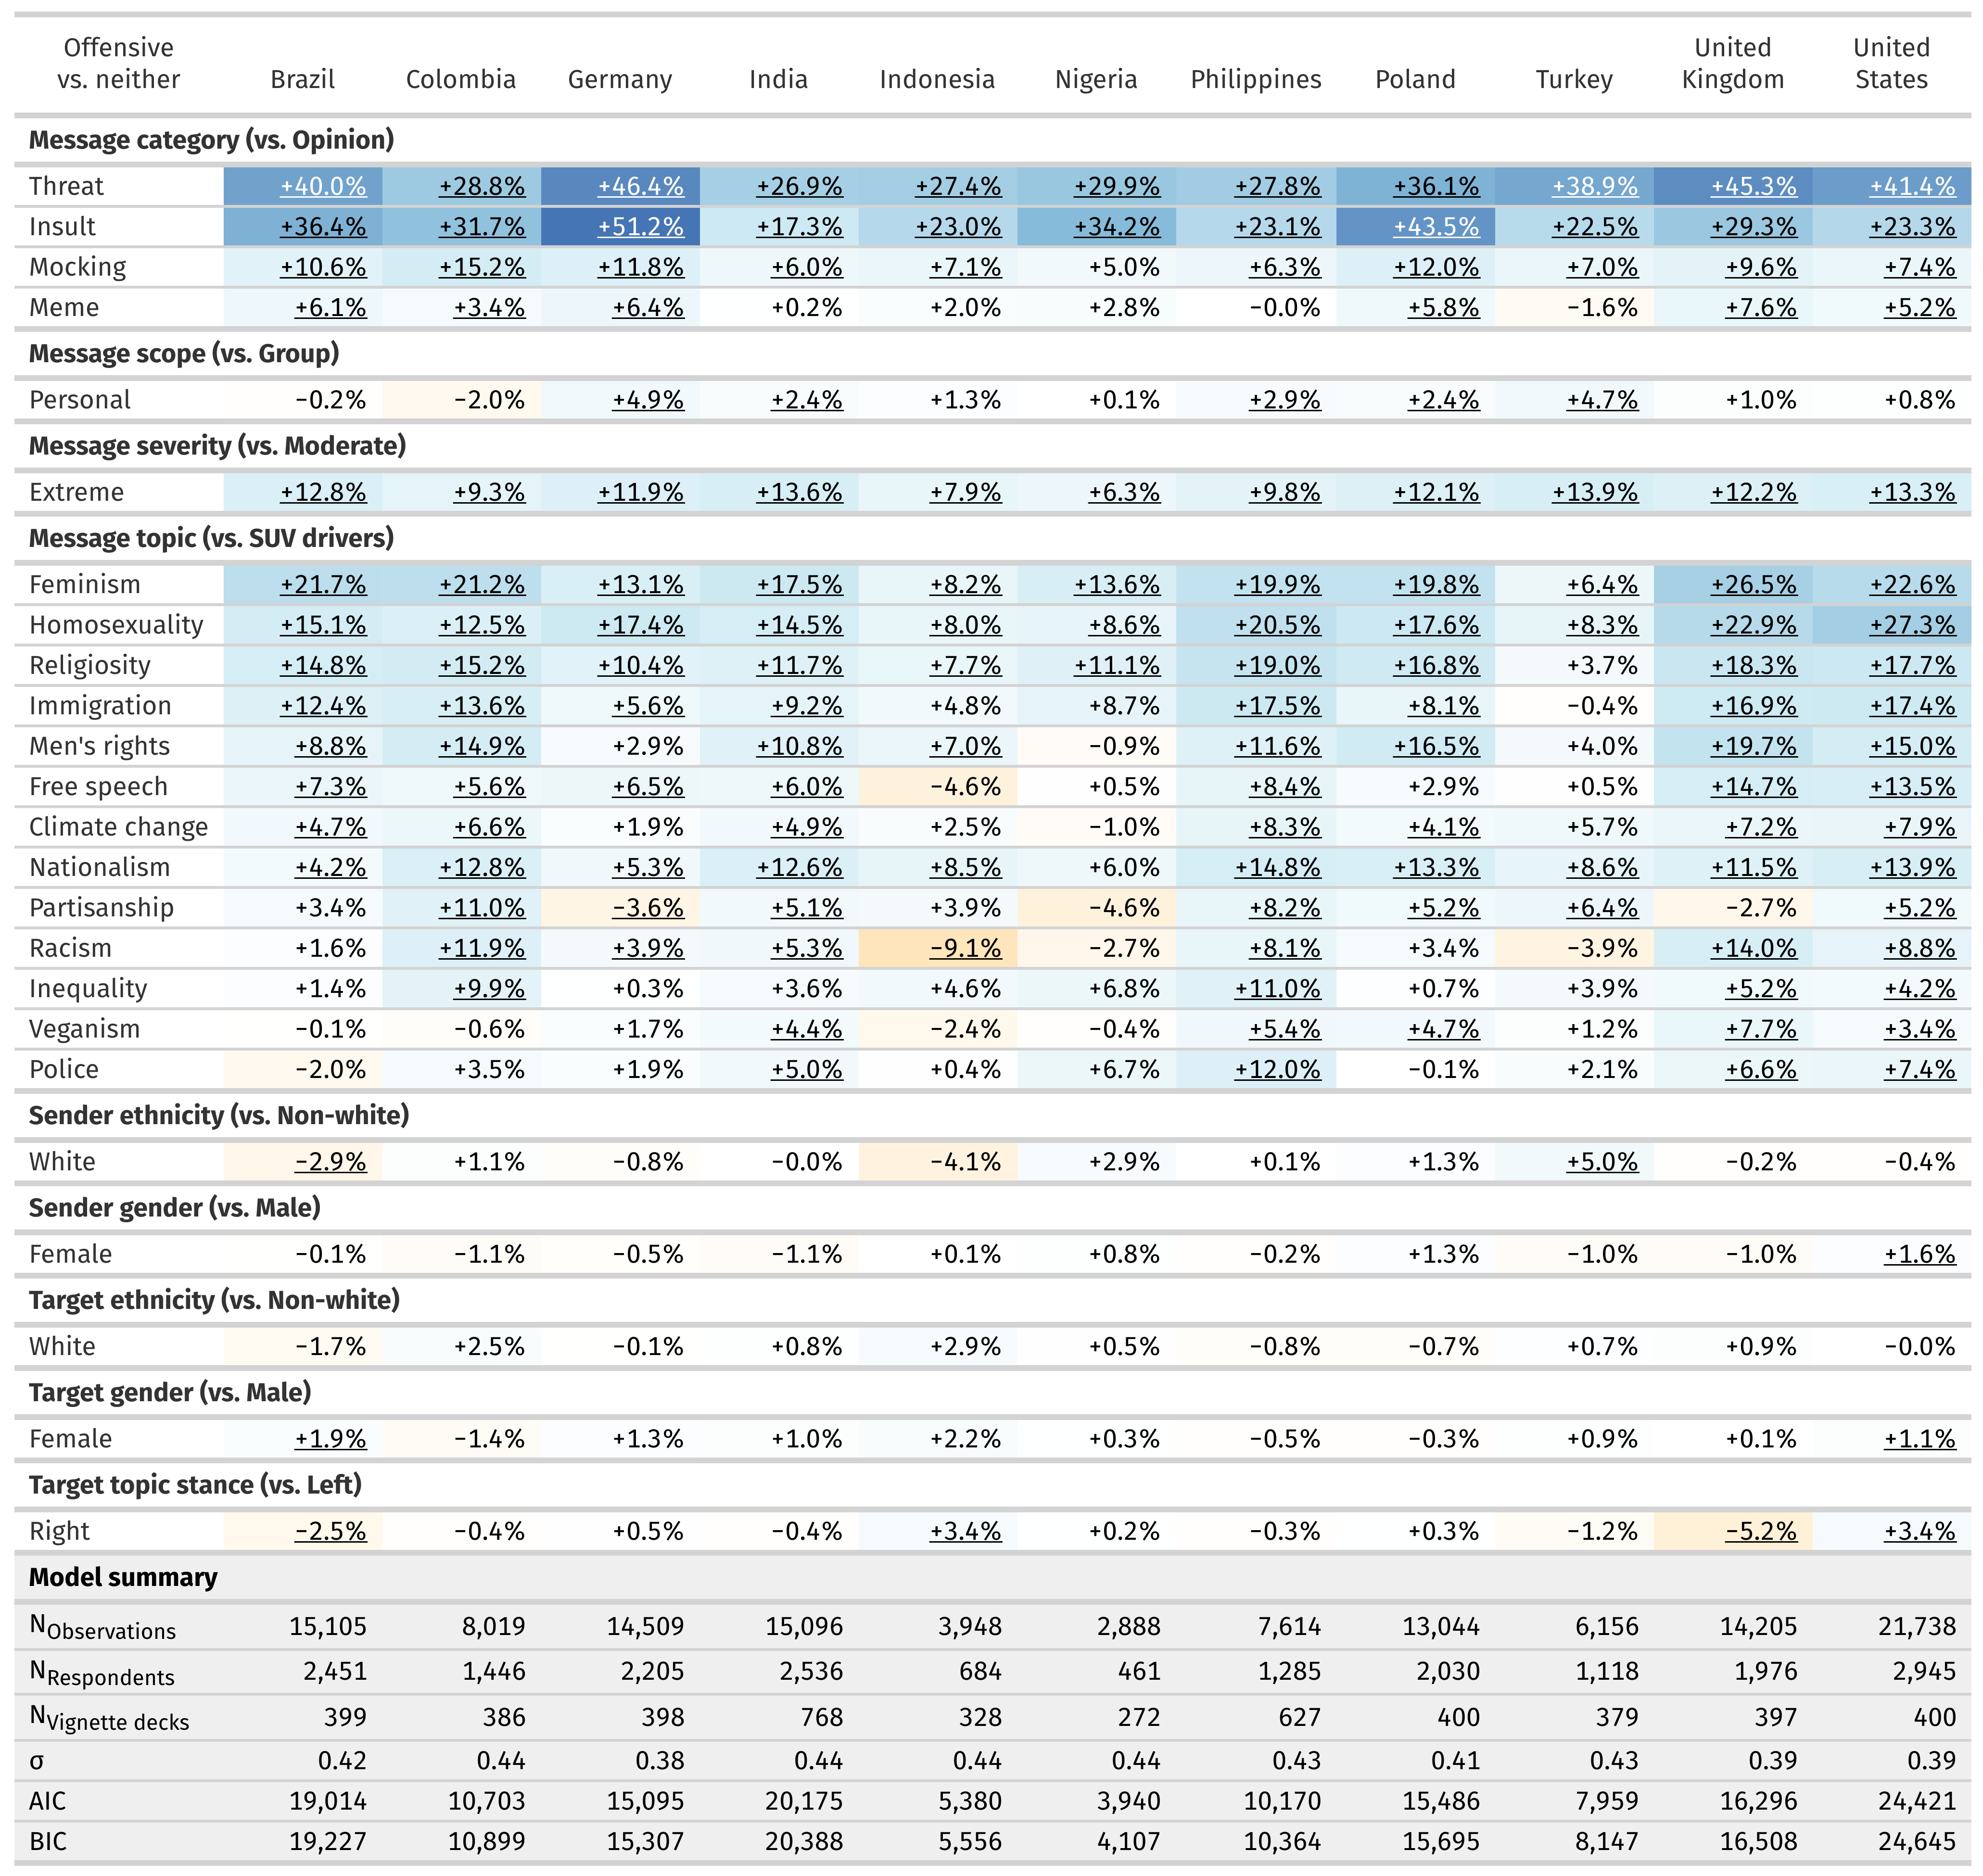
\includegraphics[width=1\linewidth]{figures/table-acme-vig_perc_offensive2.png}
\caption{\textbf{AMCEs of social media post characteristics on \uline{perceived offensiveness}, by country.\\} Estimated from hierarchical linear models with respondent and vignette deck effects. Reported estimates represent percentage-point differences in choice probabilities. Underlined estimates are significantly different from 0 with $p<0.05$. The color shading highlights the effect sizes.}
\label{fig:table-acme-vig_perc_offensive2}
\end{figure*}

\begin{figure*}[t!]
  \centering
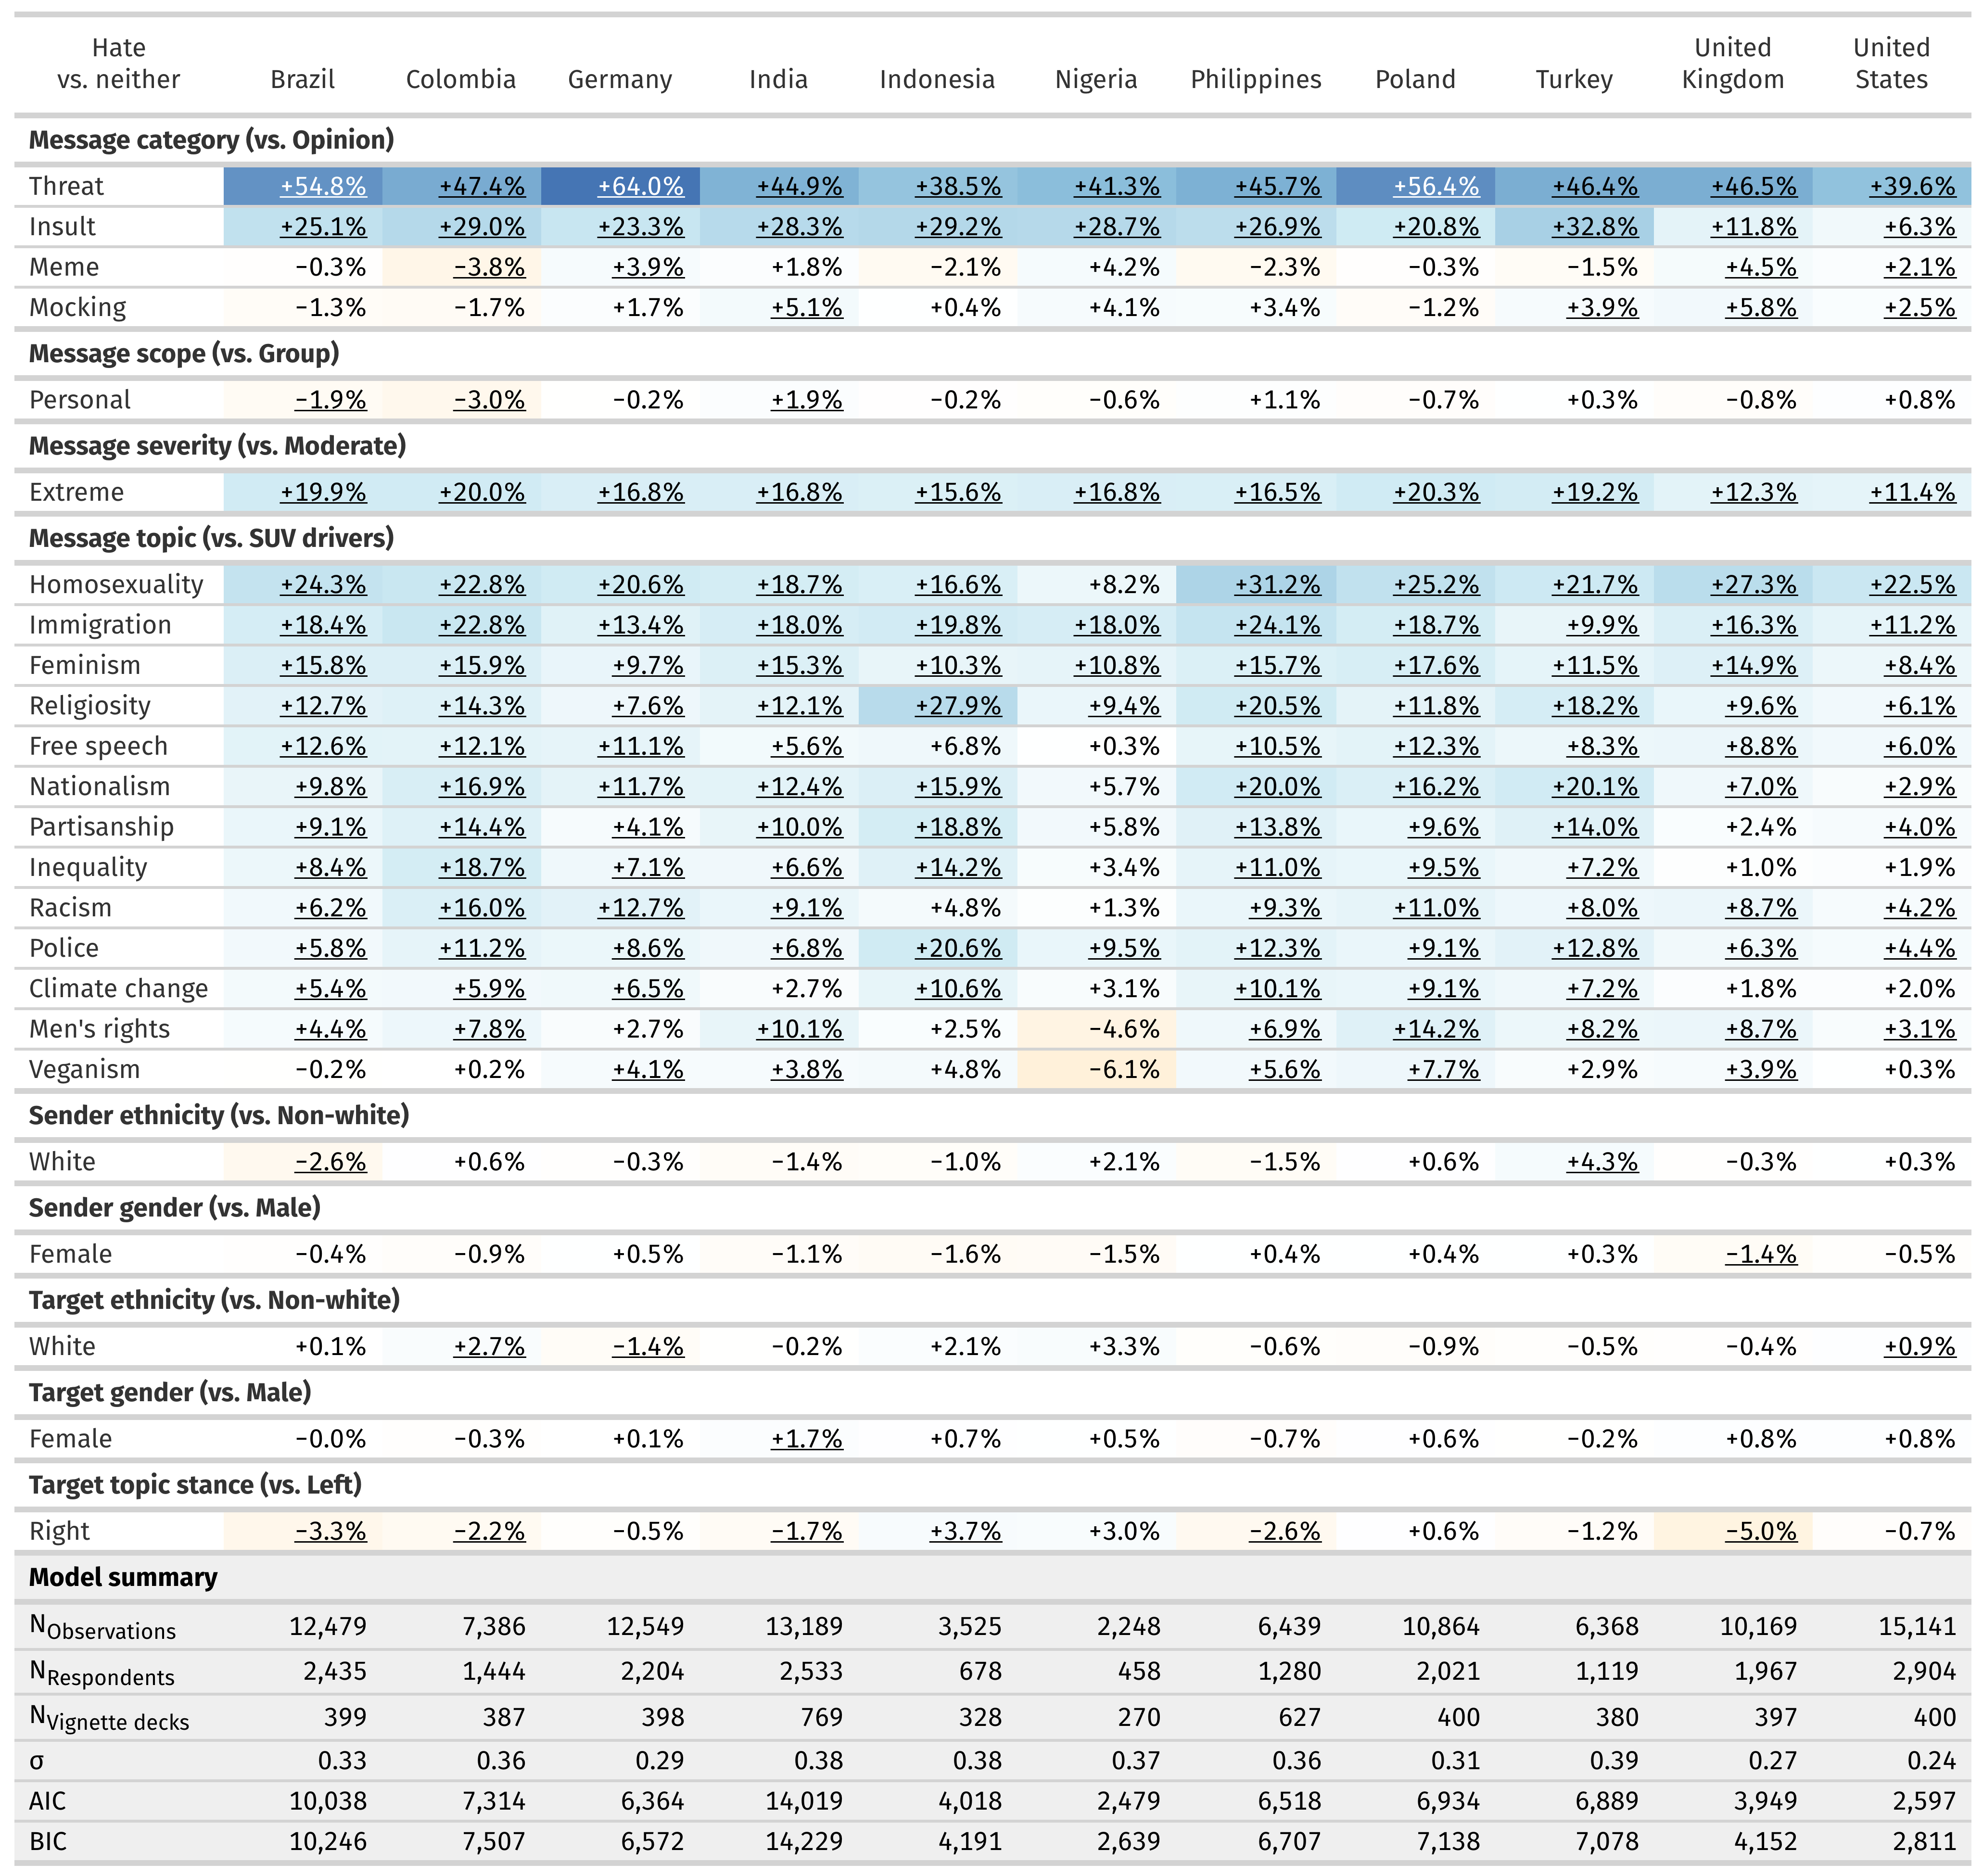
\includegraphics[width=1\linewidth]{figures/table-acme-vig_perc_hate2.png}
\caption{\textbf{AMCEs of social media post characteristics on \uline{perceived hate speech}, by country.\\} Estimated from hierarchical linear models with respondent and vignette deck effects. Reported estimates represent percentage-point differences in choice probabilities. Underlined estimates are significantly different from 0 with $p<0.05$. The color shading highlights the effect sizes.}
\label{fig:table-acme-vig_perc_hate2}
\end{figure*}

\begin{figure*}[t!]
  \centering
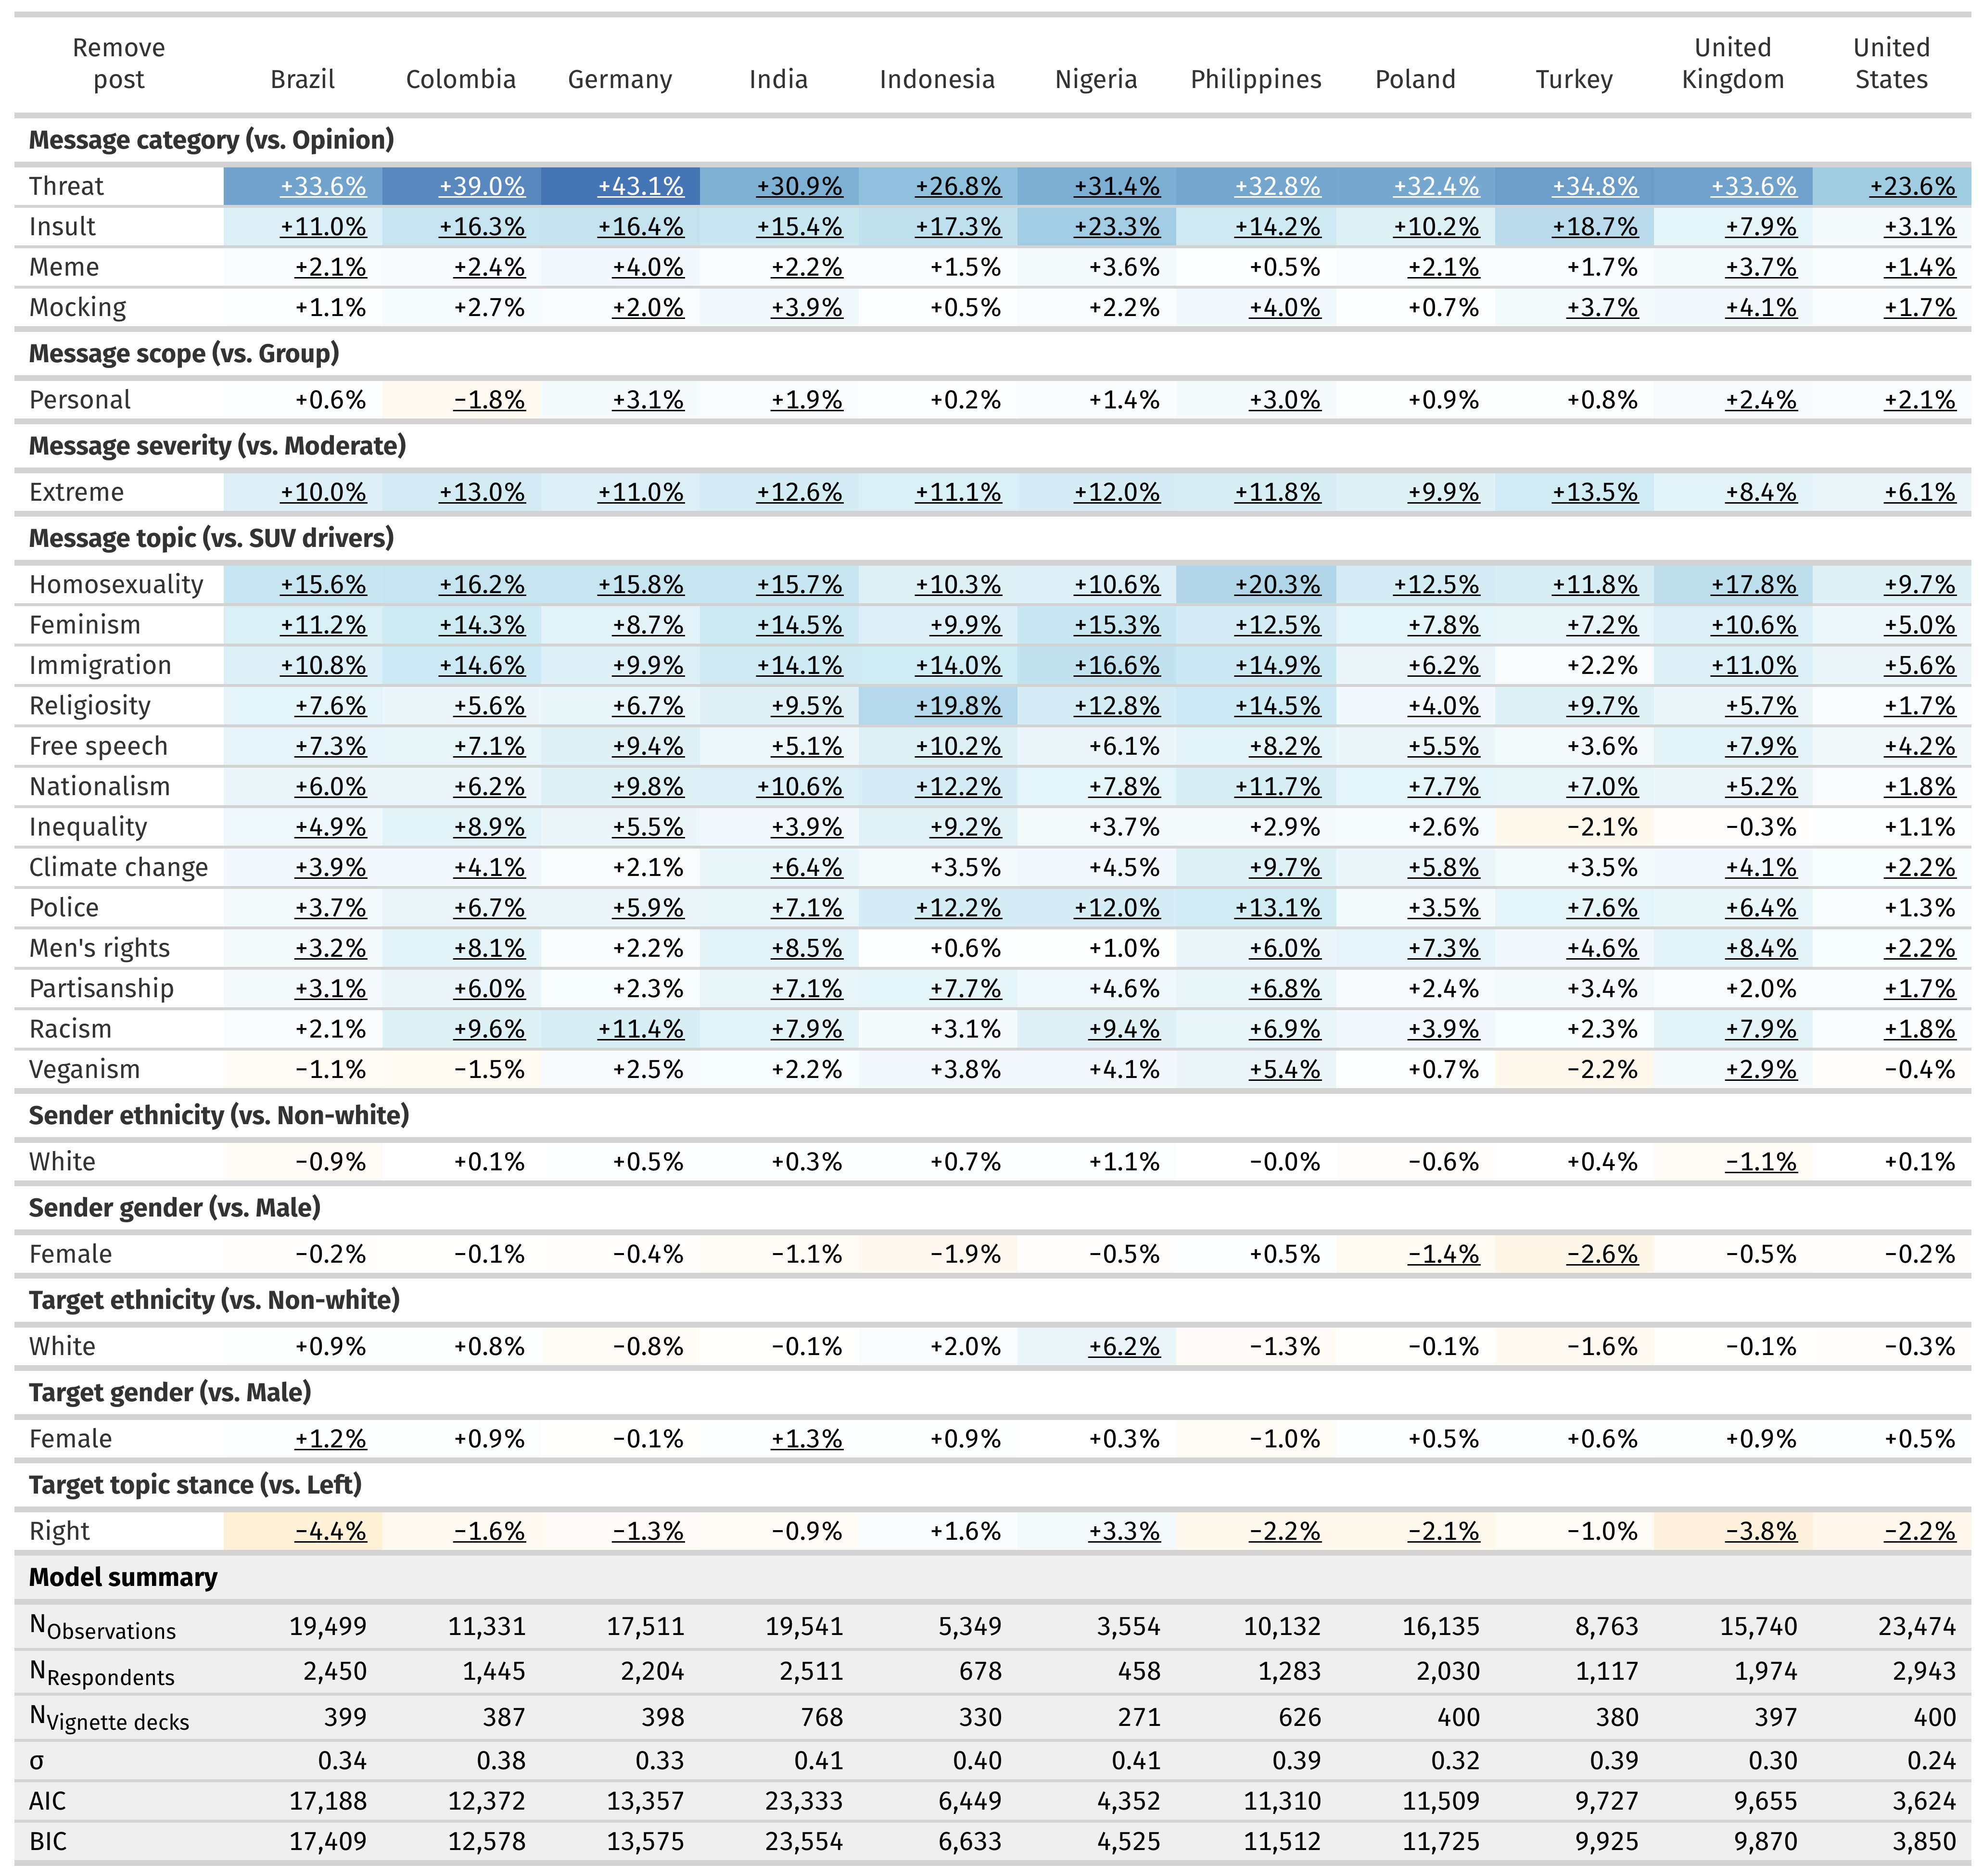
\includegraphics[width=1\linewidth]{figures/table-acme-vig_remove.png}
\caption{\textbf{AMCEs of social media post characteristics on \uline{preference for removal}, by country.\\} Estimated from hierarchical linear models with respondent and vignette deck effects. Reported estimates represent percentage-point differences in choice probabilities. Underlined estimates are significantly different from 0 with $p<0.05$. The color shading highlights the effect sizes.}
\label{fig:table-acme-vig_perc_remove}
\end{figure*}

\begin{figure*}[t!]
  \centering
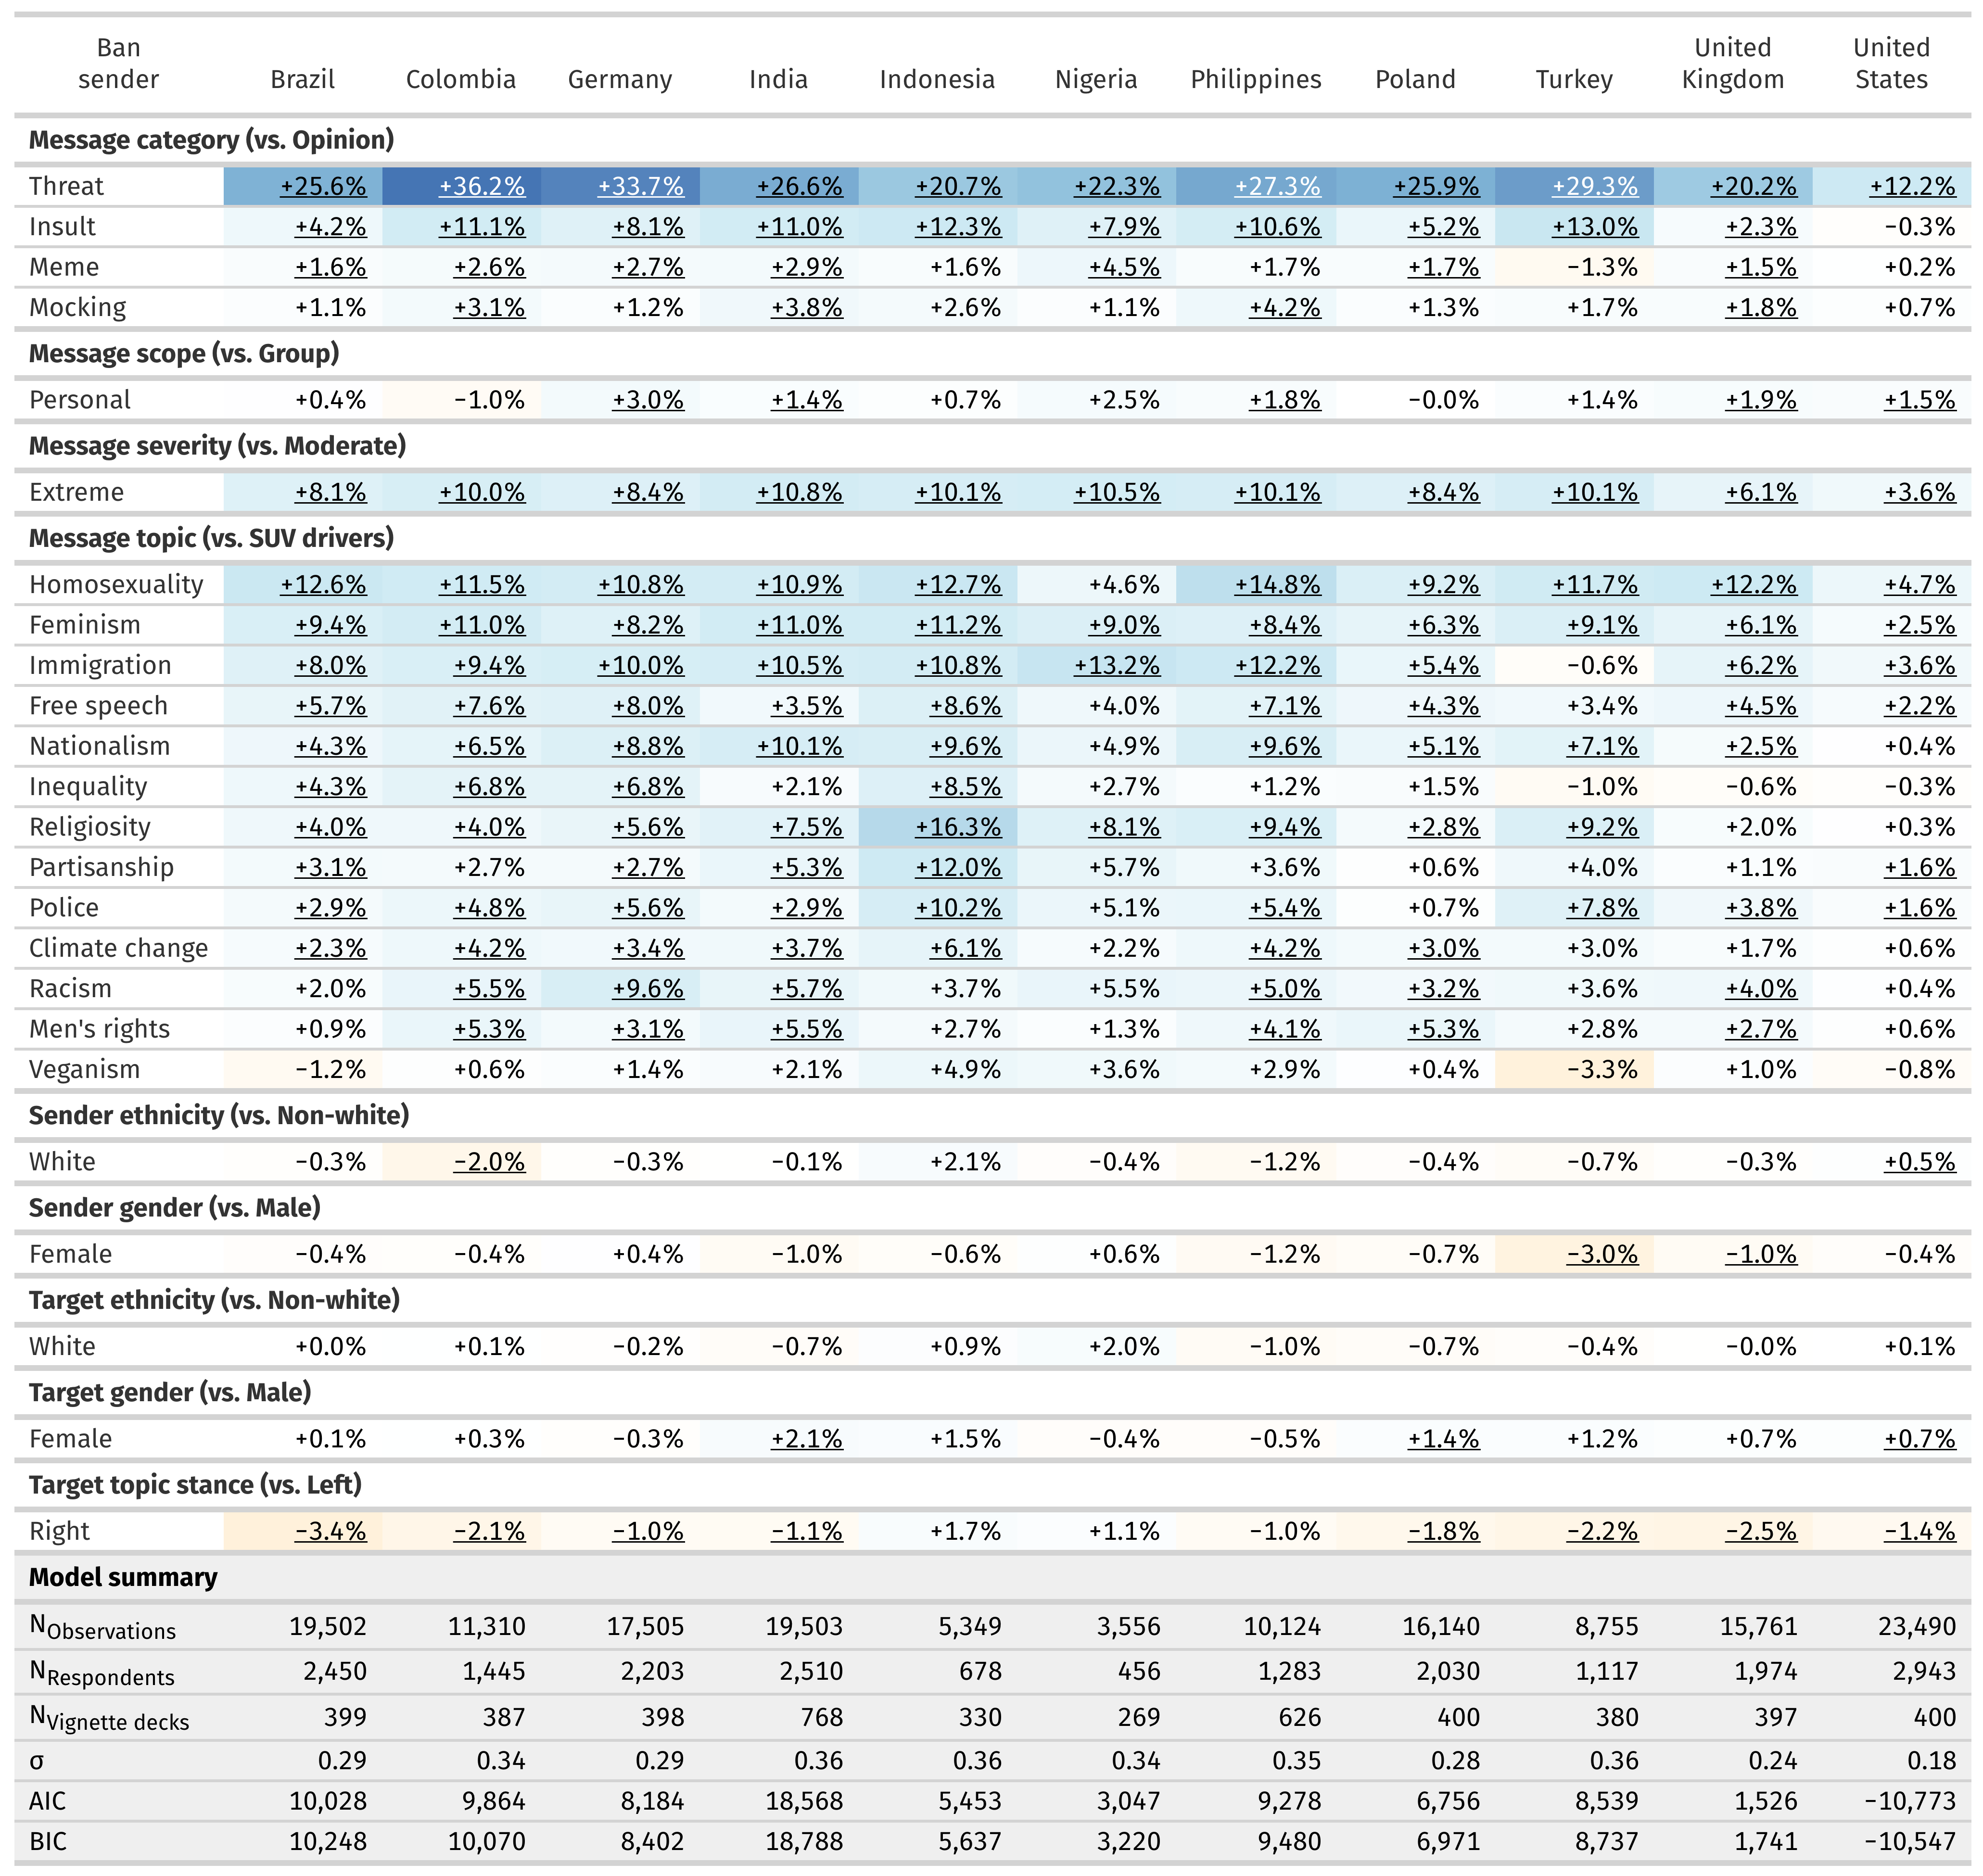
\includegraphics[width=1\linewidth]{figures/table-acme-vig_ban.png}
\caption{\textbf{AMCEs of social media post characteristics on \uline{preference for user ban}, by country.\\} Estimated from hierarchical linear models with respondent and vignette deck effects. Reported estimates represent percentage-point differences in choice probabilities. Underlined estimates are significantly different from 0 with $p<0.05$. The color shading highlights the effect sizes.}
\label{fig:table-acme-vig_perc_ban}
\end{figure*}

\begin{figure*}[t!]
  \centering
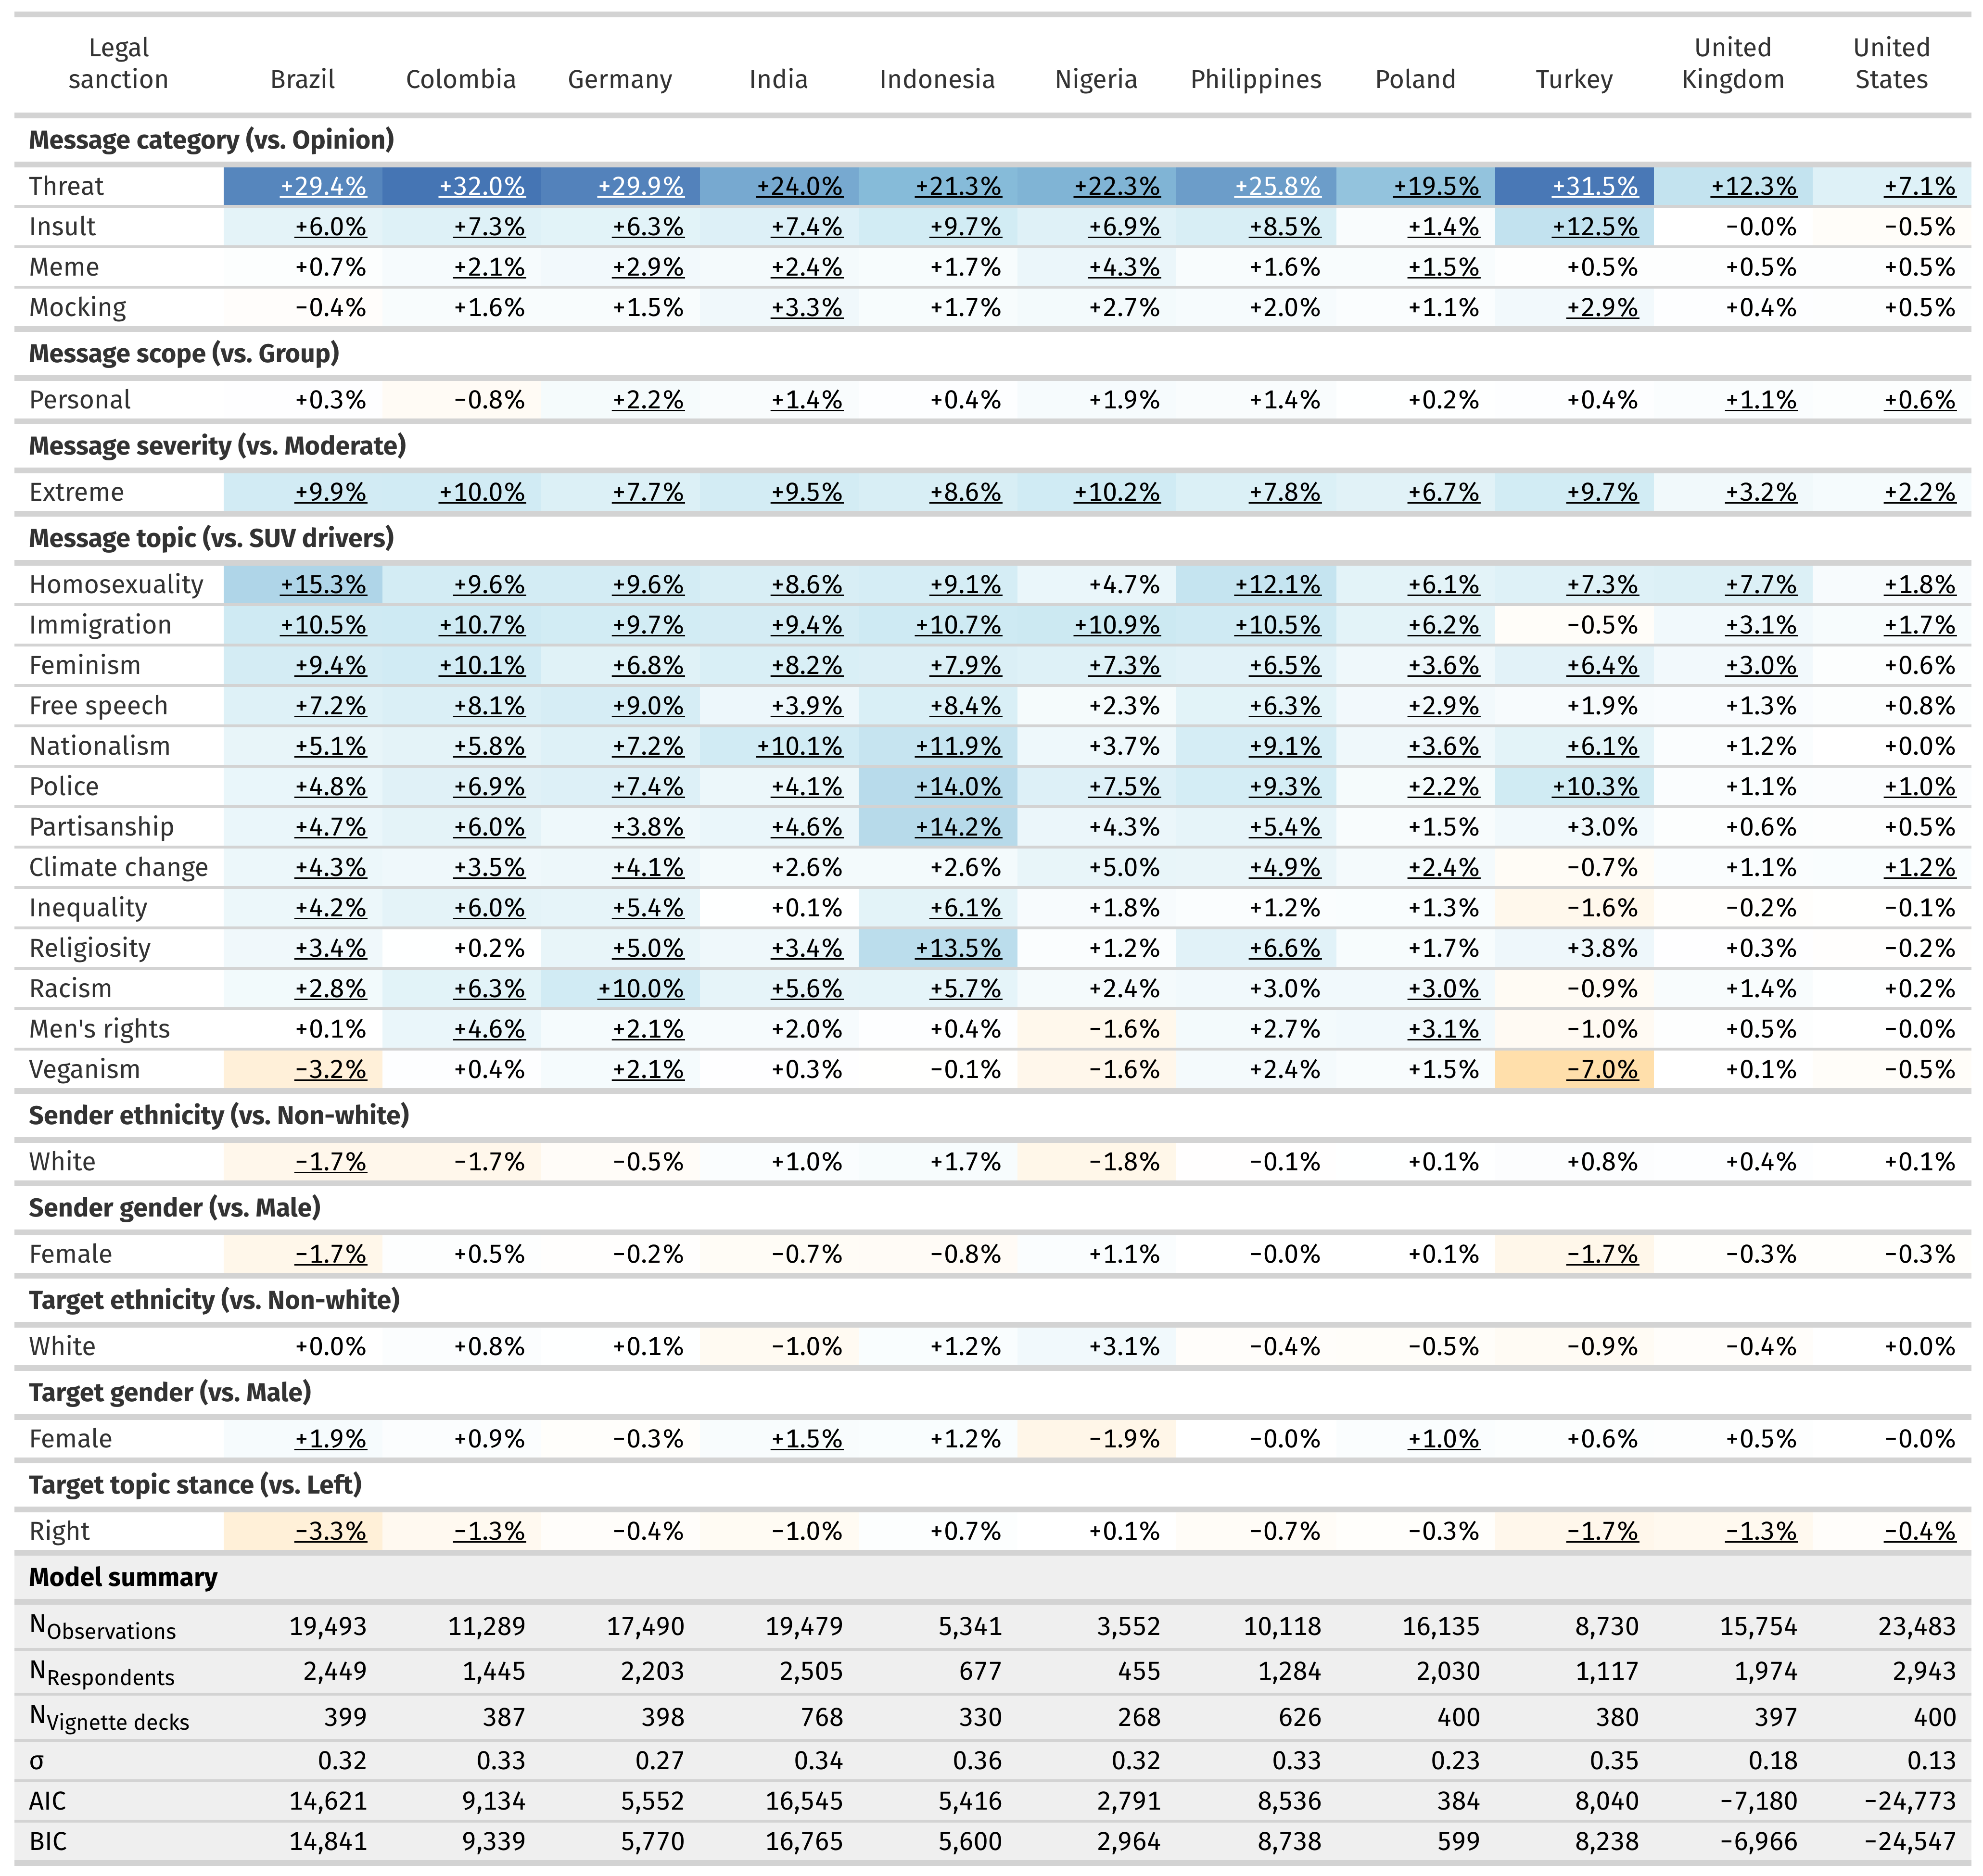
\includegraphics[width=1\linewidth]{figures/table-acme-vig_legal.png}
\caption{\textbf{AMCEs of social media post characteristics on \uline{preference for legal consequences for user}, by country.\\} Estimated from hierarchical linear models with respondent and vignette deck effects. Reported estimates represent percentage-point differences in choice probabilities. Underlined estimates are significantly different from 0 with $p<0.05$. The color shading highlights the effect sizes.}
\label{fig:table-acme-vig_perc_legal}
\end{figure*}

\begin{figure*}[t!]
  \centering
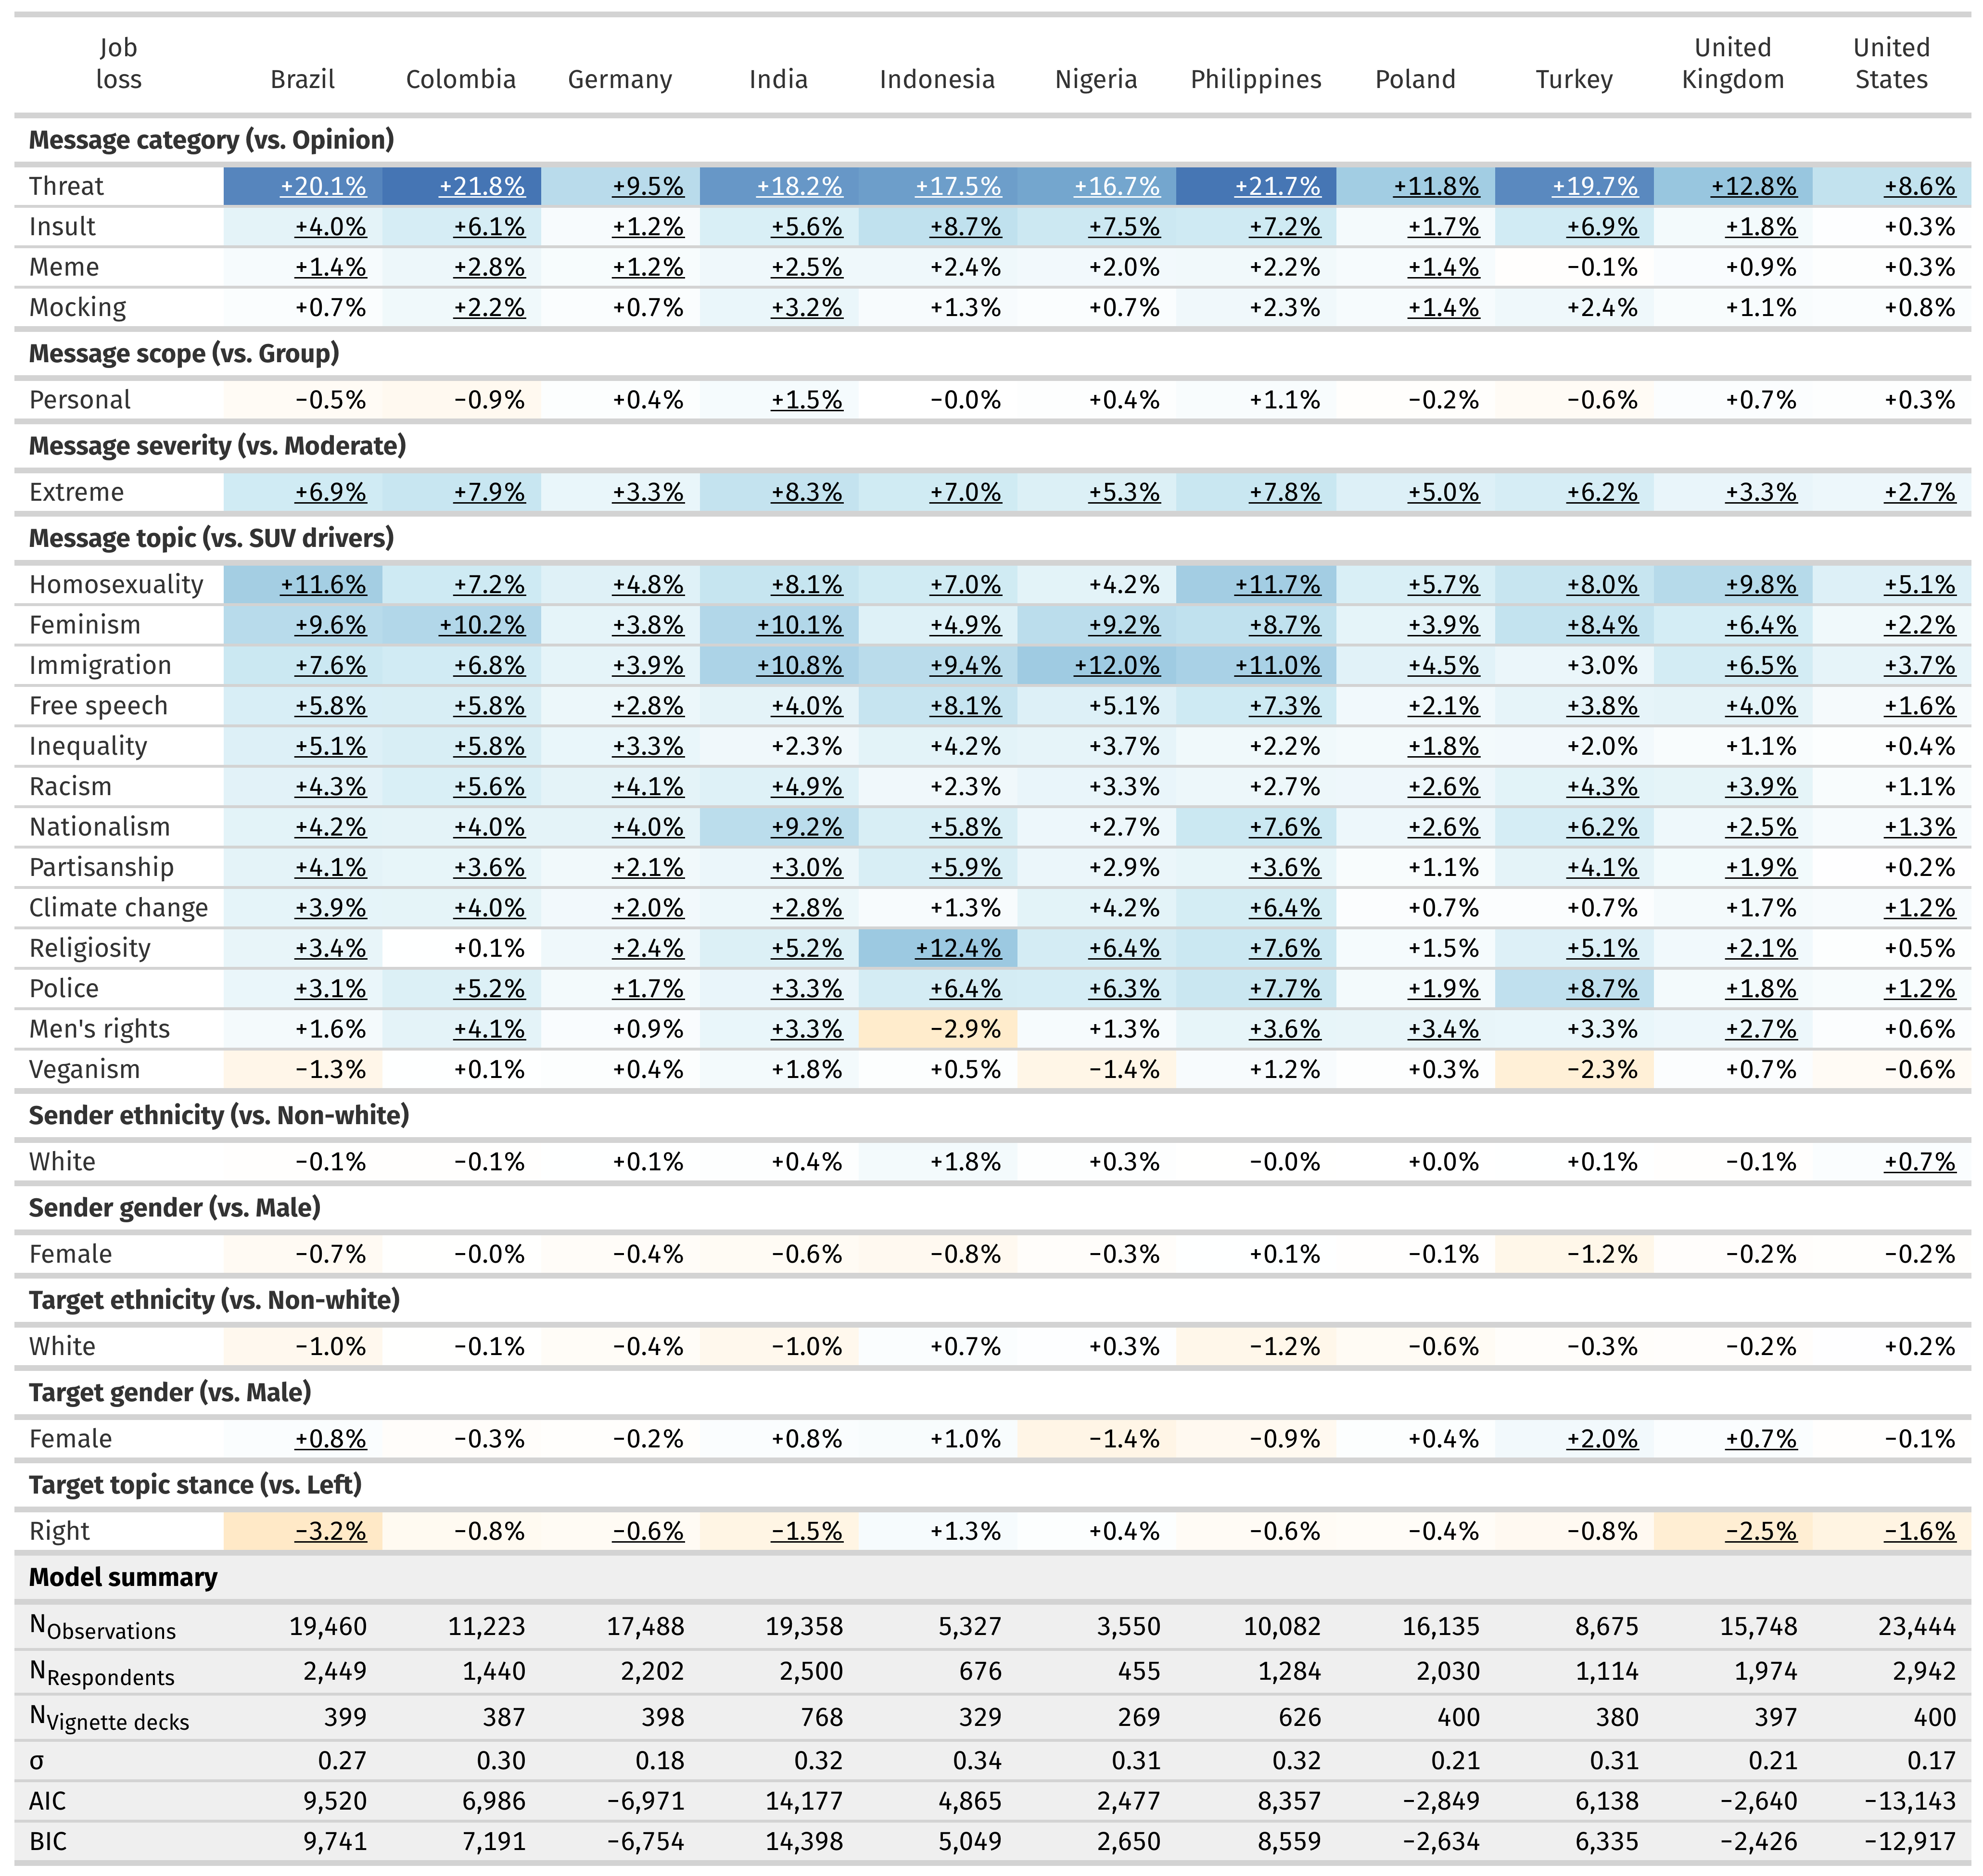
\includegraphics[width=1\linewidth]{figures/table-acme-vig_job.png}
\caption{\textbf{AMCEs of social media post characteristics on \uline{preference for job loss of user}, by country.\\} Estimated from hierarchical linear models with respondent and vignette deck effects. Reported estimates represent percentage-point differences in choice probabilities. Underlined estimates are significantly different from 0 with $p<0.05$. The color shading highlights the effect sizes.}
\label{fig:table-acme-vig_perc_job}
\end{figure*}

\begin{figure*}[t!]
  \centering
    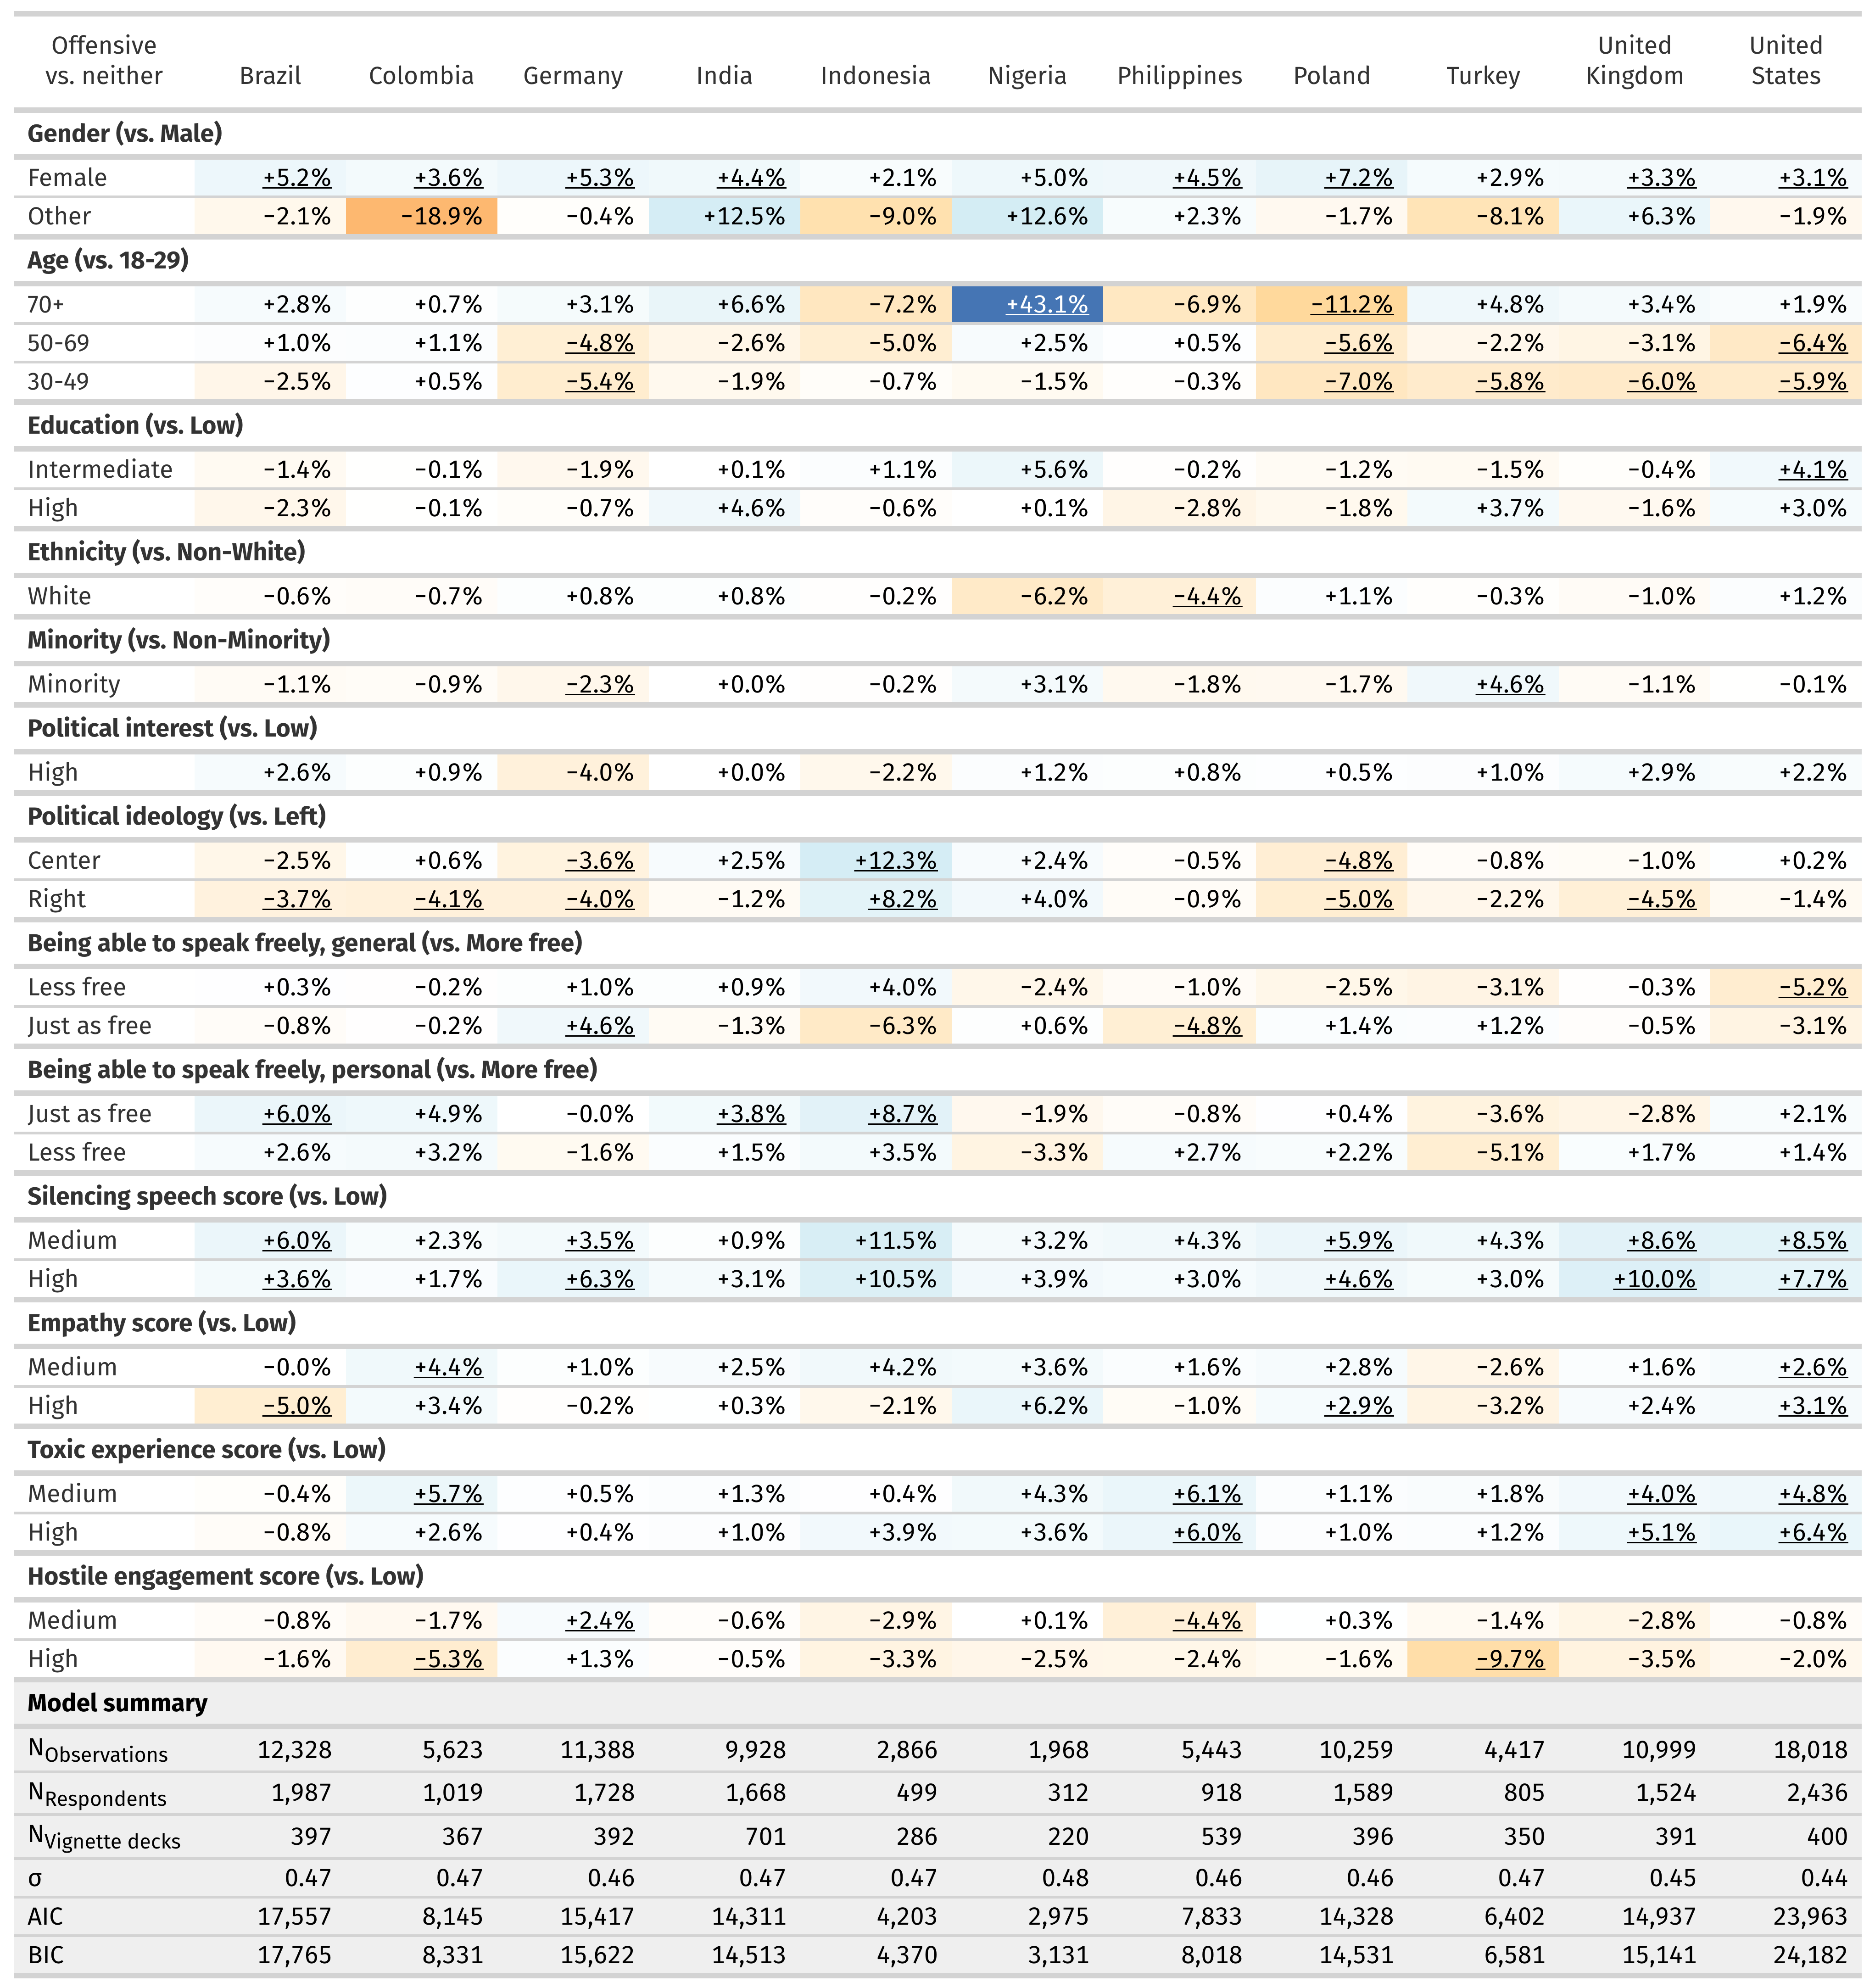
\includegraphics[width=1\linewidth]{figures/table-respmodels-vig_perc_offensive2.png}
\caption{\textbf{Effects of respondent characteristics on \uline{perceived offensiveness}, by country.\\} Estimated from hierarchical linear models with respondent and vignette deck effects. Reported estimates represent percentage-point differences in choice probabilities. Underlined estimates are significantly different from 0 with $p<0.05$. The color shading highlights the effect sizes.}
\label{fig:table-respmodels-vig_perc_offensive2}
\end{figure*}

\begin{figure*}[t!]
  \centering
    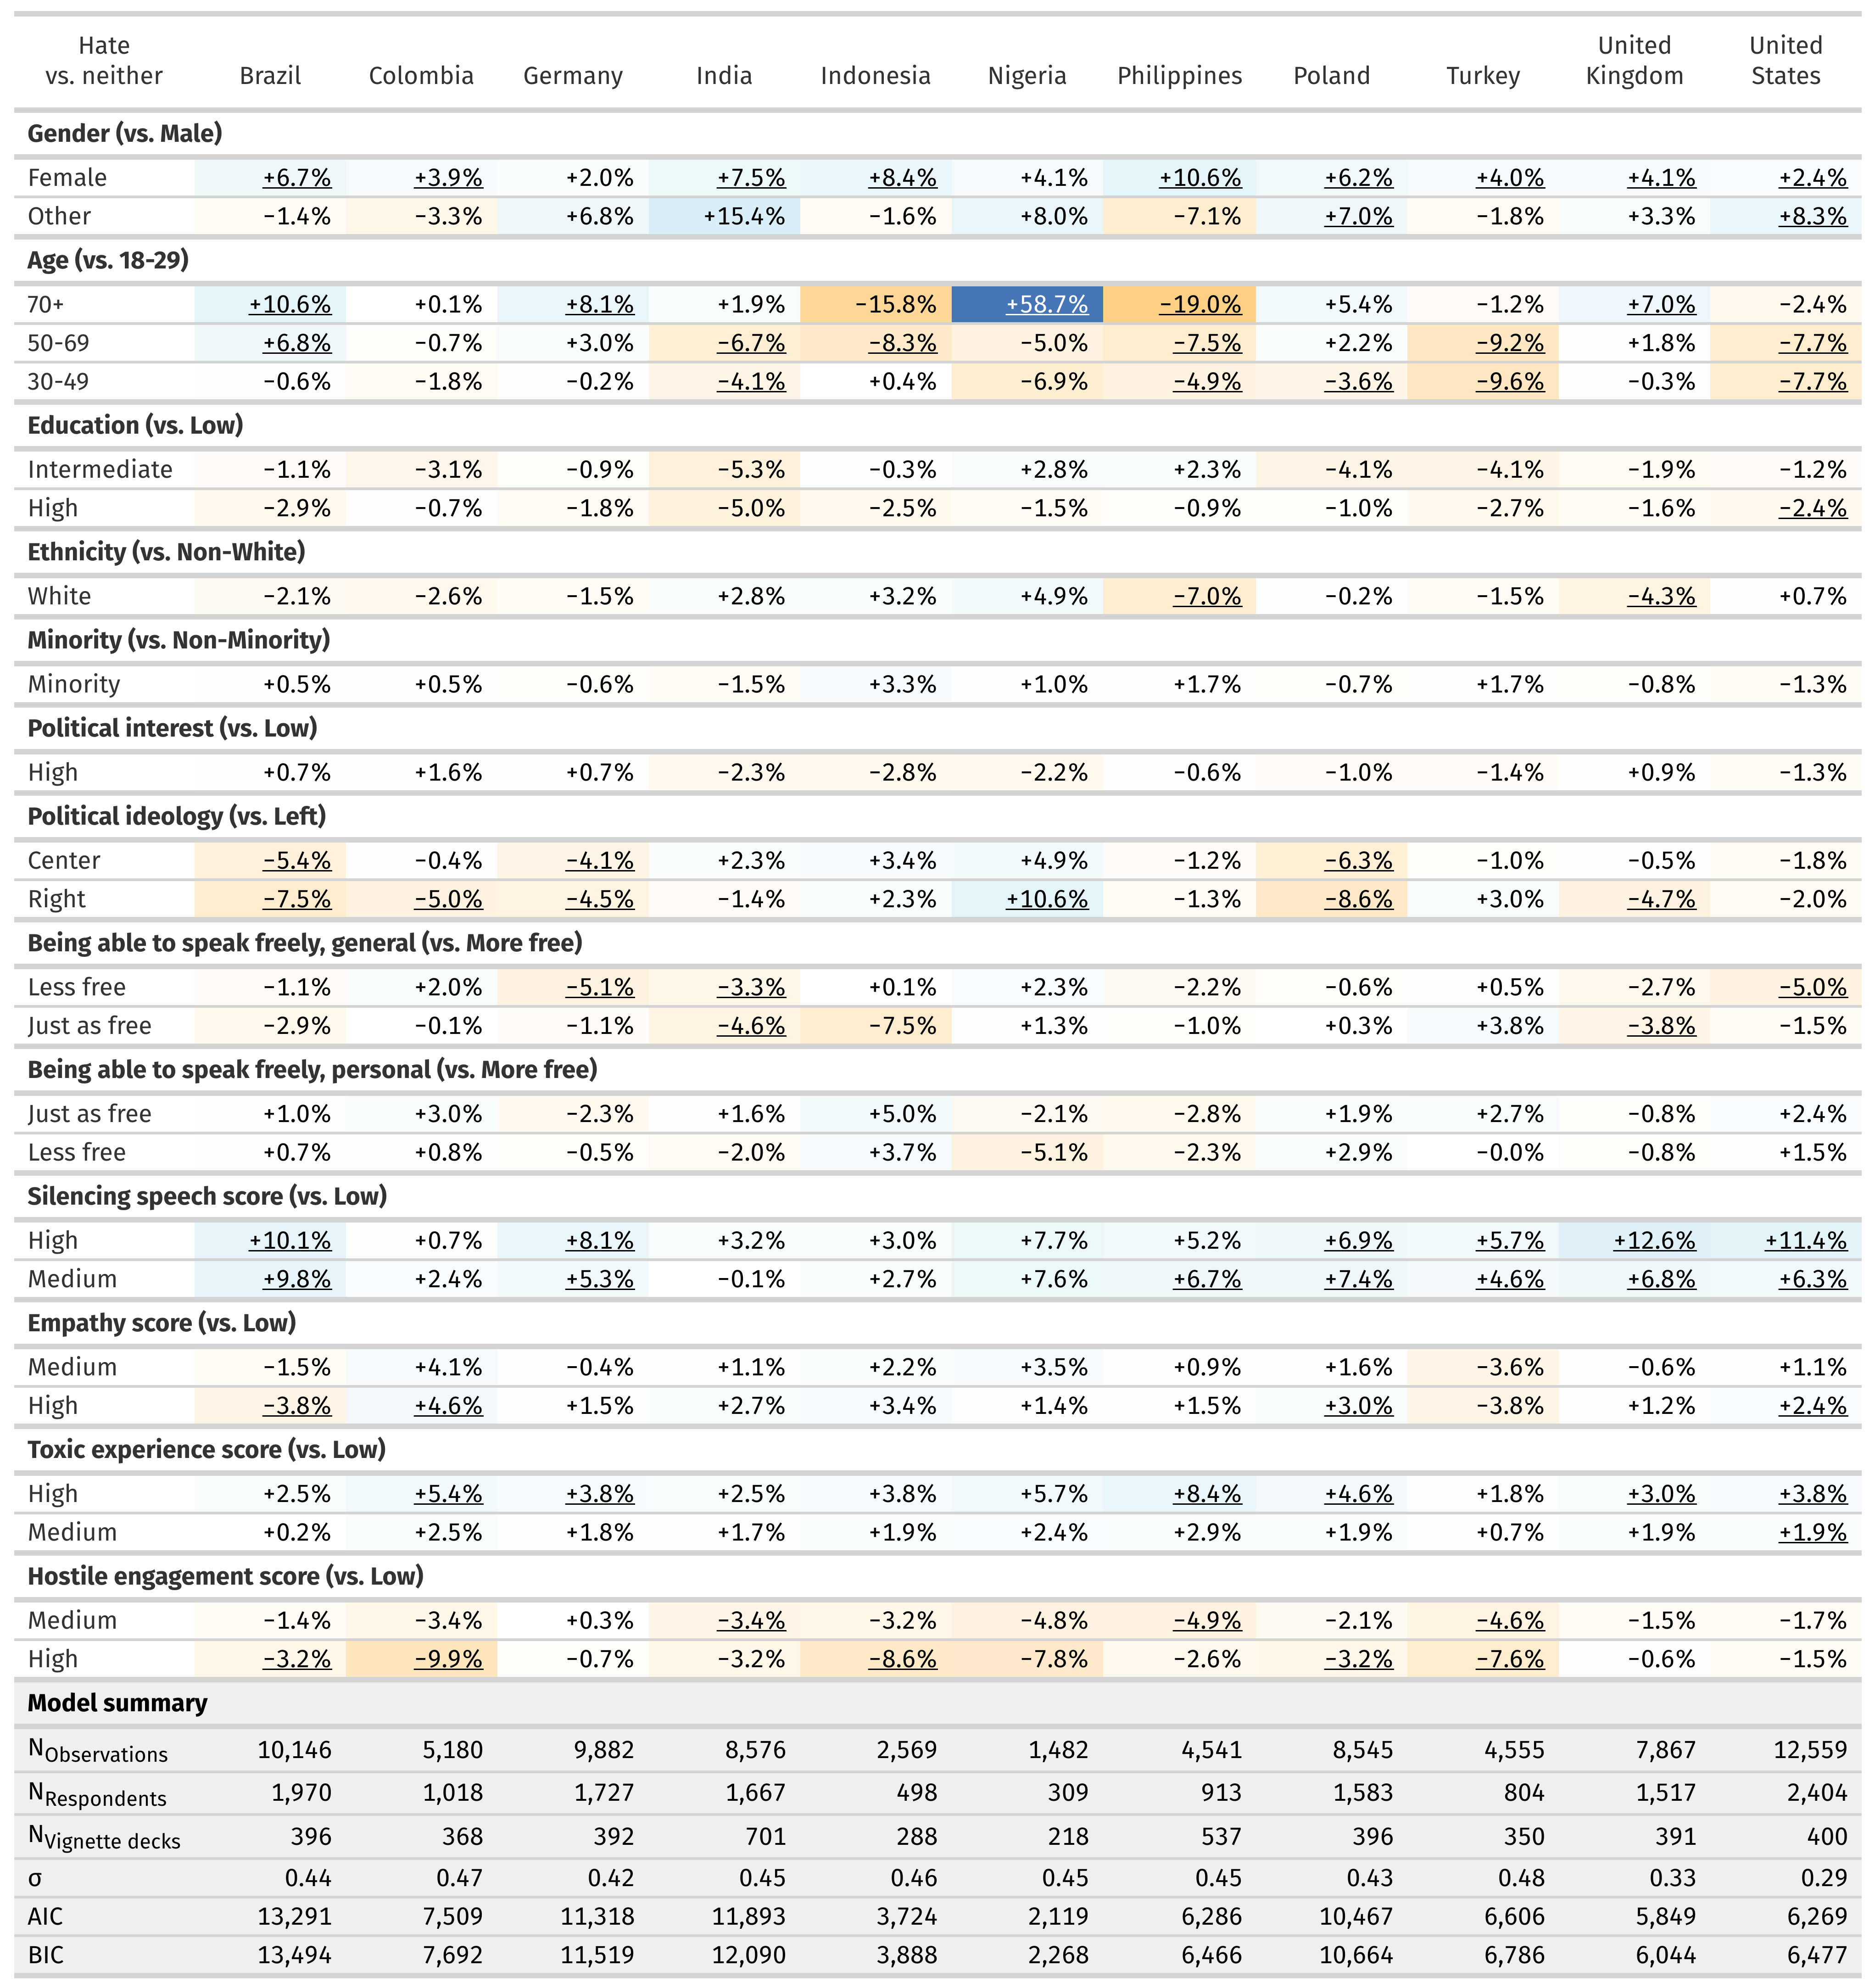
\includegraphics[width=1\linewidth]{figures/table-respmodels-vig_perc_hate2.png}
\caption{\textbf{Effects of respondent characteristics on \uline{perceived hate speech}, by country.\\} Estimated from hierarchical linear models with respondent and vignette deck effects. Reported estimates represent percentage-point differences in choice probabilities. Underlined estimates are significantly different from 0 with $p<0.05$. The color shading highlights the effect sizes.}
\label{fig:table-respmodels-vig_perc_hate2}
\end{figure*}

\begin{figure*}[t!]
  \centering
    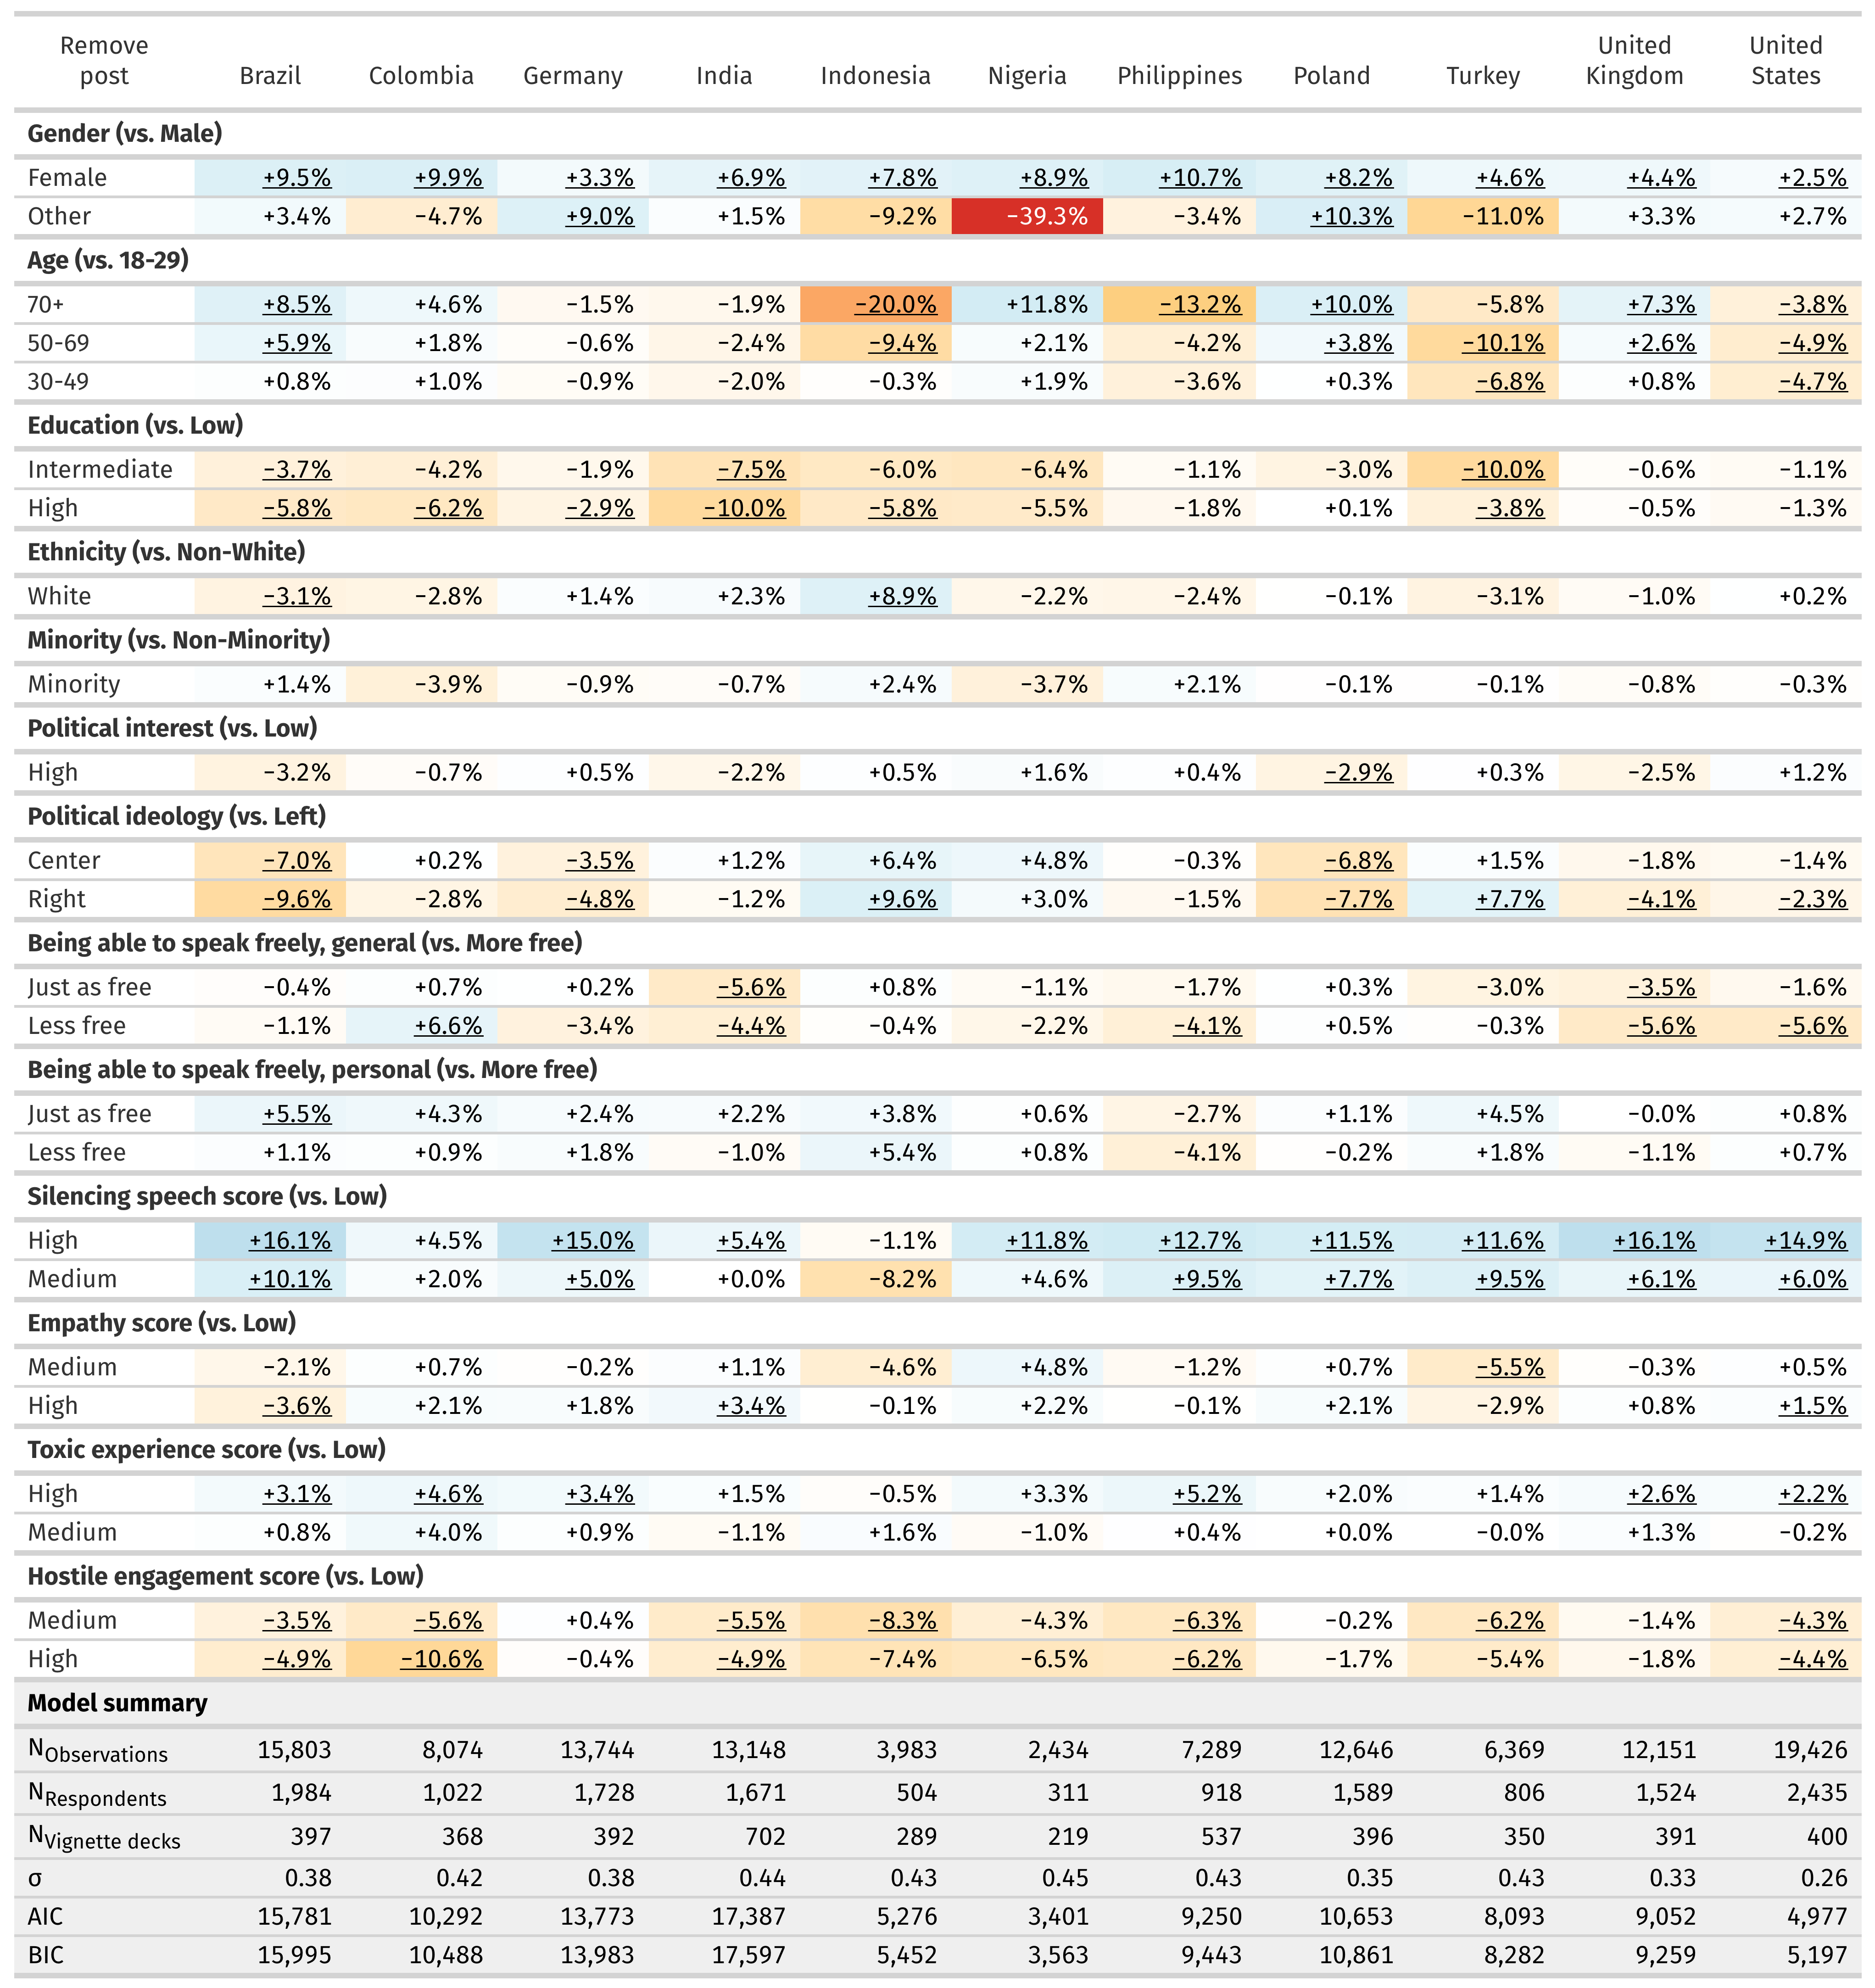
\includegraphics[width=1\linewidth]{figures/table-respmodels-vig_remove.png}
\caption{\textbf{Effects of respondent characteristics on \uline{preference for removal}, by country.\\} Estimated from hierarchical linear models with respondent and vignette deck effects. Reported estimates represent percentage-point differences in choice probabilities. Underlined estimates are significantly different from 0 with $p<0.05$. The color shading highlights the effect sizes.}
\label{fig:table-respmodels-vig_remove}
\end{figure*}

\begin{figure*}[t!]
  \centering
    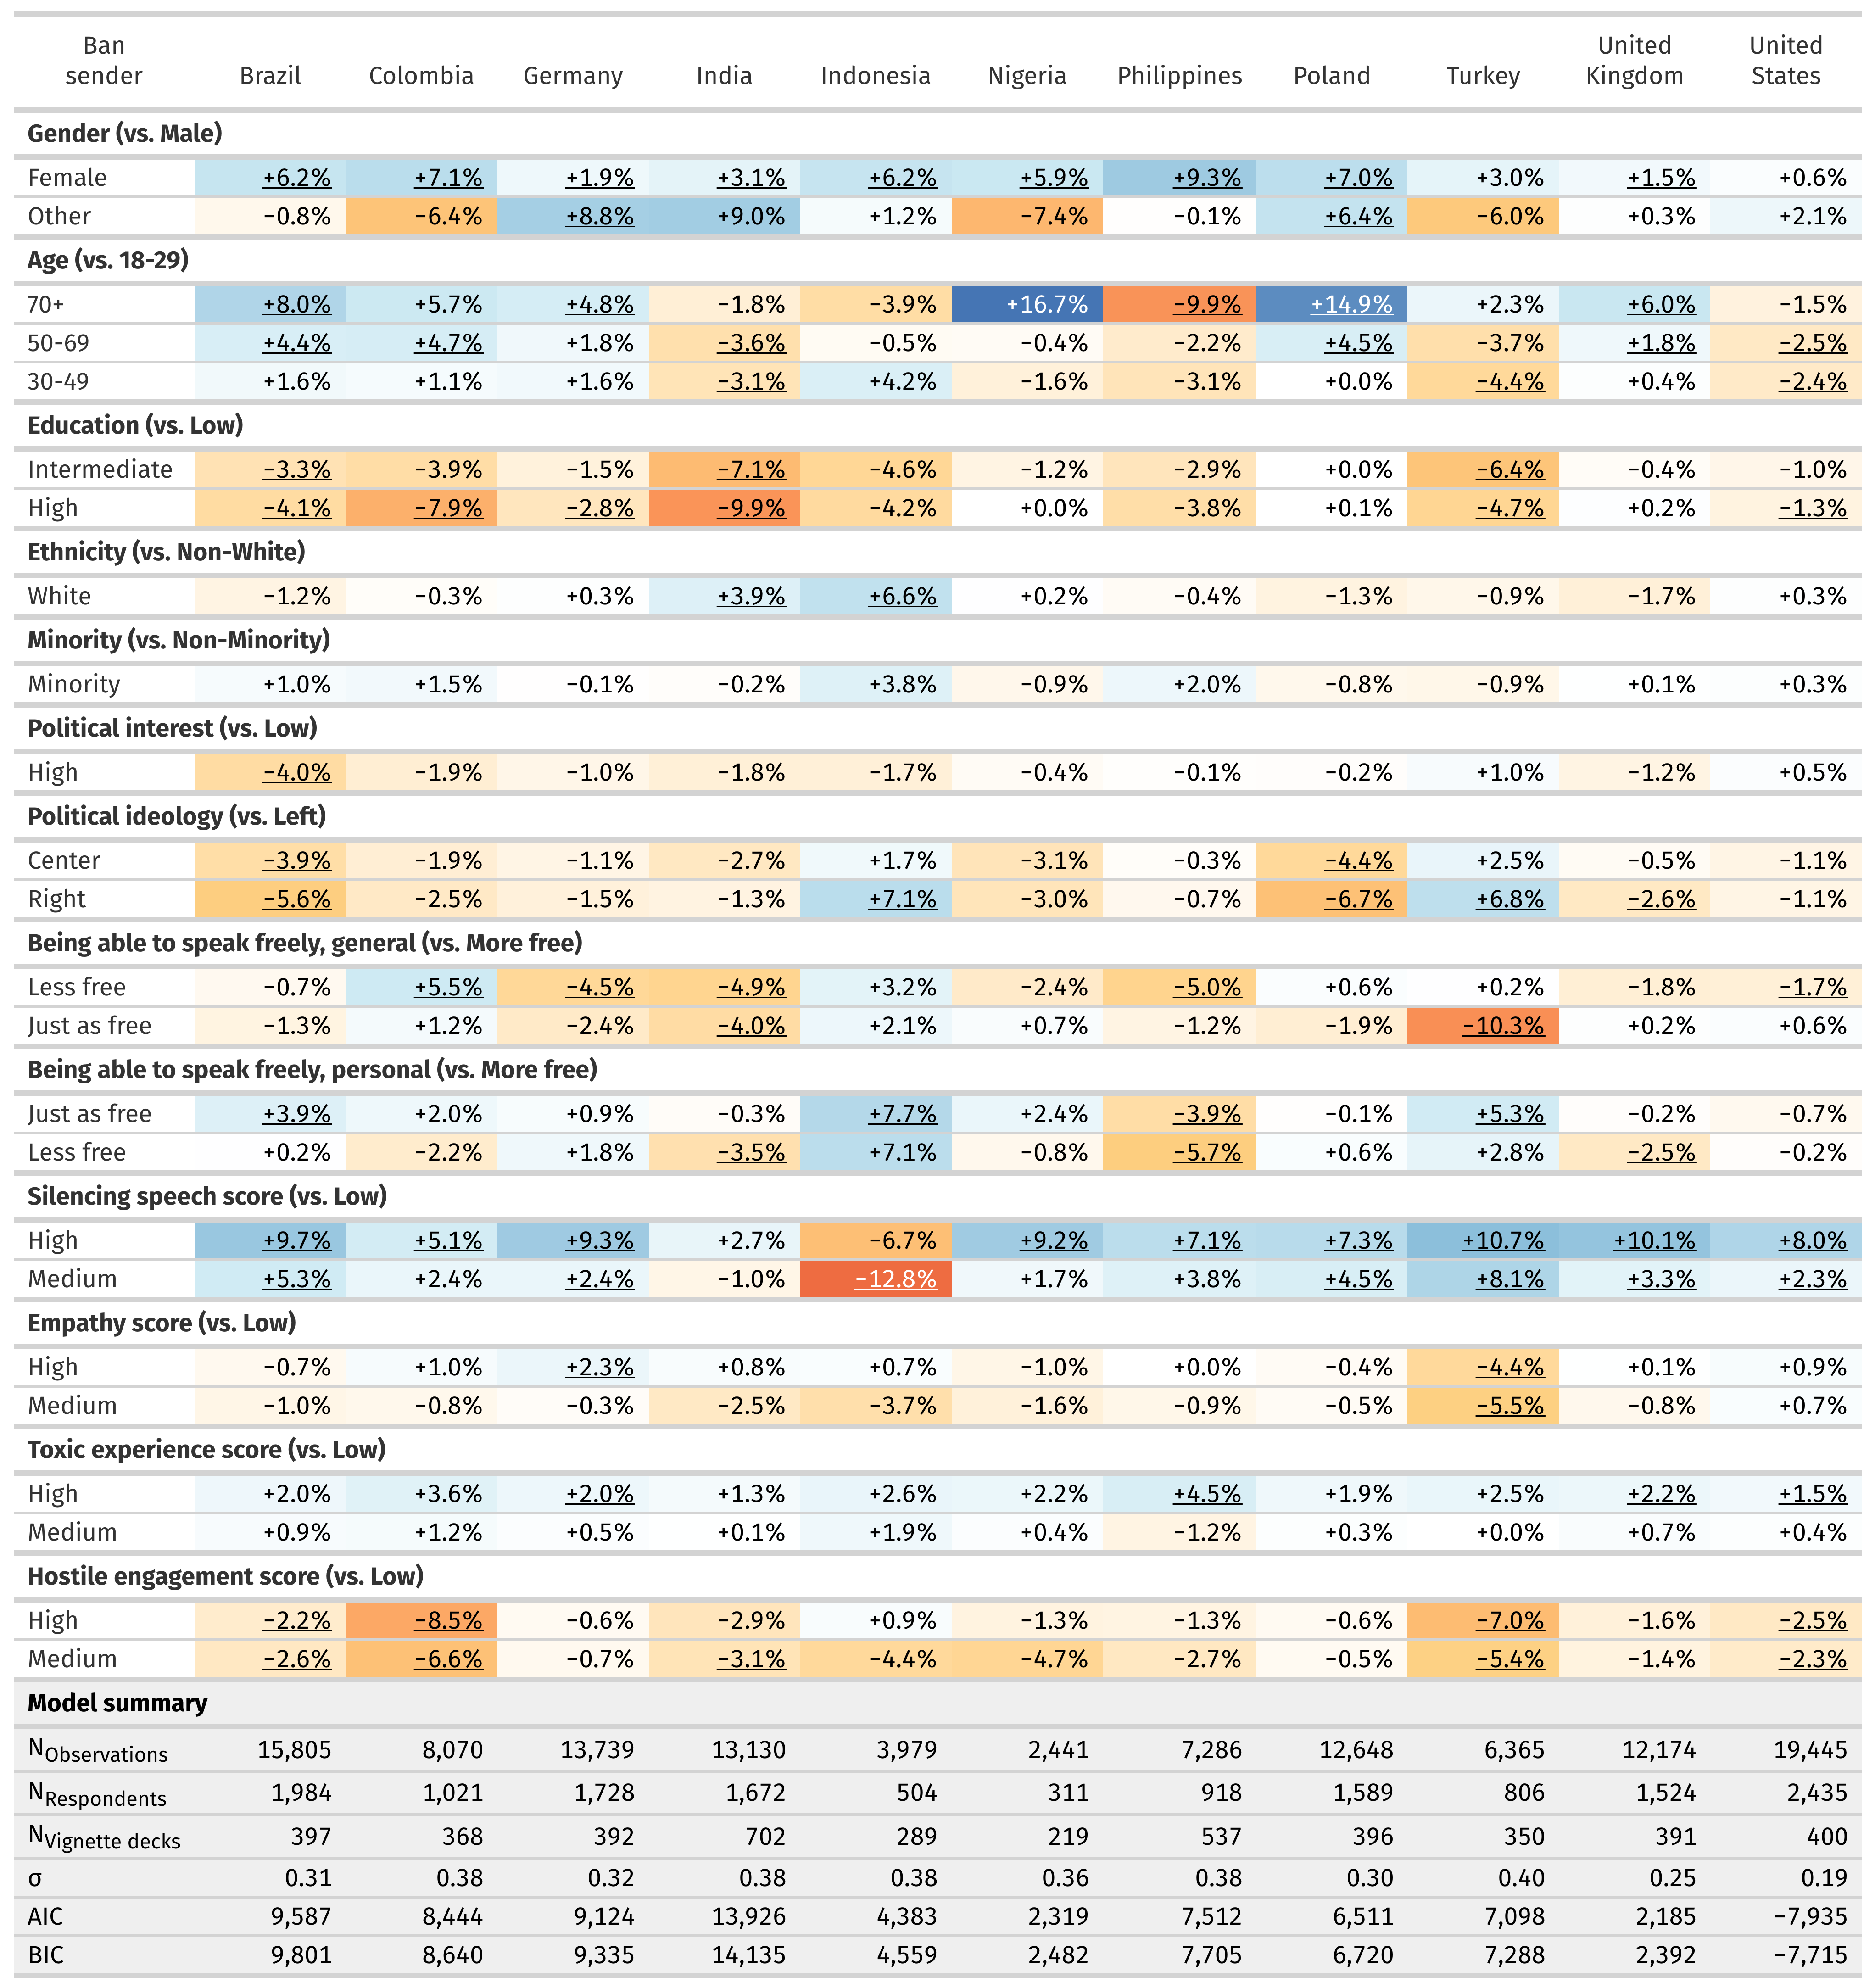
\includegraphics[width=1\linewidth]{figures/table-respmodels-vig_ban.png}
\caption{\textbf{Effects of respondent characteristics on \uline{preference for user ban}, by country.\\} Estimated from hierarchical linear models with respondent and vignette deck effects. Reported estimates represent percentage-point differences in choice probabilities. Underlined estimates are significantly different from 0 with $p<0.05$. The color shading highlights the effect sizes.}
\label{fig:table-respmodels-vig_ban}
\end{figure*}

\begin{figure*}[t!]
  \centering
    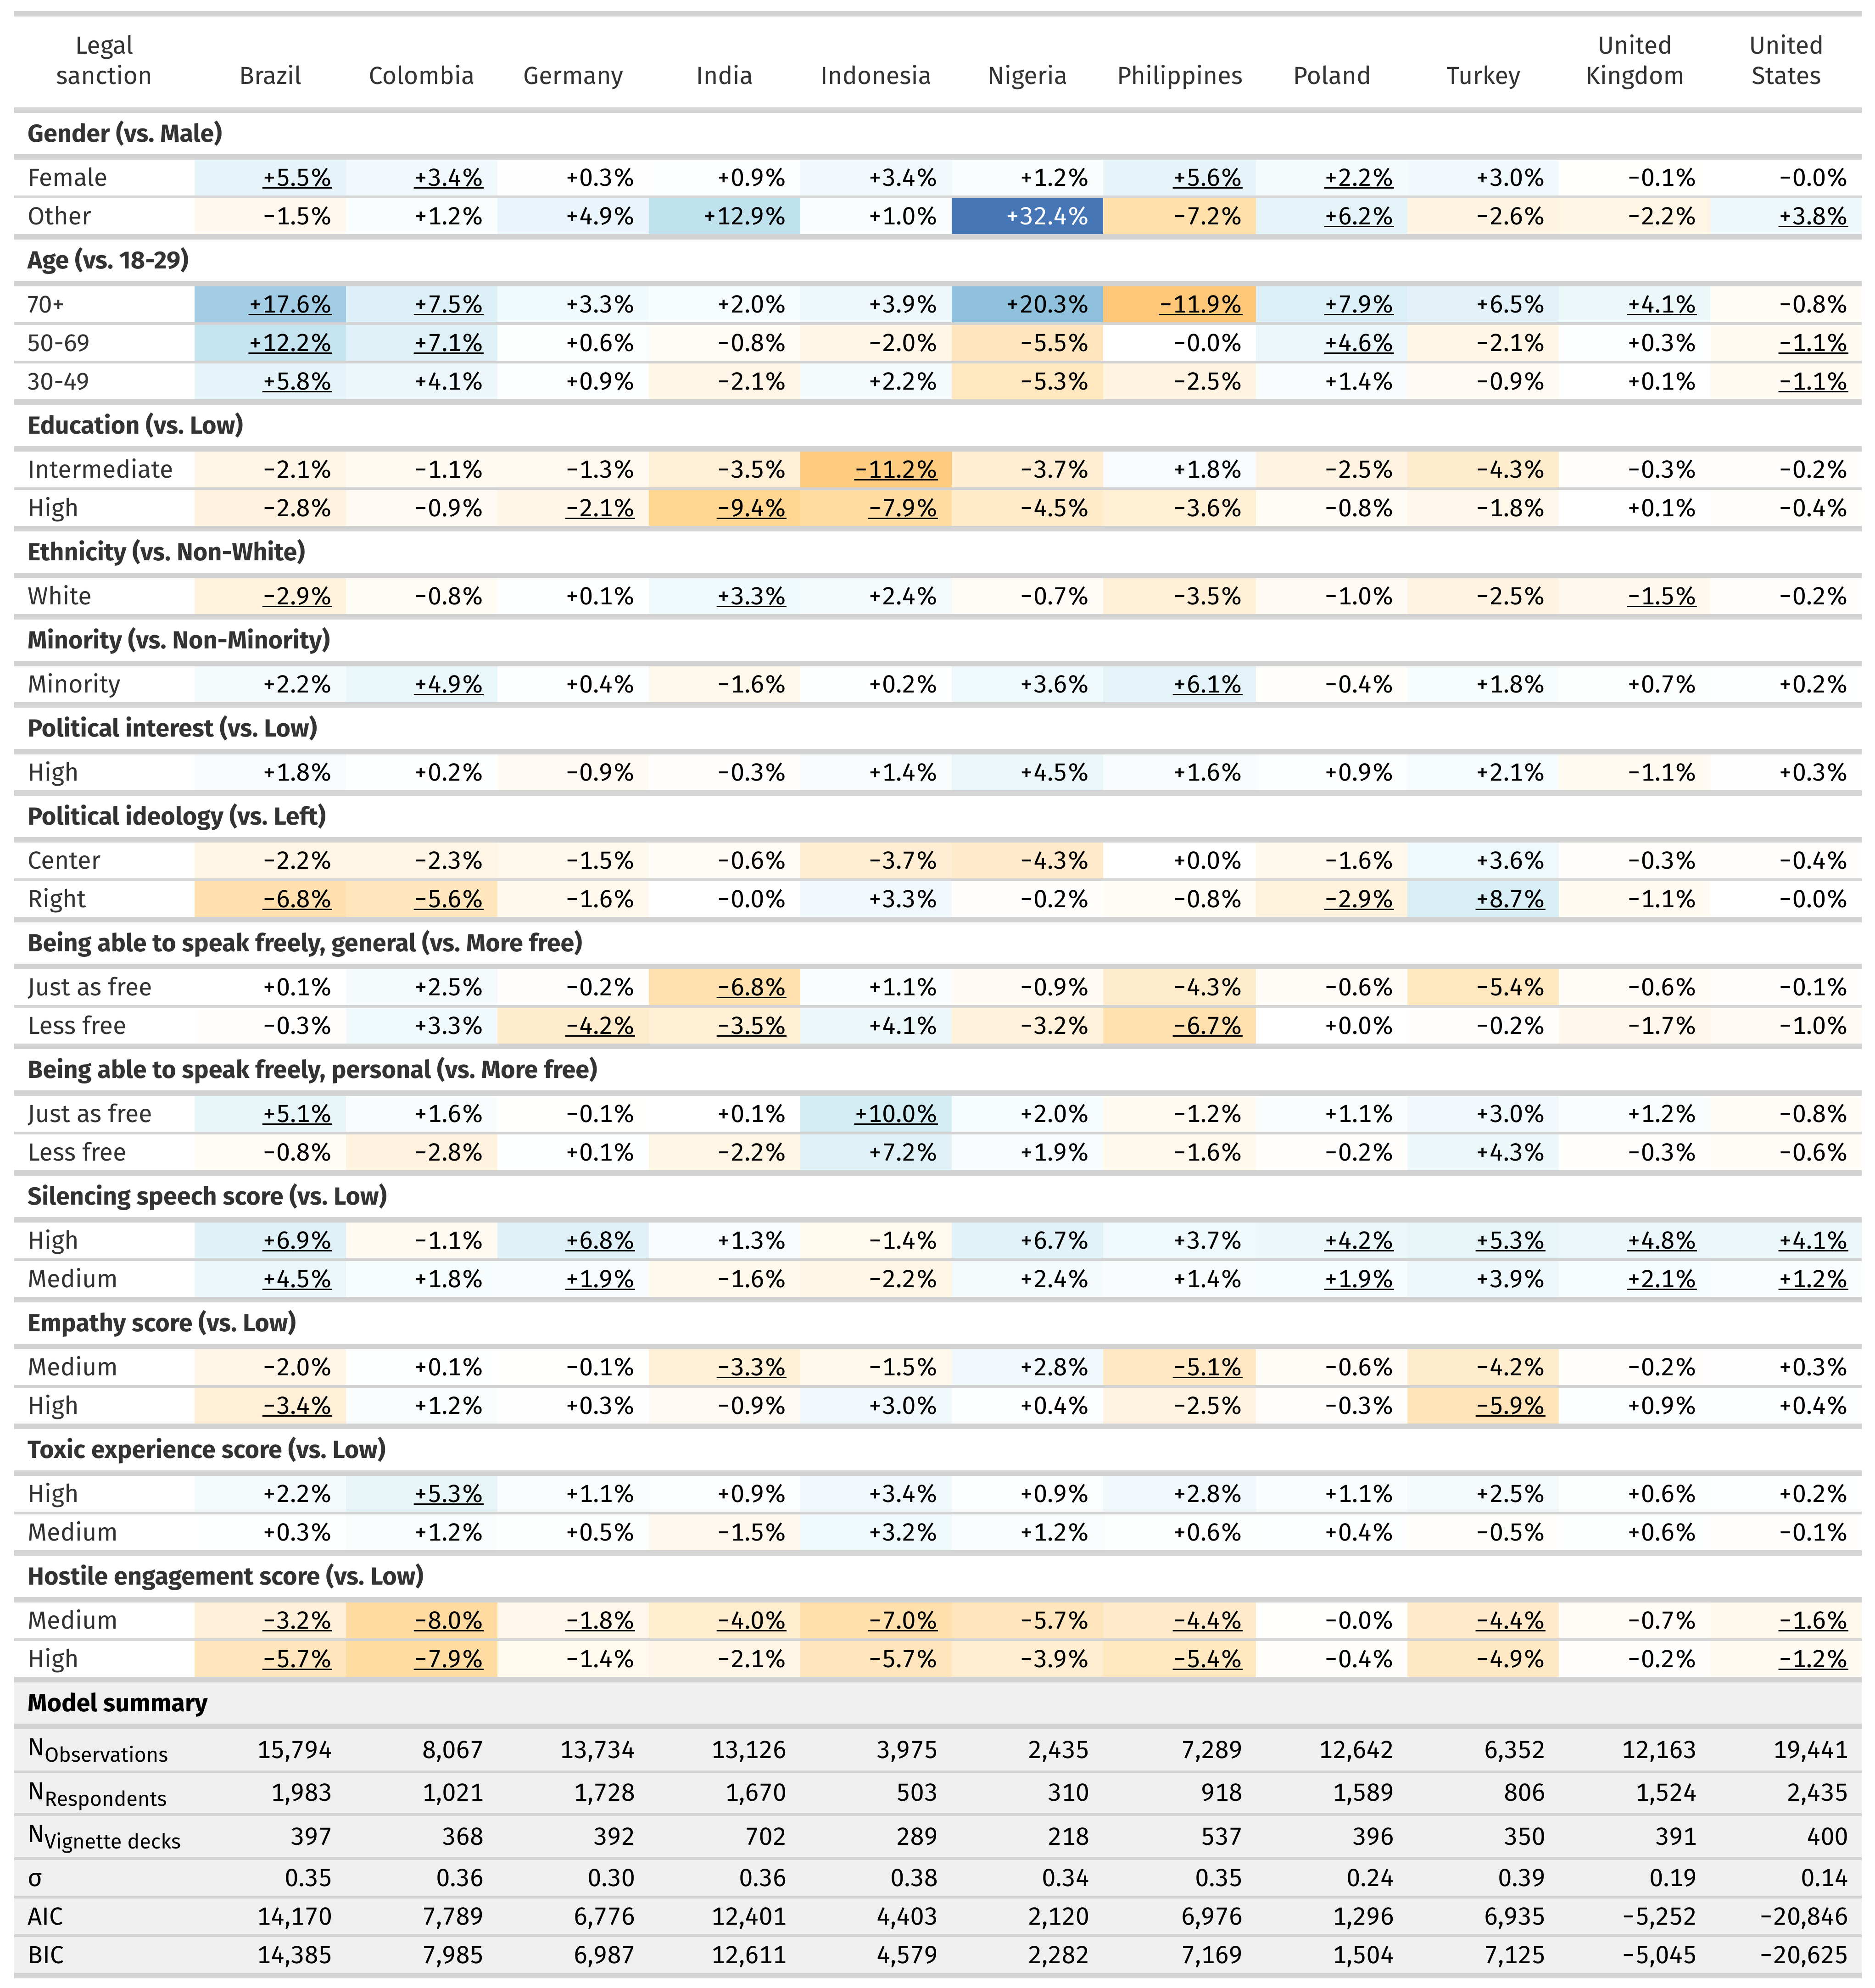
\includegraphics[width=1\linewidth]{figures/table-respmodels-vig_legal.png}
\caption{\textbf{Effects of respondent characteristics on \uline{preference for legal consequences for user}, by country.\\} Estimated from hierarchical linear models with respondent and vignette deck effects. Reported estimates represent percentage-point differences in choice probabilities. Underlined estimates are significantly different from 0 with $p<0.05$. The color shading highlights the effect sizes.}
\label{fig:table-respmodels-vig_legal}
\end{figure*}

\begin{figure*}[t!]
  \centering
    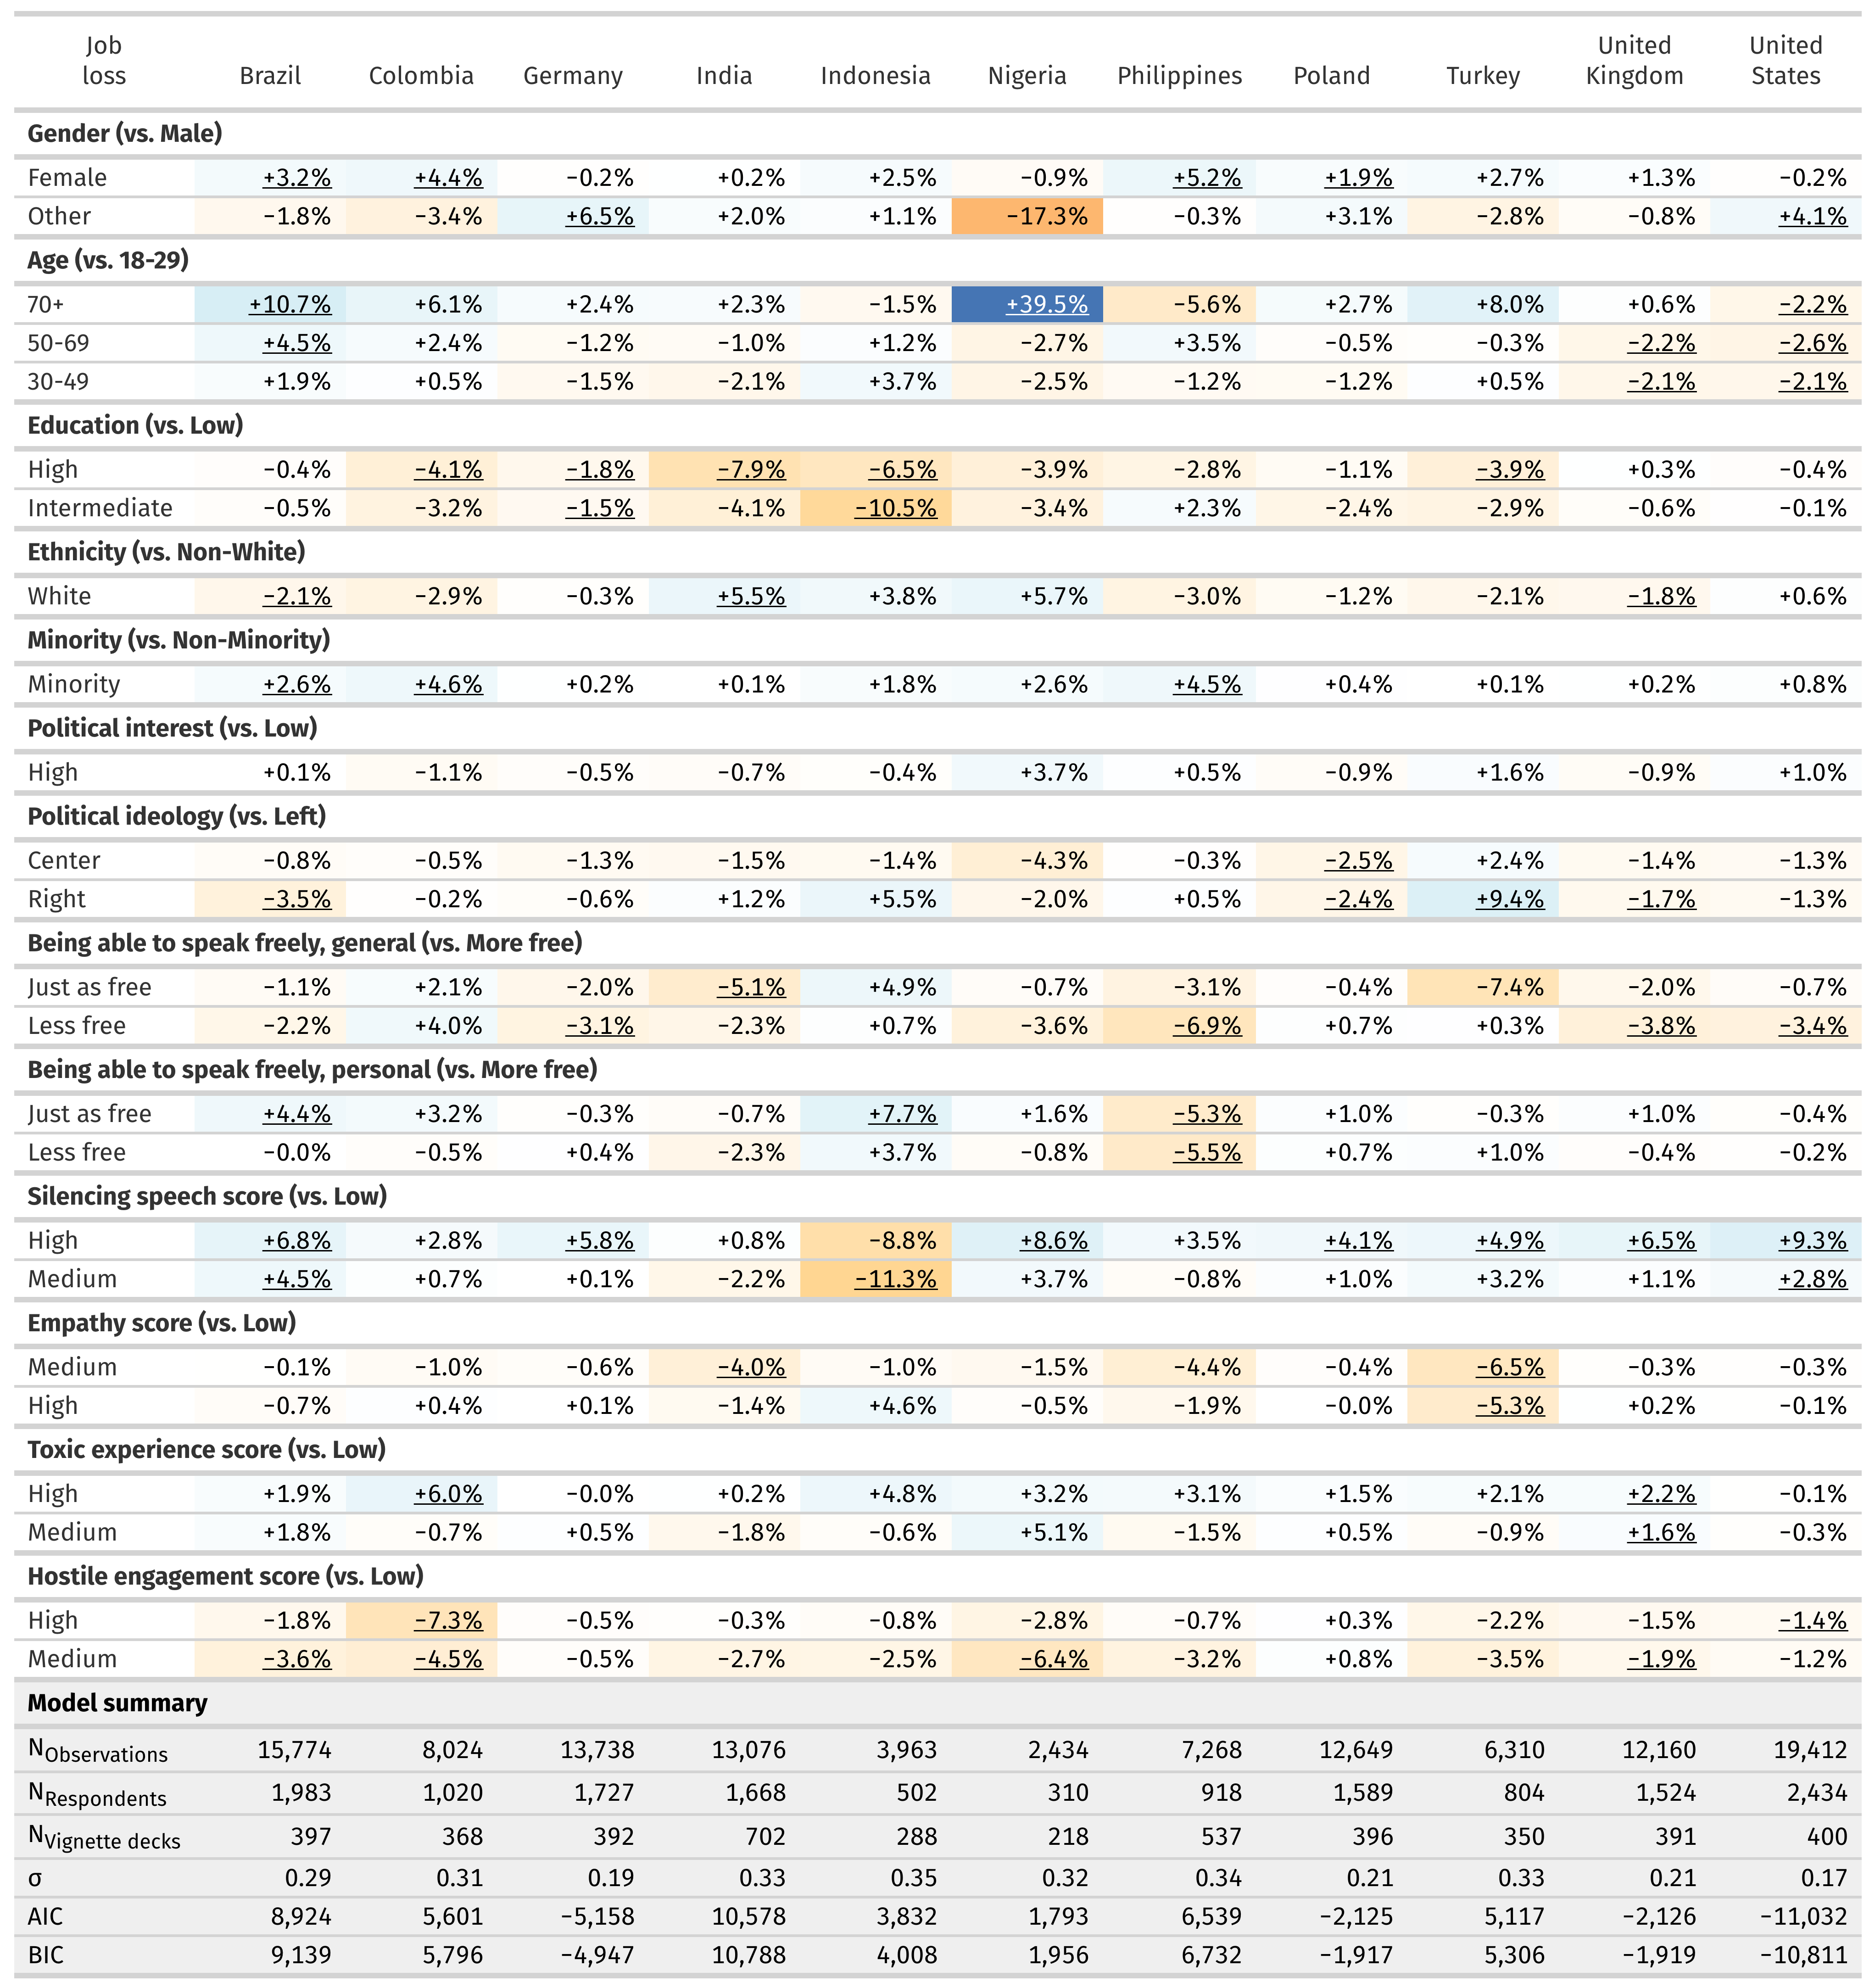
\includegraphics[width=1\linewidth]{figures/table-respmodels-vig_job.png}
\caption{\textbf{Effects of respondent characteristics on \uline{preference for job loss of user}, by country.\\} Estimated from hierarchical linear models with respondent and vignette deck effects. Reported estimates represent percentage-point differences in choice probabilities. Underlined estimates are significantly different from 0 with $p<0.05$. The color shading highlights the effect sizes.}
\label{fig:table-respmodels-vig_job}
\end{figure*}

\clearpage

\begin{table}
\begin{center}
\begin{tiny}
\begin{tabular}{l@{} D{]}{]}{19]1}@{}}
\hline
 & \multicolumn{1}{c}{Response time (s)} \\
\hline
Intercept                     & 65.49 \; [ 58.95;  72.03]^{*}  \\
Vignette position: 2          & -26.37 \; [-28.85; -23.89]^{*} \\
Vignette position: 3          & -34.10 \; [-36.58; -31.62]^{*} \\
Vignette position: 4          & -38.64 \; [-41.11; -36.16]^{*} \\
Vignette position: 5          & -40.95 \; [-43.43; -38.47]^{*} \\
Vignette position: 6          & -43.38 \; [-45.86; -40.90]^{*} \\
Vignette position: 7          & -44.45 \; [-46.93; -41.97]^{*} \\
Vignette position: 8          & -45.06 \; [-47.54; -42.58]^{*} \\
Message category: Meme        & 9.98 \; [  7.55;  12.40]^{*}   \\
Message category: Mocking     & -1.88 \; [ -4.04;   0.28]      \\
Message category: Insult      & 1.99 \; [ -0.10;   4.07]       \\
Message category: Threat      & 6.11 \; [  4.07;   8.15]^{*}   \\
Sender message length (chars) & 0.12 \; [  0.08;   0.17]^{*}   \\
Target message length (chars) & 0.05 \; [ -0.00;   0.09]       \\
\hline
Num. obs.                     & 153376                         \\
Num. groups: Respondents      & 19172                          \\
Num. groups: Decks            & 4760                           \\
Num. groups: Countries        & 11                             \\
Var: Respondents (Intercept)  & 366.27                         \\
Var: Decks (Intercept)        & 0.89                           \\
Var: Countries (Intercept)    & 81.10                          \\
Var: Residual                 & 15339.41                       \\
\hline
\multicolumn{2}{l}{\tiny{$^*$ 0 outside the confidence interval.}}
\end{tabular}
\end{tiny}
\caption{\textbf{Model of vignette response times (in seconds).} Linear mixed-effects model with person, vignette deck, and country random effects. 95\% confidence intervals in parentheses.}
\label{tab:effects-vignette-response-times-pooled}
\end{center}
\end{table}



% --------------------------------- %
\clearpage
\subsection{Framing experiment}\label{si:addresults:framing}

Here, we discuss results from the framing experiment, which was designed to test Hypotheses~H4 and~H5 (see SI section~\ref{si:exp-setup-framing}). 

Randomization appears to have worked well. All three treatment groups are of approximately equal size (around 6.4k respondents). The marginal distributions of pre-treatment covariates are balanced across all conditions (see Table~\ref{tab:balance-table-framing-experiment}).

Contrary to our expectations, neither frame affected any of the moderation outcomes (see Fig.~\ref{fig:effects-frame-by-country}). This result is remarkably stable across all outcomes and country samples. The pooled estimates are highly precise and fall near zero in nearly all cases. The only minor exception is a small, positive effect on the preference for post removal under the user protection frame ($+0.8$ pp; 95\% CI $= [0.06,\, 1.64]$; $p < 0.05$). However, this effect does not survive p-value adjustment for multiple testing.

We had pre-registered to also test the hypotheses by subsetting the sample using both a manipulation and an attention check. Specifically, we wrote:

\begin{quotation}
``The manipulation check question will be used to report, in addition to a model using the full sample, a model that is run only using treated respondents who answered the manipulation check question in accordance with their treatment condition, and all respondents in the neutral condition irrespective of how they answered the manipulation check question. The response time measure on the vignette task frame will be used to report, in addition to a model using the full sample, a model that is run only using treated respondents who spent at least 10 seconds on the survey page providing the frame.''
\end{quotation}

The manipulation check question assessed whether respondents’ perception of the platform’s mission aligned with the framing condition they received (see Fig.~\ref{fig:survey-manipcheck} for wording). However, the manipulation check indicates that the framing only weakly—if at all—affected perceptions of the platform associated with the moderation tasks (see Table~\ref{tab:frame-manipcheck}). Therefore, strong framing effects were not expected.

At the same time, responses to the manipulation check likely capture respondents’ personal beliefs about the platform’s moderation vision—shaped by their own normative attitudes. This could explain the strong associations between passing the manipulation check (i.e., perceiving the platform in line with the assigned frame) and moderation preferences (see Fig.~\ref{fig:effects-frame-by-check}). These relationships should thus not be interpreted as causal effects of framing, but rather as reflections of respondents’ pre-treatment dispositions.

When considering the pre-registered behavioral attention check (spending at least 10 seconds on the instruction page) as well as additional, exploratory checks (spending at least 25 seconds on the page or confirming that the instructions were read), no subgroup shows statistically significant or substantively meaningful framing effects.

Overall, we conclude that our results do not provide evidence for Hypotheses~H4 and~H5, i.e., for any framing effects. This partially replicates findings from \cite{munzertCitizenPreferencesOnline2025}, where two similarly constructed frames slightly reduced perceptions of offensiveness and hatefulness but otherwise had little impact on preferences.

It is important to note that framing may still occur in real-world contexts. Our experiment does not speak to potential effects of platform moderation guidelines, moderation cultures, or broader contextual and cultural influences.  What we demonstrate is that the specific platform framing manipulations used here had no detectable effect on moderation decisions, which is consistent with but does not conclusively establish the general robustness of moderation judgments to contextual framing.


Finally, these findings suggest that the results of our other experiments are unlikely to be driven by framing effects. From a design perspective, this is reassuring, as it implies that our main findings are robust to alternative framings. In this sense, the framing experiment provides additional support for the overall validity of the moderation experiment.


\begin{table}
\centering
\begin{talltblr}[         %% tabularray outer open
caption={Descriptive statistics of respondent characteristics, by treatment group status (framing experiment)\label{tab:balance-table-framing-experiment}},
]                     %% tabularray outer close
{                     %% tabularray inner open
colspec={Q[]Q[]Q[]Q[]Q[]Q[]Q[]Q[]},
cell{2}{1}={}{halign=l,},
cell{2}{2}={}{halign=l,},
cell{3}{1}={}{halign=l,},
cell{3}{2}={}{halign=l,},
cell{4}{1}={}{halign=l,},
cell{4}{2}={}{halign=l,},
cell{5}{1}={}{halign=l,},
cell{5}{2}={}{halign=l,},
cell{6}{1}={}{halign=l,},
cell{6}{2}={}{halign=l,},
cell{7}{1}={}{halign=l,},
cell{7}{2}={}{halign=l,},
cell{8}{1}={}{halign=l,},
cell{8}{2}={}{halign=l,},
cell{9}{1}={}{halign=l,},
cell{9}{2}={}{halign=l,},
cell{10}{1}={}{halign=l,},
cell{10}{2}={}{halign=l,},
cell{11}{1}={}{halign=l,},
cell{11}{2}={}{halign=l,},
cell{12}{1}={}{halign=l,},
cell{12}{2}={}{halign=l,},
cell{13}{1}={}{halign=l,},
cell{13}{2}={}{halign=l,},
cell{14}{1}={}{halign=l,},
cell{14}{2}={}{halign=l,},
cell{15}{1}={}{halign=l,},
cell{15}{2}={}{halign=l,},
cell{16}{1}={}{halign=l,},
cell{16}{2}={}{halign=l,},
cell{1}{1}={}{halign=l, halign=c,},
cell{1}{2}={}{halign=l, halign=c,},
cell{2}{3}={}{halign=r,},
cell{2}{4}={}{halign=r,},
cell{2}{5}={}{halign=r,},
cell{2}{6}={}{halign=r,},
cell{2}{7}={}{halign=r,},
cell{2}{8}={}{halign=r,},
cell{3}{3}={}{halign=r,},
cell{3}{4}={}{halign=r,},
cell{3}{5}={}{halign=r,},
cell{3}{6}={}{halign=r,},
cell{3}{7}={}{halign=r,},
cell{3}{8}={}{halign=r,},
cell{4}{3}={}{halign=r,},
cell{4}{4}={}{halign=r,},
cell{4}{5}={}{halign=r,},
cell{4}{6}={}{halign=r,},
cell{4}{7}={}{halign=r,},
cell{4}{8}={}{halign=r,},
cell{5}{3}={}{halign=r,},
cell{5}{4}={}{halign=r,},
cell{5}{5}={}{halign=r,},
cell{5}{6}={}{halign=r,},
cell{5}{7}={}{halign=r,},
cell{5}{8}={}{halign=r,},
cell{6}{3}={}{halign=r,},
cell{6}{4}={}{halign=r,},
cell{6}{5}={}{halign=r,},
cell{6}{6}={}{halign=r,},
cell{6}{7}={}{halign=r,},
cell{6}{8}={}{halign=r,},
cell{7}{3}={}{halign=r,},
cell{7}{4}={}{halign=r,},
cell{7}{5}={}{halign=r,},
cell{7}{6}={}{halign=r,},
cell{7}{7}={}{halign=r,},
cell{7}{8}={}{halign=r,},
cell{8}{3}={}{halign=r,},
cell{8}{4}={}{halign=r,},
cell{8}{5}={}{halign=r,},
cell{8}{6}={}{halign=r,},
cell{8}{7}={}{halign=r,},
cell{8}{8}={}{halign=r,},
cell{9}{3}={}{halign=r,},
cell{9}{4}={}{halign=r,},
cell{9}{5}={}{halign=r,},
cell{9}{6}={}{halign=r,},
cell{9}{7}={}{halign=r,},
cell{9}{8}={}{halign=r,},
cell{10}{3}={}{halign=r,},
cell{10}{4}={}{halign=r,},
cell{10}{5}={}{halign=r,},
cell{10}{6}={}{halign=r,},
cell{10}{7}={}{halign=r,},
cell{10}{8}={}{halign=r,},
cell{11}{3}={}{halign=r,},
cell{11}{4}={}{halign=r,},
cell{11}{5}={}{halign=r,},
cell{11}{6}={}{halign=r,},
cell{11}{7}={}{halign=r,},
cell{11}{8}={}{halign=r,},
cell{12}{3}={}{halign=r,},
cell{12}{4}={}{halign=r,},
cell{12}{5}={}{halign=r,},
cell{12}{6}={}{halign=r,},
cell{12}{7}={}{halign=r,},
cell{12}{8}={}{halign=r,},
cell{13}{3}={}{halign=r,},
cell{13}{4}={}{halign=r,},
cell{13}{5}={}{halign=r,},
cell{13}{6}={}{halign=r,},
cell{13}{7}={}{halign=r,},
cell{13}{8}={}{halign=r,},
cell{14}{3}={}{halign=r,},
cell{14}{4}={}{halign=r,},
cell{14}{5}={}{halign=r,},
cell{14}{6}={}{halign=r,},
cell{14}{7}={}{halign=r,},
cell{14}{8}={}{halign=r,},
cell{15}{3}={}{halign=r,},
cell{15}{4}={}{halign=r,},
cell{15}{5}={}{halign=r,},
cell{15}{6}={}{halign=r,},
cell{15}{7}={}{halign=r,},
cell{15}{8}={}{halign=r,},
cell{16}{3}={}{halign=r,},
cell{16}{4}={}{halign=r,},
cell{16}{5}={}{halign=r,},
cell{16}{6}={}{halign=r,},
cell{16}{7}={}{halign=r,},
cell{16}{8}={}{halign=r,},
cell{1}{4}={}{halign=r, halign=c,},
cell{1}{6}={}{halign=r, halign=c,},
cell{1}{8}={}{halign=r, halign=c,},
cell{1}{3}={c=2,}{halign=r, halign=c, halign=c,},
cell{1}{5}={c=2,}{halign=r, halign=c, halign=c,},
cell{1}{7}={c=2,}{halign=r, halign=c, halign=c,},
}                     %% tabularray inner close
\toprule
&  & Neutral (N=6478) &  & Free speech (N=6328) &  & Protect users (N=6366) &  \\ \cmidrule[lr]{3-4}\cmidrule[lr]{5-6}\cmidrule[lr]{7-8}
&    & N & Pct. & N & Pct. & N & Pct. \\ \midrule %% TinyTableHeader
Gender & Male & \num{4158} & \num{64.2} & \num{4086} & \num{64.6} & \num{4068} & \num{63.9} \\
& Female & \num{2195} & \num{33.9} & \num{2122} & \num{33.5} & \num{2162} & \num{34.0} \\
& Other & \num{125} & \num{1.9} & \num{120} & \num{1.9} & \num{136} & \num{2.1} \\
Age & 18-29 & \num{1578} & \num{24.4} & \num{1578} & \num{24.9} & \num{1533} & \num{24.1} \\
& 30-49 & \num{2365} & \num{36.5} & \num{2277} & \num{36.0} & \num{2290} & \num{36.0} \\
& 50-69 & \num{2176} & \num{33.6} & \num{2094} & \num{33.1} & \num{2130} & \num{33.5} \\
& 70+ & \num{348} & \num{5.4} & \num{364} & \num{5.8} & \num{392} & \num{6.2} \\
Education & Low & \num{1415} & \num{21.8} & \num{1405} & \num{22.2} & \num{1341} & \num{21.1} \\
& Intermediate & \num{1373} & \num{21.2} & \num{1297} & \num{20.5} & \num{1297} & \num{20.4} \\
& High & \num{3690} & \num{57.0} & \num{3626} & \num{57.3} & \num{3728} & \num{58.6} \\
Ethnicity & Non-White & \num{2694} & \num{41.6} & \num{2581} & \num{40.8} & \num{2598} & \num{40.8} \\
& White & \num{3462} & \num{53.4} & \num{3474} & \num{54.9} & \num{3465} & \num{54.4} \\
Minority & Non-Minority & \num{4351} & \num{67.2} & \num{4266} & \num{67.4} & \num{4255} & \num{66.8} \\
& Minority & \num{2094} & \num{32.3} & \num{2020} & \num{31.9} & \num{2056} & \num{32.3} \\
\bottomrule
\end{talltblr}
\end{table}


\input{figures/frame-manipcheck.tex}

\begin{figure*}[h!]
  \centering
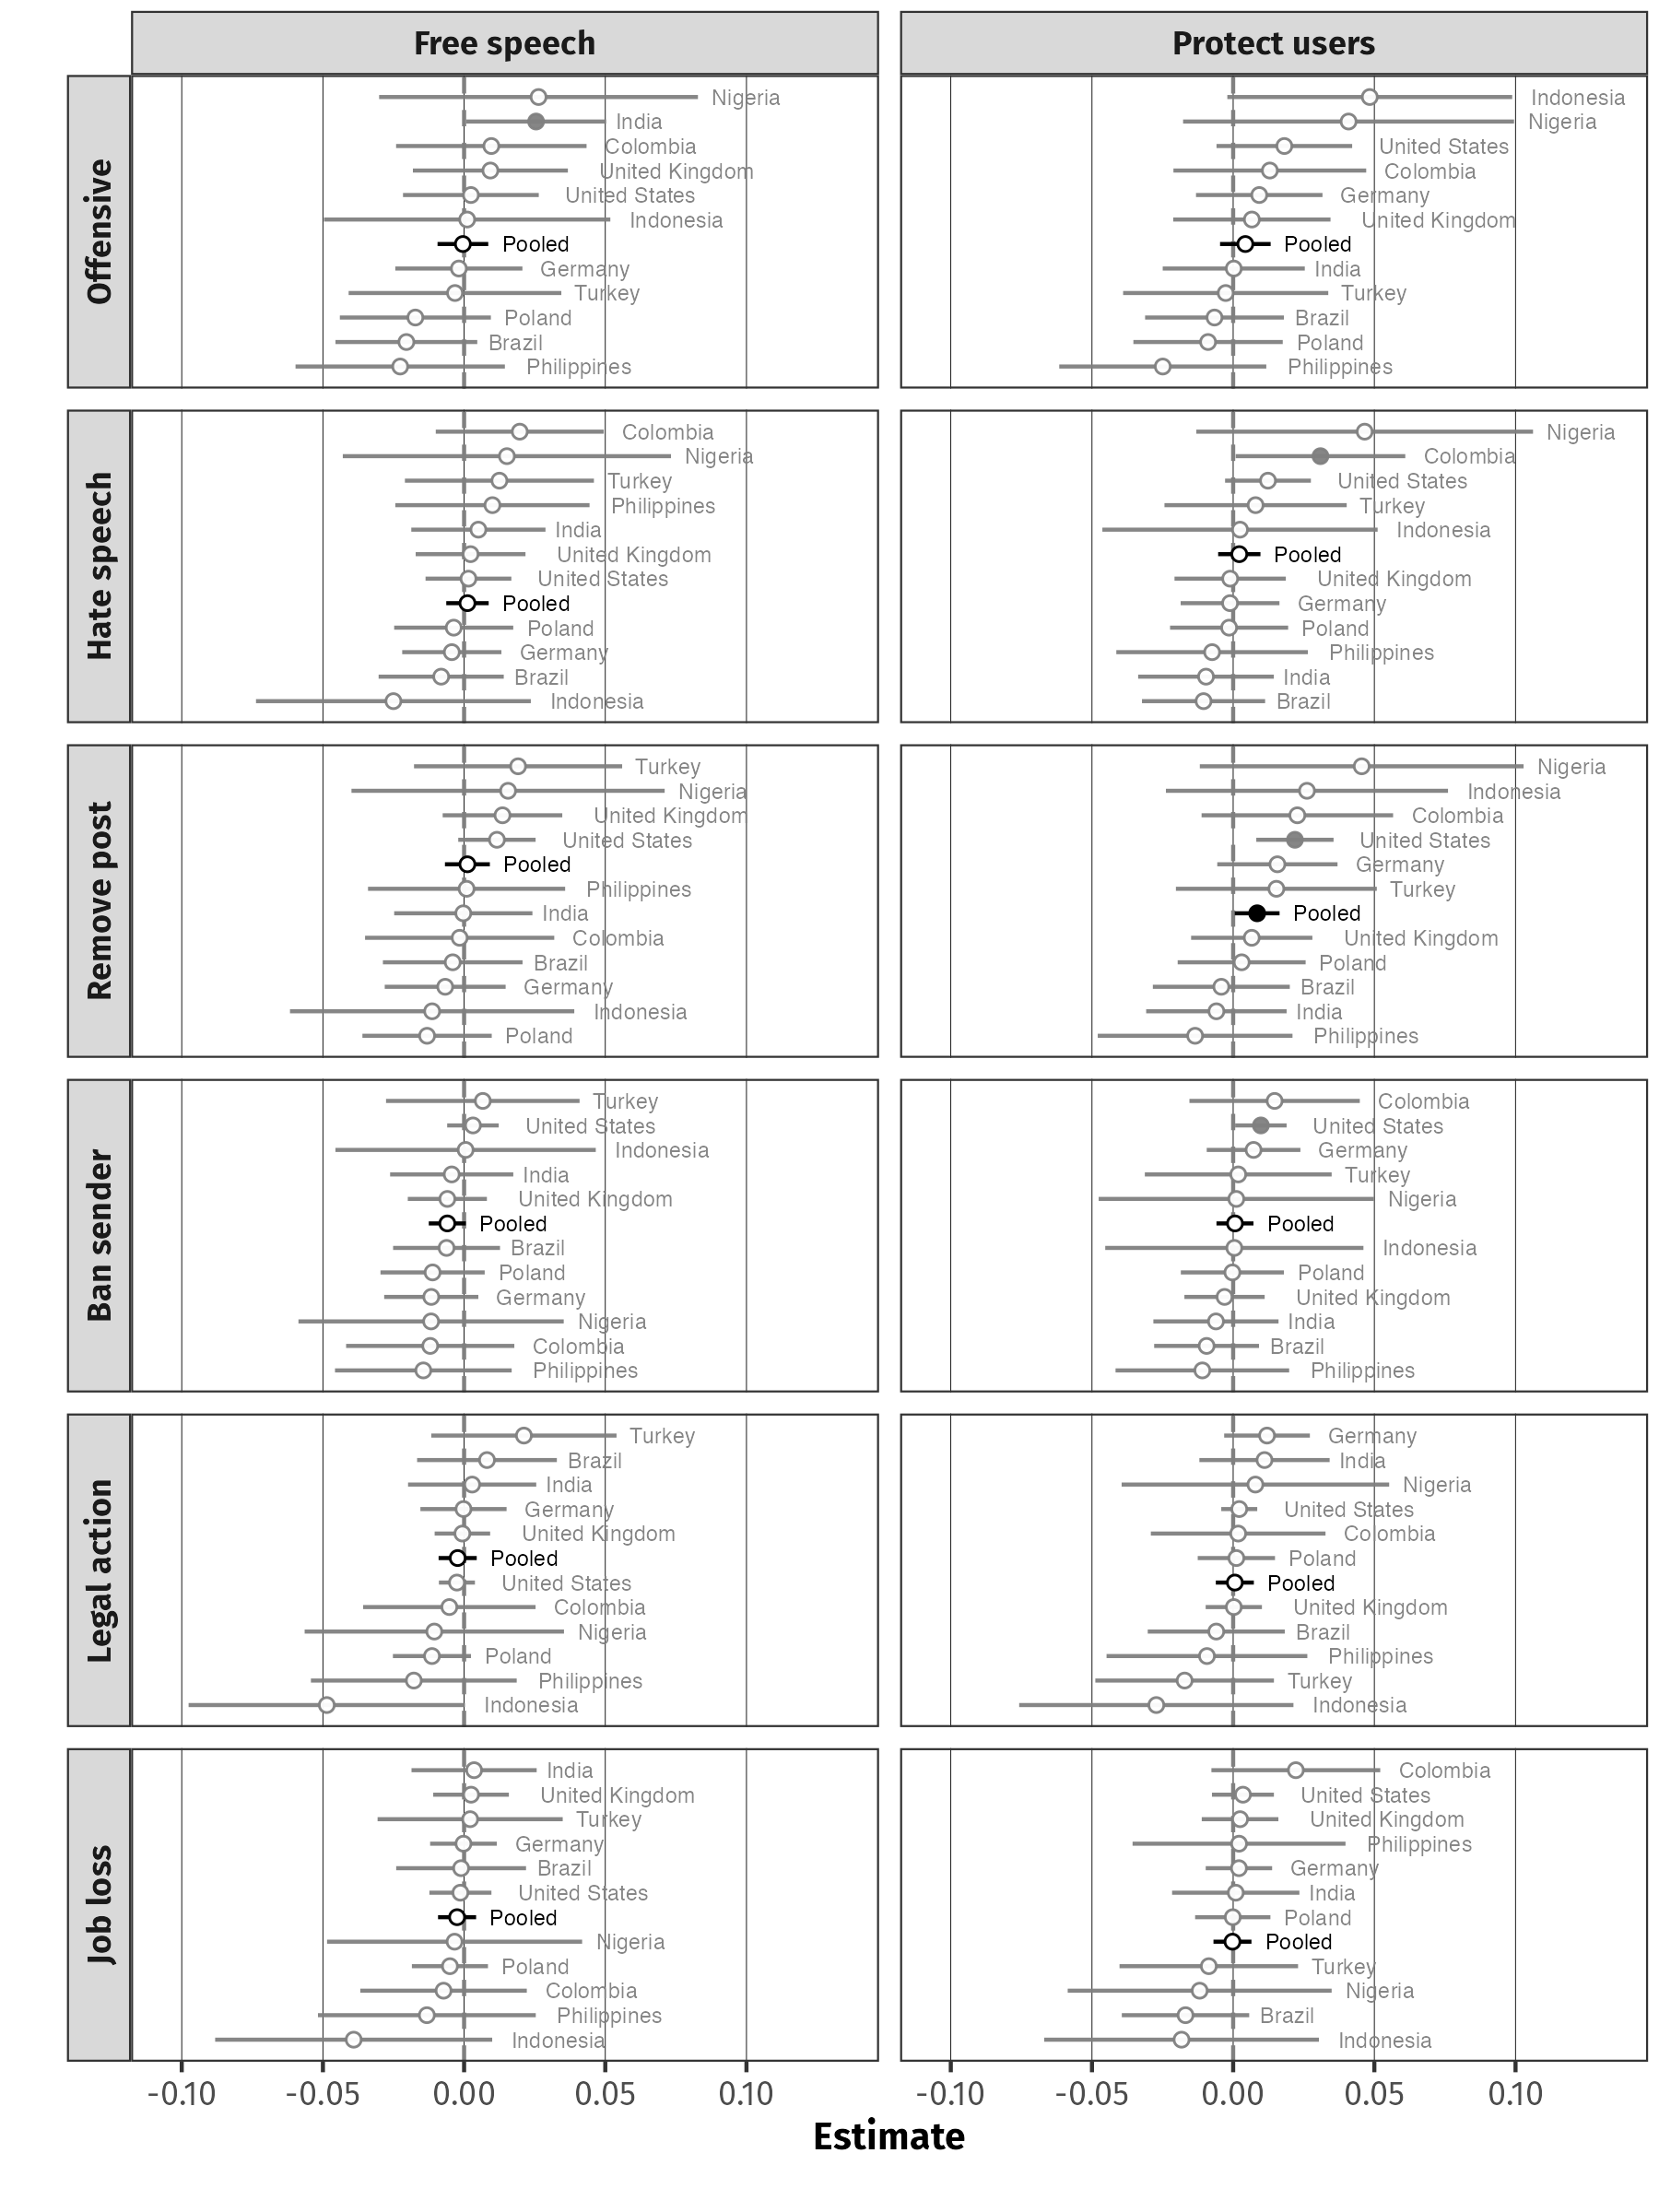
\includegraphics[width=.9\linewidth]{figures/effects-frame-by-country.png}
\caption{\textbf{Effects of free speech and user protection frames (vs. neutral frame) on moderation outcomes, by country.} Error bars represent 95\% confidence intervals. Filled circles indicate that the effect remains significant after p-value adjustment by controlling the false discovery rate.}
\label{fig:effects-frame-by-country}
\end{figure*}

\begin{figure*}[t!]
  \centering
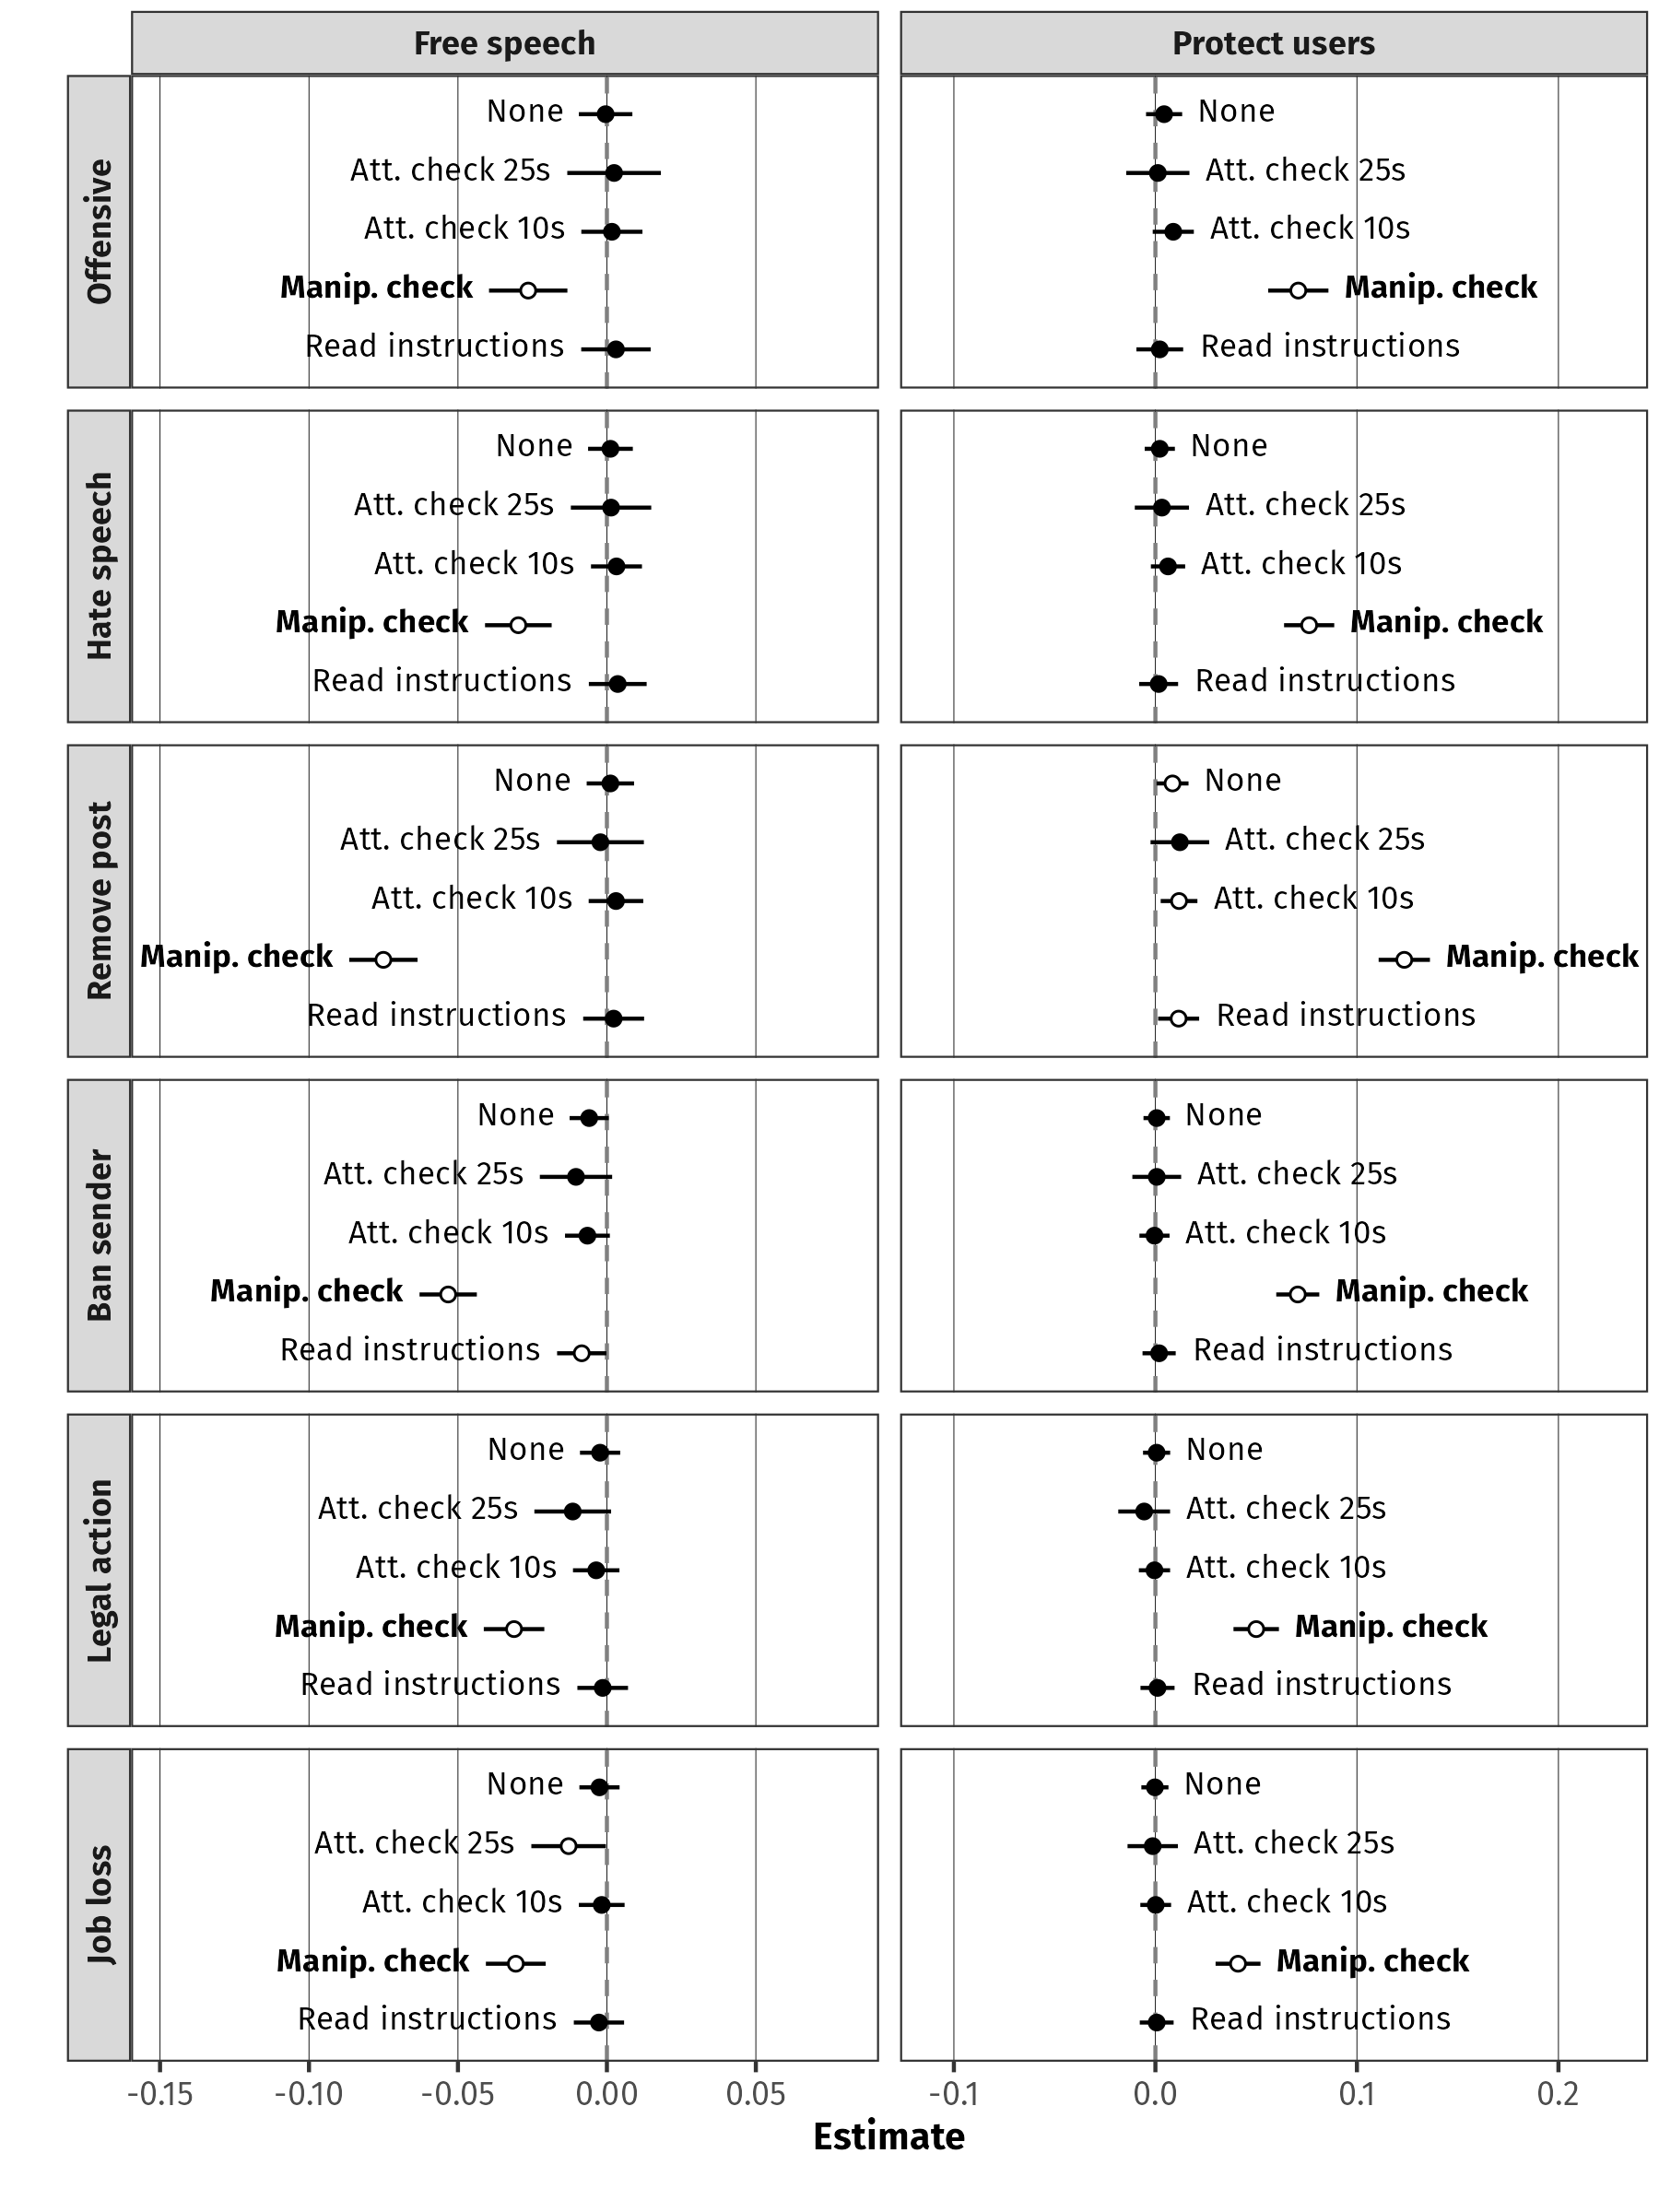
\includegraphics[width=.9\linewidth]{figures/effects-frame-by-check.png}
\caption{\textbf{Effects of free speech and user protection frames (vs. neutral frame) on moderation outcomes, by attention/manipulation check criterion.} Error bars represent 95\% confidence intervals. Filled circles indicate that the effect remains significant after p-value adjustment by controlling the false discovery rate.}
\label{fig:effects-frame-by-check}
\end{figure*}


% --------------------------------- %
\clearpage
\subsection{Exposure experiment}\label{si:addresults:exposure}

Here, we discuss results from the exposure experiment, which was designed to test Hypothesis~H6 (see SI section~\ref{si:exp-setup-exposure}). 

Randomization appears to have worked well. The treatment groups are of comparable size, and the marginal distributions of pre-treatment covariates are balanced across all conditions (see Table~\ref{tab:balance-table-exposure-experiment}).

Figure~\ref{fig:effects-exposure-none} presents the estimated effects by outcome. Overall, our expectations were largely confirmed. Exposure to toxic speech increased perceptions of responsibility, particularly for employers, where the effect is especially pronounced ($+0.33~\text{scale points}$; $\text{95\% CI} = 0.30; 0.37$; $P < 0.001$)). The only exception is the case of social platforms, for which we find no evidence of an effect—except in the Polish sample, where the effect is negative.

Regarding the trade-offs, attitudes reflecting a pro–free-speech stance are somewhat dampened after exposure. Support for the statement “People should be allowed to express unpopular opinions in public, even those that are deeply offensive to other people” decreases slightly ($-0.02~\text{scale points}$; $\text{95\% CI} = -0.04; -0.01$; $P < 0.001$)), as does support for the statement “People should be able to speak their minds freely online” ($-0.03~\text{scale points}$; $\text{95\% CI} = -0.06; -0.01$; $P < 0.01$)). The effect on support for the statement “Online services have a responsibility to step in when harassing behavior occurs on their site” is not statistically distinguishable from zero ($+0.01~\text{scale points}$; $\text{95\% CI} = -0.00; 0.02$; $P = 0.09$)).

Overall, these findings partially replicate those of \cite{munzertCitizenPreferencesOnline2025}, who also observed a dampening effect on support for the free expression of unpopular opinions.

\input{figures/balance-table-exposure-experiment}

\begin{figure*}[h!]
  \centering
    \includegraphics[width=.9\linewidth]{figures/effects-exposure-none.png}
\caption{\textbf{Estimated effects of speech vignette exposure on selected attitudes and preferences.} Error bars represent 95\% confidence intervals. Filled circles indicate that the effect remains significant after p-value adjustment by controlling the false discovery rate. Responsibility perceptions measured on 4-point scale. Trade-offs measured on binary scale.}
\label{fig:effects-exposure-none}
\end{figure*}




% --------------------------------- %
\clearpage
\subsection{Synthetic social media posts}\label{si:posts}

% --------------------------------- %
\subsubsection{Target messages}\label{si:posts:targetmessages}

\input{figures/target-messages.tex}


% --------------------------------- %
\clearpage
\subsubsection{Sender messages}\label{si:posts:sendermessages}

\begin{landscape}
\input{figures/sender-messages-suvdrivers.tex}
\end{landscape}

\begin{landscape}
\input{figures/sender-messages-police.tex}
\end{landscape}

\begin{landscape}
\input{figures/sender-messages-nationalism.tex}
\end{landscape}

\begin{landscape}
\input{figures/sender-messages-inequality.tex}
\end{landscape}

\begin{landscape}
\input{figures/sender-messages-religiosity.tex}
\end{landscape}

\begin{landscape}
\input{figures/sender-messages-homosexuality.tex}
\end{landscape}

\begin{landscape}
\input{figures/sender-messages-partisanship.tex}
\end{landscape}

\begin{landscape}
\input{figures/sender-messages-freespeech.tex}
\end{landscape}

\begin{landscape}
\input{figures/sender-messages-climatechange.tex}
\end{landscape}

\begin{landscape}
\input{figures/sender-messages-veganism.tex}
\end{landscape}

\begin{landscape}
\input{figures/sender-messages-racism.tex}
\end{landscape}

\begin{landscape}
\input{figures/sender-messages-immigration.tex}
\end{landscape}

\begin{landscape}
\input{figures/sender-messages-mensrights.tex}
\end{landscape}

\begin{landscape}
\input{figures/sender-messages-feminism.tex}
\end{landscape}


% --------------------------------- %
\subsection{Sender memes}\label{si:posts:sendermemes}

% ---------- SUV drivers ----------
\begin{figure*}[t!hb]
  \centering
  \setlength{\fboxsep}{2pt}
  \fbox{%
    \begin{minipage}{0.95\linewidth}
      \centering
      \begin{subfigure}[b]{0.48\linewidth}
        \includegraphics[width=\linewidth]{figures/memes-usa/cars_l_group_usa.jpeg}
        \caption{ Right-leaning, group framing}
      \end{subfigure}
      \hfill
      \begin{subfigure}[b]{0.48\linewidth}
        \includegraphics[width=\linewidth]{figures/memes-usa/cars_l_personal_usa.jpeg}
        \caption{ Right-leaning, personal framing}
      \end{subfigure}
      \\[6pt]
      \begin{subfigure}[b]{0.48\linewidth}
        \includegraphics[width=\linewidth]{figures/memes-usa/cars_r_group_usa.jpeg}
        \caption{ Left-leaning, group framing}
      \end{subfigure}
      \hfill
      \begin{subfigure}[b]{0.48\linewidth}
        \includegraphics[width=\linewidth]{figures/memes-usa/cars_r_personal_usa.jpeg}
        \caption{ Left-leaning, personal framing}
      \end{subfigure}
    \end{minipage}%
  }
  \caption{\textbf{Memes, U.S. sample.} Topic: SUV drivers}
\end{figure*}

% ---------- Climate change ----------
\begin{figure*}[t!hb]
  \centering
  \setlength{\fboxsep}{2pt}
  \fbox{%
    \begin{minipage}{0.95\linewidth}
      \centering
      \begin{subfigure}[b]{0.48\linewidth}
        \includegraphics[width=\linewidth]{figures/memes-usa/climate_l_group_usa.jpeg}
        \caption{ Right-leaning, group framing}
      \end{subfigure}
      \hfill
      \begin{subfigure}[b]{0.48\linewidth}
        \includegraphics[width=\linewidth]{figures/memes-usa/climate_l_personal_usa.jpeg}
        \caption{ Right-leaning, personal framing}
      \end{subfigure}
      \\[6pt]
      \begin{subfigure}[b]{0.48\linewidth}
        \includegraphics[width=\linewidth]{figures/memes-usa/climate_r_group_usa.jpeg}
        \caption{ Left-leaning, group framing}
      \end{subfigure}
      \hfill
      \begin{subfigure}[b]{0.48\linewidth}
        \includegraphics[width=\linewidth]{figures/memes-usa/climate_r_personal_usa.jpeg}
        \caption{ Left-leaning, personal framing}
      \end{subfigure}
    \end{minipage}%
  }
  \caption{\textbf{Memes, U.S. sample.} Topic: Climate change}
\end{figure*}

% ---------- Feminism ----------
\begin{figure*}[t!hb]
  \centering
  \setlength{\fboxsep}{2pt}
  \fbox{%
    \begin{minipage}{0.95\linewidth}
      \centering
      \begin{subfigure}[b]{0.48\linewidth}
        \includegraphics[width=\linewidth]{figures/memes-usa/feminism_l_group_usa.jpeg}
        \caption{ Right-leaning, group framing}
      \end{subfigure}
      \hfill
      \begin{subfigure}[b]{0.48\linewidth}
        \includegraphics[width=\linewidth]{figures/memes-usa/feminism_l_personal_usa.jpeg}
        \caption{ Right-leaning, personal framing}
      \end{subfigure}
      \\[6pt]
      \begin{subfigure}[b]{0.48\linewidth}
        \includegraphics[width=\linewidth]{figures/memes-usa/feminism_r_group_usa.jpeg}
        \caption{ Left-leaning, group framing}
      \end{subfigure}
      \hfill
      \begin{subfigure}[b]{0.48\linewidth}
        \includegraphics[width=\linewidth]{figures/memes-usa/feminism_r_personal_usa.jpeg}
        \caption{ Left-leaning, personal framing}
      \end{subfigure}
    \end{minipage}%
  }
  \caption{\textbf{Memes, U.S. sample.} Topic: Feminism}
\end{figure*}

% ---------- Free speech ----------
\begin{figure*}[t!hb]
  \centering
  \setlength{\fboxsep}{2pt}
  \fbox{%
    \begin{minipage}{0.95\linewidth}
      \centering
      \begin{subfigure}[b]{0.48\linewidth}
        \includegraphics[width=\linewidth]{figures/memes-usa/freespeech_l_group_usa.jpeg}
        \caption{ Right-leaning, group framing}
      \end{subfigure}
      \hfill
      \begin{subfigure}[b]{0.48\linewidth}
        \includegraphics[width=\linewidth]{figures/memes-usa/freespeech_l_personal_usa.jpeg}
        \caption{ Right-leaning, personal framing}
      \end{subfigure}
      \\[6pt]
      \begin{subfigure}[b]{0.48\linewidth}
        \includegraphics[width=\linewidth]{figures/memes-usa/freespeech_r_group_usa.jpeg}
        \caption{ Left-leaning, group framing}
      \end{subfigure}
      \hfill
      \begin{subfigure}[b]{0.48\linewidth}
        \includegraphics[width=\linewidth]{figures/memes-usa/freespeech_r_personal_usa.jpeg}
        \caption{ Left-leaning, personal framing}
      \end{subfigure}
    \end{minipage}%
  }
  \caption{\textbf{Memes, U.S. sample.} Topic: Free speech}
\end{figure*}

% ---------- Homosexuality ----------
\begin{figure*}[t!hb]
  \centering
  \setlength{\fboxsep}{2pt}
  \fbox{%
    \begin{minipage}{0.95\linewidth}
      \centering
      \begin{subfigure}[b]{0.48\linewidth}
        \includegraphics[width=\linewidth]{figures/memes-usa/homosexuality_l_group_usa.jpeg}
        \caption{ Right-leaning, group framing}
      \end{subfigure}
      \hfill
      \begin{subfigure}[b]{0.48\linewidth}
        \includegraphics[width=\linewidth]{figures/memes-usa/homosexuality_l_personal_usa.jpeg}
        \caption{ Right-leaning, personal framing}
      \end{subfigure}
      \\[6pt]
      \begin{subfigure}[b]{0.48\linewidth}
        \includegraphics[width=\linewidth]{figures/memes-usa/homosexuality_r_group_usa.jpeg}
        \caption{ Left-leaning, group framing}
      \end{subfigure}
      \hfill
      \begin{subfigure}[b]{0.48\linewidth}
        \includegraphics[width=\linewidth]{figures/memes-usa/homosexuality_r_personal_usa.jpeg}
        \caption{ Left-leaning, personal framing}
      \end{subfigure}
    \end{minipage}%
  }
  \caption{\textbf{Memes, U.S. sample.} Topic: Homosexuality}
\end{figure*}


% ---------- Immigration ----------
\begin{figure*}[t!hb]
  \centering
  \setlength{\fboxsep}{2pt}
  \fbox{%
    \begin{minipage}{0.95\linewidth}
      \centering
      \begin{subfigure}[b]{0.48\linewidth}
        \includegraphics[width=\linewidth]{figures/memes-usa/immigrants_l_group_usa.jpeg}
        \caption{ Right-leaning, group framing}
      \end{subfigure}
      \hfill
      \begin{subfigure}[b]{0.48\linewidth}
        \includegraphics[width=\linewidth]{figures/memes-usa/immigrants_l_personal_usa.jpeg}
        \caption{ Right-leaning, personal framing}
      \end{subfigure}
      \\[6pt]
      \begin{subfigure}[b]{0.48\linewidth}
        \includegraphics[width=\linewidth]{figures/memes-usa/immigrants_r_group_usa.jpeg}
        \caption{ Left-leaning, group framing}
      \end{subfigure}
      \hfill
      \begin{subfigure}[b]{0.48\linewidth}
        \includegraphics[width=\linewidth]{figures/memes-usa/immigrants_r_personal_usa.jpeg}
        \caption{ Left-leaning, personal framing}
      \end{subfigure}
    \end{minipage}%  % <-- note the corrected \end below in final paste
  }
  \caption{\textbf{Memes, U.S. sample.} Topic: Immigration}
\end{figure*}


% ---------- Inequality ----------
\begin{figure*}[t!hb]
  \centering
  \setlength{\fboxsep}{2pt}
  \fbox{%
    \begin{minipage}{0.95\linewidth}
      \centering
      \begin{subfigure}[b]{0.48\linewidth}
        \includegraphics[width=\linewidth]{figures/memes-usa/inequality_l_group_usa.jpeg}
        \caption{ Right-leaning, group framing}
      \end{subfigure}
      \hfill
      \begin{subfigure}[b]{0.48\linewidth}
        \includegraphics[width=\linewidth]{figures/memes-usa/inequality_l_personal_usa.jpeg}
        \caption{ Right-leaning, personal framing}
      \end{subfigure}
      \\[6pt]
      \begin{subfigure}[b]{0.48\linewidth}
        \includegraphics[width=\linewidth]{figures/memes-usa/inequality_r_group_usa.jpeg}
        \caption{ Left-leaning, group framing}
      \end{subfigure}
      \hfill
      \begin{subfigure}[b]{0.48\linewidth}
        \includegraphics[width=\linewidth]{figures/memes-usa/inequality_r_personal_usa.jpeg}
        \caption{ Left-leaning, personal framing}
      \end{subfigure}
    \end{minipage}%
  }
  \caption{\textbf{Memes, U.S. sample.} Topic: Inequality}
\end{figure*}

% ---------- Men's rights ----------
\begin{figure*}[t!hb]
  \centering
  \setlength{\fboxsep}{2pt}
  \fbox{%
    \begin{minipage}{0.95\linewidth}
      \centering
      \begin{subfigure}[b]{0.48\linewidth}
        \includegraphics[width=\linewidth]{figures/memes-usa/men_l_group_usa.jpeg}
        \caption{ Right-leaning, group framing}
      \end{subfigure}
      \hfill
      \begin{subfigure}[b]{0.48\linewidth}
        \includegraphics[width=\linewidth]{figures/memes-usa/men_l_personal_usa.jpeg}
        \caption{ Right-leaning, personal framing}
      \end{subfigure}
      \\[6pt]
      \begin{subfigure}[b]{0.48\linewidth}
        \includegraphics[width=\linewidth]{figures/memes-usa/men_r_group_usa.jpeg}
        \caption{ Left-leaning, group framing}
      \end{subfigure}
      \hfill
      \begin{subfigure}[b]{0.48\linewidth}
        \includegraphics[width=\linewidth]{figures/memes-usa/men_r_personal_usa.jpeg}
        \caption{ Left-leaning, personal framing}
      \end{subfigure}
    \end{minipage}%
  }
  \caption{\textbf{Memes, U.S. sample.} Topic: Men's rights}
\end{figure*}

% ---------- Nationalism ----------
\begin{figure*}[t!hb]
  \centering
  \setlength{\fboxsep}{2pt}
  \fbox{%
    \begin{minipage}{0.95\linewidth}
      \centering
      \begin{subfigure}[b]{0.48\linewidth}
        \includegraphics[width=\linewidth]{figures/memes-usa/nationalism_l_group_usa.jpeg}
        \caption{ Right-leaning, group framing}
      \end{subfigure}
      \hfill
      \begin{subfigure}[b]{0.48\linewidth}
        \includegraphics[width=\linewidth]{figures/memes-usa/nationalism_l_personal_usa.jpeg}
        \caption{ Right-leaning, personal framing}
      \end{subfigure}
      \\[6pt]
      \begin{subfigure}[b]{0.48\linewidth}
        \includegraphics[width=\linewidth]{figures/memes-usa/nationalism_r_group_usa.jpeg}
        \caption{ Left-leaning, group framing}
      \end{subfigure}
      \hfill
      \begin{subfigure}[b]{0.48\linewidth}
        \includegraphics[width=\linewidth]{figures/memes-usa/nationalism_r_personal_usa.jpeg}
        \caption{ Left-leaning, personal framing}
      \end{subfigure}
    \end{minipage}%
  }
  \caption{\textbf{Memes, U.S. sample.} Topic: Nationalism}
\end{figure*}

% ---------- Partisanship ----------
\begin{figure*}[t!hb]
  \centering
  \setlength{\fboxsep}{2pt}
  \fbox{%
    \begin{minipage}{0.95\linewidth}
      \centering
      \begin{subfigure}[b]{0.48\linewidth}
        \includegraphics[width=\linewidth]{figures/memes-usa/politics_l_group_usa.jpeg}
        \caption{ Right-leaning, group framing}
      \end{subfigure}
      \hfill
      \begin{subfigure}[b]{0.48\linewidth}
        \includegraphics[width=\linewidth]{figures/memes-usa/politics_l_personal_usa.jpeg}
        \caption{ Right-leaning, personal framing}
      \end{subfigure}
      \\[6pt]
      \begin{subfigure}[b]{0.48\linewidth}
        \includegraphics[width=\linewidth]{figures/memes-usa/politics_r_group_usa.jpeg}
        \caption{ Left-leaning, group framing}
      \end{subfigure}
      \hfill
      \begin{subfigure}[b]{0.48\linewidth}
        \includegraphics[width=\linewidth]{figures/memes-usa/politics_r_personal_usa.jpeg}
        \caption{ Left-leaning, personal framing}
      \end{subfigure}
    \end{minipage}%
  }
  \caption{\textbf{Memes, U.S. sample.} Topic: Partisanship}
\end{figure*}

% ---------- Police ----------
\begin{figure*}[t!hb]
  \centering
  \setlength{\fboxsep}{2pt}
  \fbox{%
    \begin{minipage}{0.95\linewidth}
      \centering
      \begin{subfigure}[b]{0.48\linewidth}
        \includegraphics[width=\linewidth]{figures/memes-usa/police_l_group_usa.jpeg}
        \caption{ Right-leaning, group framing}
      \end{subfigure}
      \hfill
      \begin{subfigure}[b]{0.48\linewidth}
        \includegraphics[width=\linewidth]{figures/memes-usa/police_l_personal_usa.jpeg}
        \caption{ Right-leaning, personal framing}
      \end{subfigure}
      \\[6pt]
      \begin{subfigure}[b]{0.48\linewidth}
        \includegraphics[width=\linewidth]{figures/memes-usa/police_r_group_usa.jpeg}
        \caption{ Left-leaning, group framing}
      \end{subfigure}
      \hfill
      \begin{subfigure}[b]{0.48\linewidth}
        \includegraphics[width=\linewidth]{figures/memes-usa/police_r_personal_usa.jpeg}
        \caption{ Left-leaning, personal framing}
      \end{subfigure}
    \end{minipage}%
  }
  \caption{\textbf{Memes, U.S. sample.} Topic: Police}
\end{figure*}

% ---------- Racism ----------
\begin{figure*}[t!hb]
  \centering
  \setlength{\fboxsep}{2pt}
  \fbox{%
    \begin{minipage}{0.95\linewidth}
      \centering
      \begin{subfigure}[b]{0.48\linewidth}
        \includegraphics[width=\linewidth]{figures/memes-usa/racism_l_group_usa.jpeg}
        \caption{ Right-leaning, group framing}
      \end{subfigure}
      \hfill
      \begin{subfigure}[b]{0.48\linewidth}
        \includegraphics[width=\linewidth]{figures/memes-usa/racism_l_personal_usa.jpeg}
        \caption{ Right-leaning, personal framing}
      \end{subfigure}
      \\[6pt]
      \begin{subfigure}[b]{0.48\linewidth}
        \includegraphics[width=\linewidth]{figures/memes-usa/racism_r_group_usa.jpeg}
        \caption{ Left-leaning, group framing}
      \end{subfigure}
      \hfill
      \begin{subfigure}[b]{0.48\linewidth}
        \includegraphics[width=\linewidth]{figures/memes-usa/racism_r_personal_usa.jpeg}
        \caption{ Left-leaning, personal framing}
      \end{subfigure}
    \end{minipage}%
  }
  \caption{\textbf{Memes, U.S. sample.} Topic: Racism}
\end{figure*}

% ---------- Religiosity ----------
\begin{figure*}[t!hb]
  \centering
  \setlength{\fboxsep}{2pt}
  \fbox{%
    \begin{minipage}{0.95\linewidth}
      \centering
      \begin{subfigure}[b]{0.48\linewidth}
        \includegraphics[width=\linewidth]{figures/memes-usa/religion_l_group_usa.jpeg}
        \caption{ Right-leaning, group framing}
      \end{subfigure}
      \hfill
      \begin{subfigure}[b]{0.48\linewidth}
        \includegraphics[width=\linewidth]{figures/memes-usa/religion_l_personal_usa.jpeg}
        \caption{ Right-leaning, personal framing}
      \end{subfigure}
      \\[6pt]
      \begin{subfigure}[b]{0.48\linewidth}
        \includegraphics[width=\linewidth]{figures/memes-usa/religion_r_group_usa.jpeg}
        \caption{ Left-leaning, group framing}
      \end{subfigure}
      \hfill
      \begin{subfigure}[b]{0.48\linewidth}
        \includegraphics[width=\linewidth]{figures/memes-usa/religion_r_personal_usa.jpeg}
        \caption{ Left-leaning, personal framing}
      \end{subfigure}
    \end{minipage}%
  }
  \caption{\textbf{Memes, U.S. sample.} Topic: Religiosity}
\end{figure*}

% ---------- Veganism ----------
\begin{figure*}[t!hb]
  \centering
  \setlength{\fboxsep}{2pt}
  \fbox{%
    \begin{minipage}{0.95\linewidth}
      \centering
      \begin{subfigure}[b]{0.48\linewidth}
        \includegraphics[width=\linewidth]{figures/memes-usa/vegans_l_group_usa.jpeg}
        \caption{ Right-leaning, group framing}
      \end{subfigure}
      \hfill
      \begin{subfigure}[b]{0.48\linewidth}
        \includegraphics[width=\linewidth]{figures/memes-usa/vegans_l_personal_usa.jpeg}
        \caption{ Right-leaning, personal framing}
      \end{subfigure}
      \\[6pt]
      \begin{subfigure}[b]{0.48\linewidth}
        \includegraphics[width=\linewidth]{figures/memes-usa/vegans_r_group_usa.jpeg}
        \caption{ Left-leaning, group framing}
      \end{subfigure}
      \hfill
      \begin{subfigure}[b]{0.48\linewidth}
        \includegraphics[width=\linewidth]{figures/memes-usa/vegans_r_personal_usa.jpeg}
        \caption{ Left-leaning, personal framing}
      \end{subfigure}
    \end{minipage}%
  }
  \caption{\textbf{Memes, U.S. sample.} Topic: Veganism}
\end{figure*}


% --------------------------------- %
\clearpage
\subsection{Sender/target profiles}\label{si:posts:profiles}

\input{figures/vignette-avatars-bra.tex}
\input{figures/vignette-avatars-col.tex}
\input{figures/vignette-avatars-gbr.tex}
\input{figures/vignette-avatars-ger.tex}
\input{figures/vignette-avatars-ind.tex}
\input{figures/vignette-avatars-idn.tex}
\input{figures/vignette-avatars-nig.tex}
\input{figures/vignette-avatars-phl.tex}
\input{figures/vignette-avatars-pol.tex}
\input{figures/vignette-avatars-tur.tex}
\input{figures/vignette-avatars-usa.tex}


% --------------------------------- %
\clearpage
\subsection{Sample vignettes}\label{si:posts:sample}

% ---------- Immigration ----------
\begin{figure*}[t!hb]
  \centering
  \setlength{\fboxsep}{2pt}
  \fbox{%
    \begin{minipage}{0.95\linewidth}
      \centering
            \begin{subfigure}[b]{0.48\linewidth}
        \includegraphics[width=\linewidth]{figures/vignette-examples/immigration-opinion-extreme-left-usa.jpg}
        \caption{Opinion, extreme, left}
      \end{subfigure}
            \hfill
        \begin{subfigure}[b]{0.48\linewidth}
        \includegraphics[width=\linewidth]{figures/vignette-examples/immigration-opinion-extreme-right-usa.jpg}
        \caption{Opinion, extreme, right}
      \end{subfigure}
          \\[6pt]
      \begin{subfigure}[b]{0.48\linewidth}
        \includegraphics[width=\linewidth]{figures/vignette-examples/immigration-mocking-verbal-left-usa.jpg}
        \caption{Mocking, verbal, left}
      \end{subfigure}
      \hfill
      \begin{subfigure}[b]{0.48\linewidth}
        \includegraphics[width=\linewidth]{figures/vignette-examples/immigration-mocking-verbal-right-usa.jpg}
        \caption{Mocking, verbal, right}
      \end{subfigure}
    \\[6pt]
      \begin{subfigure}[b]{0.48\linewidth}
        \includegraphics[width=\linewidth]{figures/vignette-examples/immigration-mocking-meme-left-usa.jpg}
        \caption{Mocking, meme, left}
      \end{subfigure}
      \hfill
      \begin{subfigure}[b]{0.48\linewidth}
        \includegraphics[width=\linewidth]{figures/vignette-examples/immigration-mocking-meme-right-usa.jpg}
        \caption{Mocking, meme, right}
      \end{subfigure}
      \\[6pt]
    \begin{subfigure}[b]{0.48\linewidth}
        \includegraphics[width=\linewidth]{figures/vignette-examples/immigration-insult-moderate-left-usa.jpg}
        \caption{Insult, moderate, left}
      \end{subfigure}
        \hfill    
      \begin{subfigure}[b]{0.48\linewidth}
        \includegraphics[width=\linewidth]{figures/vignette-examples/immigration-insult-extreme-right-usa.jpg}
        \caption{Insult, extreme, right}
      \end{subfigure}
    \\[6pt]
      \begin{subfigure}[b]{0.48\linewidth}
        \includegraphics[width=\linewidth]{figures/vignette-examples/immigration-threat-extreme-left-usa.jpg}
        \caption{Threat, extreme, left}
      \end{subfigure}
      \hfill
      \begin{subfigure}[b]{0.48\linewidth}
        \includegraphics[width=\linewidth]{figures/vignette-examples/immigration-threat-extreme-right-usa.jpg}
        \caption{Threat, extreme, right}
      \end{subfigure}
    \end{minipage}%
  }
  \caption{\textbf{Example vignettes, U.S. sample.} Topic: Immigration}
\end{figure*}


% ---------- Feminism ----------
\begin{figure*}[t!hb]
  \centering
  \setlength{\fboxsep}{2pt}
  \fbox{%
    \begin{minipage}{0.95\linewidth}
      \centering
      % --- Opinion ---
      \begin{subfigure}[b]{0.48\linewidth}
        \includegraphics[width=\linewidth]{figures/vignette-examples/feminism-opinion-extreme-left-ger.jpg}
        \caption{Opinion, extreme, left}
      \end{subfigure}
      \hfill
      \begin{subfigure}[b]{0.48\linewidth}
        \includegraphics[width=\linewidth]{figures/vignette-examples/feminism-opinion-moderate-right-ger.jpg}
        \caption{Opinion, moderate, right}
      \end{subfigure}
      \\[6pt]
      % --- Mocking verbal ---
      \begin{subfigure}[b]{0.48\linewidth}
        \includegraphics[width=\linewidth]{figures/vignette-examples/feminism-mocking-verbal-left-ger.jpg}
        \caption{Mocking, verbal, left}
      \end{subfigure}
      \hfill
      \begin{subfigure}[b]{0.48\linewidth}
        \includegraphics[width=\linewidth]{figures/vignette-examples/feminism-mocking-verbal-right-ger.jpg}
        \caption{Mocking, verbal, right}
      \end{subfigure}
      \\[6pt]
      % --- Mocking meme ---
      \begin{subfigure}[b]{0.48\linewidth}
        \includegraphics[width=\linewidth]{figures/vignette-examples/feminism-mocking-meme-left-ger.jpg}
        \caption{Mocking, meme, left}
      \end{subfigure}
      \hfill
      \begin{subfigure}[b]{0.48\linewidth}
        \includegraphics[width=\linewidth]{figures/vignette-examples/feminism-mocking-meme-right-ger.jpg}
        \caption{Mocking, meme, right}
      \end{subfigure}
      \\[6pt]
      % --- Insults ---
      \begin{subfigure}[b]{0.48\linewidth}
        \includegraphics[width=\linewidth]{figures/vignette-examples/feminism-insult-extreme-left-ger.jpg}
        \caption{Insult, extreme, left}
      \end{subfigure}
      \hfill
      \begin{subfigure}[b]{0.48\linewidth}
        \includegraphics[width=\linewidth]{figures/vignette-examples/feminism-insult-extreme-right-ger.jpg}
        \caption{Insult, extreme, right}
      \end{subfigure}
      \\[6pt]
      % --- Threats ---
      \begin{subfigure}[b]{0.48\linewidth}
        \includegraphics[width=\linewidth]{figures/vignette-examples/feminism-threat-extreme-left-ger.jpg}
        \caption{Threat, extreme, left}
      \end{subfigure}
      \hfill
      \begin{subfigure}[b]{0.48\linewidth}
        \includegraphics[width=\linewidth]{figures/vignette-examples/feminism-threat-extreme-right-ger.jpg}
        \caption{Threat, extreme, right}
      \end{subfigure}
    \end{minipage}%
  }
  \caption{\textbf{Example vignettes, German sample.} Topic: Feminism}
\end{figure*}

% ---------- Climate change ----------
\begin{figure*}[t!hb]
  \centering
  \setlength{\fboxsep}{2pt}
  \fbox{%
    \begin{minipage}{0.95\linewidth}
      \centering
      % --- Opinion (extreme) ---
      \begin{subfigure}[b]{0.48\linewidth}
        \includegraphics[width=\linewidth]{figures/vignette-examples/climatechange-opinion-extreme-left-col.jpg}
        \caption{Opinion, extreme, left}
      \end{subfigure}
      \hfill
      \begin{subfigure}[b]{0.48\linewidth}
        \includegraphics[width=\linewidth]{figures/vignette-examples/climatechange-opinion-extreme-right-col.jpg}
        \caption{Opinion, extreme, right}
      \end{subfigure}
      \\[6pt]
      % --- Opinion / mocking verbal, right ---
      \begin{subfigure}[b]{0.48\linewidth}
        \includegraphics[width=\linewidth]{figures/vignette-examples/climatechange-opinion-moderate-right-col.jpg}
        \caption{Opinion, moderate, right}
      \end{subfigure}
      \hfill
      \begin{subfigure}[b]{0.48\linewidth}
        \includegraphics[width=\linewidth]{figures/vignette-examples/climatechange-mocking-verbal-right-col.jpg}
        \caption{Mocking, verbal, right}
      \end{subfigure}
      \\[6pt]
      % --- Mocking meme ---
      \begin{subfigure}[b]{0.48\linewidth}
        \includegraphics[width=\linewidth]{figures/vignette-examples/climatechange-mocking-meme-left-col.jpg}
        \caption{Mocking, meme, left}
      \end{subfigure}
      \hfill
      \begin{subfigure}[b]{0.48\linewidth}
        \includegraphics[width=\linewidth]{figures/vignette-examples/climatechange-mocking-meme-right-col.jpg}
        \caption{Mocking, meme, right}
      \end{subfigure}
      \\[6pt]
      % --- Insults (left) ---
      \begin{subfigure}[b]{0.48\linewidth}
        \includegraphics[width=\linewidth]{figures/vignette-examples/climatechange-insult-moderate-left-col.jpg}
        \caption{Insult, moderate, left}
      \end{subfigure}
      \hfill
      \begin{subfigure}[b]{0.48\linewidth}
        \includegraphics[width=\linewidth]{figures/vignette-examples/climatechange-insult-extreme-left-col.jpg}
        \caption{Insult, extreme, left}
      \end{subfigure}
      \\[6pt]
      % --- Insult / threat (right) ---
      \begin{subfigure}[b]{0.48\linewidth}
        \includegraphics[width=\linewidth]{figures/vignette-examples/climatechange-insult-extreme-right-col.jpg}
        \caption{Insult, extreme, right}
      \end{subfigure}
      \hfill
      \begin{subfigure}[b]{0.48\linewidth}
        \includegraphics[width=\linewidth]{figures/vignette-examples/climatechange-threat-moderate-left-col.jpg}
        \caption{Threat, moderate, left}
      \end{subfigure}
    \end{minipage}%
  }
  \caption{\textbf{Example vignettes, Colombian sample.} Topic: Climate change}
\end{figure*}


\end{appendices}

\end{document} 


